%%%%%%%%%%%%%%%%%%%%%%%%%%%%%%%%%%%%%%%%%
% Их сургуулийн оюутны тезис  
% LaTeX Загвар
% Version 2.3 (25/3/16)
%
% Энэ загвар нь дараах сайтаас авсан загварын монгол хувилбар юм.
% http://www.LaTeXTemplates.com

%
% Version 2.x major modifications by:
% Vel (vel@latextemplates.com)
%
% Анхдагч загварын эх үүсвэр:
% Steve Gunn (http://users.ecs.soton.ac.uk/srg/softwaretools/document/templates/)
% Sunil Patel (http://www.sunilpatel.co.uk/thesis-template/)
%
% Загварын лиценз:
% CC BY-NC-SA 3.0 (http://creativecommons.org/licenses/by-nc-sa/3.0/)
%
%%%%%%%%%%%%%%%%%%%%%%%%%%%%%%%%%%%%%%%%%


%-------------------------------------------------------------------------------
%	PACKAGES AND OTHER DOCUMENT CONFIGURATIONS
%-------------------------------------------------------------------------------

\documentclass[
11pt, % Баримтын фонтын хэмжээ, сонголт: 10pt, 11pt, 12pt
oneside, % Хоэр талаар хэвлэж үдэхээр тохируулсан. Нэг тал бол комментыг арилга
%chapterinoneline,% Нэг мөрөнд бүлгийн дугаар, нэрийг гаргах
english, % babel багцын хэлний тохиргоо
singlespacing, % Мөр хоорондын зай. Сонголтууд: singlespacing, onehalfspacing, doublespacing
%draft, % Ноорог горимд шилжихийн тулд комментыг арилга(зураг, холбоос, hboxes гарахгүй)
nolistspacing, % Хэрэв мөр хоорондын зай onehalfspacing эсвэл doublespacing бол, жагсаалтын мөр хоорондын зайг single болгохын тулд комментыг арилга
%liststotoc, % Зураг/хүснэгт/бусад жагсаалтыг гарчигт оруулахын тулд комментыг арилга
%toctotoc, % Uncomment to add the main table of contents to the table of contents
%parskip, % Параграф хооронд зай оруулахын тулд комментыг арилга
%nohyperref, % hyperref багцыг ачаалахгүй бол комментыг арилга
headsepline, % Толгой мөрийн доогуур шугам татахын тулд комментыг арилга
]{MUST-Thesis} % Энэ класс файл нь баримтын бүтцийг тодорхойлно

\usepackage[utf8]{inputenc}
\usepackage{cmap}
\usepackage[T2A]{fontenc}
\usepackage[mongolian, english]{babel}

%-------------------------------------------------------------------------------
%	МӨРИЙН ТЭГШЛЭЛТИЙН ЗАСВАР
%   Монгол үгийн таслалтыг идэвхгүй болгож, мөрийн хоорондох
%   зайны сунгалтаас сэргийлнэ.
%-------------------------------------------------------------------------------
\usepackage{microtype}
\tolerance=5000
\emergencystretch=3em
\hyphenpenalty=10000
\exhyphenpenalty=10000
%-------------------------------------------------------------------------------

\usepackage{titlesec}
% Бүлгийн нэрийг "Chapter" → "Бүлэг" болгох (шар бүлгийн хуудас + толгойн мөр)
\addto\captionsenglish{\renewcommand{\chaptername}{Бүлэг}}
% Хавсралтын нэрийг "Appendix" → "Хавсралт" болгох (шар хавсралтын хуудас + толгойн мөр)
\addto\captionsenglish{\renewcommand{\appendixname}{Хавсралт}}
% Хавсралтын дугаарыг кирилл үсгээр (А, Б, В, ...) гаргах
\newcommand{\mnAlph}[1]{\ifcase#1\or А\or Б\or В\or Г\or Д\or Е\or Ж\or З\or И\or К\or Л\or М\fi}
% Олдоогүй зургийн оронд тавих placeholder хүрээ
\newcommand{\imgph}[1]{\setlength{\fboxsep}{10pt}%
  \fbox{\begin{minipage}[c][3cm][c]{0.78\textwidth}\centering\itshape\small[\,Энд зураг оруулна: #1\,]\end{minipage}}}
% Зураг байвал оруулна, байхгүй бол placeholder (appendix_scripts/ script ажилласны дараа автоматаар гарна)
\newcommand{\figauto}[3][0.8\textwidth]{%
  \IfFileExists{#2}{\includegraphics[width=#1]{#2}}{\imgph{#3}}}
\usepackage[table]{xcolor}
\usepackage{rotating} % эргүүлэх
\usepackage{multirow}

\usepackage{tcolorbox}
\usepackage{tabularx}
\usepackage{array}
\usepackage{colortbl}
\tcbuselibrary{skins}

\newcolumntype{Y}{>{\raggedleft\arraybackslash}X}
\newcolumntype{Z}{>{\centering\arraybackslash}X}

\tcbset{tab2/.style={enhanced,fonttitle=\bfseries,fontupper=\footnotesize\rmfamily,
		colback=white,colframe=black,colbacktitle=white,
		coltitle=black,center title,sharp corners=all}}


\usepackage{amsmath}
\usepackage{amssymb}
\usepackage{enumitem}

\usepackage{pgf}
\usepackage{tikz} % зураг зурах
\usetikzlibrary{shapes,arrows,arrows.meta,automata,positioning,calc,shadows,fit,backgrounds}
\usepackage{subcaption}
\usepackage{float}



\usepackage{pagecolor}
\definecolor{LigthBlue}{RGB}{102,255,255}
\definecolor{Beige}{RGB}{255,220,180}

\definecolor{OliveGreen}{cmyk}{0.64,0,0.95,0.40}
\definecolor{CadetBlue}{cmyk}{0.62,0.57,0.23,0}

\definecolor{lightlightgray}{gray}{0.9}
\definecolor{Chapter}{RGB}{255,220,180}

% ===== Бүлэг 2-ын схемүүдэд зориулсан нэгдсэн загвар (style) =====
\definecolor{schInk}{HTML}{1F2A44}
\definecolor{schBlue}{HTML}{2F6FB0}   \definecolor{schBlueBg}{HTML}{E7F0FA}
\definecolor{schGreen}{HTML}{2E9E6B}  \definecolor{schGreenBg}{HTML}{E4F5EC}
\definecolor{schAmber}{HTML}{C9892B}  \definecolor{schAmberBg}{HTML}{FAF0DA}
\definecolor{schRed}{HTML}{C0533B}    \definecolor{schRedBg}{HTML}{FAE7E2}
\definecolor{schGray}{HTML}{6B7280}   \definecolor{schGrayBg}{HTML}{EDEFF2}
\definecolor{schPurple}{HTML}{7A5BC2} \definecolor{schPurpleBg}{HTML}{EEEAFA}
\tikzset{
  schbase/.style={rectangle, rounded corners=3pt, draw, line width=0.7pt,
                  drop shadow={shadow xshift=1.3pt, shadow yshift=-1.3pt, opacity=0.22},
                  align=center, text=schInk},
  schblue/.style ={schbase, draw=schBlue,   fill=schBlueBg},
  schgreen/.style={schbase, draw=schGreen,  fill=schGreenBg},
  schamber/.style={schbase, draw=schAmber,  fill=schAmberBg},
  schred/.style  ={schbase, draw=schRed,    fill=schRedBg},
  schgray/.style ={schbase, draw=schGray,   fill=schGrayBg},
  schpurple/.style={schbase, draw=schPurple, fill=schPurpleBg},
  scharr/.style={-{Stealth[length=2.4mm]}, line width=0.9pt, draw=schInk},
  schskip/.style={-{Stealth[length=2mm]}, dashed, line width=0.9pt, draw=schAmber},
}
\usepackage{listings}
\renewcommand{\lstlistingname}{Эх код} % Програмын эх код хэвлэх
\lstset{
language={[x86masm]Assembler},                             % Code langugage  [x86masm]Assembler C VHDL Phyton 
basicstyle=\ttfamily,                   % Code font
keywordstyle=\color{OliveGreen},        % Keywords font ('*' = uppercase)
commentstyle=\color{CadetBlue},         % Comments font
numbers=left,                           % Line nums position
numberstyle=\tiny,                      % Line-numbers fonts
stepnumber=1,                           % Step between two line-numbers
numbersep=5pt,                          % How far are line-numbers from code
backgroundcolor=\color{lightlightgray}, % Choose background color
frame=none,                             % A frame around the code
tabsize=2,                              % Default tab size
captionpos=t,                           % Caption-position = bottom
breaklines=true,                        % Automatic line breaking?
breakatwhitespace=false,                % Automatic breaks only at whitespace?
showspaces=false,                       % Dont make spaces visible
showtabs=false,                         % Dont make tabls visible
columns=flexible,                       % Column format
morekeywords={__global__, __device__},  % CUDA specific keywords
}

\usepackage[autostyle=false]{csquotes} % Ном зүйд хэлнээс хамаарсан хашилт оруулахад хэрэгтэй

\usepackage[backend=bibtex,natbib=true,sorting=none,sortcites]{biblatex} % Ном зүйд bibtex -г ашиглах

\addbibresource{references.bib} % Ном зүйн файл

% MUST-Thesis.cls-д байхгүй командуудыг тодорхойлох
\newcommand*{\thesistitleeng}[1]{\def\ttitleeng{#1}}
\newcommand*{\authorcode}[1]{\def\studentcode{#1}}
\newcommand*{\advisorA}[1]{\def\advicenameA{#1}}
\newcommand*{\advisorB}[1]{\def\advicenameB{#1}}

\newcommand{\authorshipname}{Зохиогчийн эрх хамгаалал}
\newcommand{\abbrevname}{Товчилсон үгс}
\newcommand{\symbolsname}{Таних тэмдэгтүүд}
\newcommand{\acknowledgementname}{Талархал}
\newcommand{\abstractname}{Хураангуй}
\newcommand{\conclusionname}{Дүгнэлт}

\addto\captionsenglish{\renewcommand{\tablename}{Хүснэгт}}
\addto\captionsenglish{\renewcommand{\figurename}{Зураг}}
\addto\captionsenglish{\renewcommand{\listfigurename}{Зургийн жагсаалт}}
\addto\captionsenglish{\renewcommand{\listtablename}{Хүснэгтийн жагсаалт}}
\addto\captionsenglish{\renewcommand{\contentsname}{Агуулга}}
\captionsetup[figure]{
  labelsep=space,
  justification=raggedright,
  singlelinecheck=false,
  font=small
}
\newcommand{\figcaption}[2]{%
  \caption[#1]{#1}%
}
 
%-------------------------------------------------------------------------------
%	THESIS INFORMATION
%-------------------------------------------------------------------------------

\thesistitle{ГҮН СУРГАЛТЫН АРГАД СУУРИЛСАН ЯСНЫ ХУГАРЛЫГ СЕГМЕНТЛЭН АНГИЛЖ ЭДГЭРЭЛТИЙГ ТААМАГЛАХ НЬ} % Таны ажлын нэр, нүүр болон хураангуй хуудсанд ашигласан. Өөр газарт бол \ttitle командыг хэрэглэнэ
% Нүүр хуудсанд гарчгийг тогтсон мөрөөр таслах хувилбар (footer болон PDF metadata-д нөлөөлөхгүй)
\newcommand{\ttitledisplay}{ГҮН СУРГАЛТЫН АРГАД СУУРИЛСАН\\ЯСНЫ ХУГАРЛЫГ СЕГМЕНТЛЭН АНГИЛЖ \\ ЭДГЭРЭЛТИЙГ ТААМАГЛАХ НЬ}
\thesistitleeng{BONE FRACTURE SEGMENTATION, CLASSIFICATION AND HEALING TIME PREDICTION BASED ON DEEP LEARNING METHODS} % Таны ажлын нэр, нүүр болон хураангуй хуудсанд ашигласан. Өөр газарт бол \ttitleng командыг хэрэглэнэ
\thesistype{БАКАЛАВРЫН ТӨГСӨЛТИЙН АЖИЛ } % Удирдагчийн нэр, нүүр хуудсанд ашиглана. Дурын газарт бол \thesisname командыг хэрэглэнэ
\authorshort{Б.Ариунтунгалаг} % Таны товч нэр, нүүр болон хураангуй хуудсанд ашигласан. Дурын газарт бол \shortname командыг хэрэглэнэ 
\authorlong{БЯМБАЖАВЫН АРИУНТУНГАЛАГ} % Таны бүтэн нэр, нүүр болон хураангуй хуудсанд ашигласан. Дурын газарт бол \longname командыг хэрэглэнэ 
\authorcode{B221960023} % Таны оюутны код, үзлэгийн хуудсанд ашигласан.  Дурын газарт бол \studentcode командыг хэрэглэнэ 
\addresses{} % Таны хаяг, одоогоор ашиглаагүй. Өөр газарт бол \addressname командыг хэрэглэнэ
\supervisor{Доктор (Ph.D) дэд профессор Ж.Оргил} % Удирдагчийн нэр, нүүр хуудсанд ашиглана. Дурын газарт бол \supname командыг хэрэглэнэ
\reader{} % Шүүмжлэгчийн нэр, Дурын газарт бол \readname командыг хэрэглэнэ
\advisorA{Магистр (M.Sc)Б. Алтантуяа} % Зөвлөгчийн нэр, Дурын газарт бол \advicenameA командыг хэрэглэнэ
\advisorB{Магистр (M.Sc)Д. Батмөнх} % Зөвлөгчийн нэр, Дурын газарт бол \advicenameB командыг хэрэглэнэ
\degreeind{061902000000002306} % Мэргэжлийн индекс, нүүр болон хураангуй хуудсанд ашигласан. Өөр газарт бол \degreeid командыг хэрэглэнэ
\degree{ ХИЙМЭЛ ОЮУН} % Боловсролын зэрэг, нүүр болон хураангуй хуудсанд ашигласан. Өөр газарт бол \degreename командыг хэрэглэнэ
\subject{Компьютерын ухаан} % Таны салбар, одоогоор ашиглаагүй. Дурынр газарт бол \subjectname командыг ашиглана
\keywords{рентген зураг, ясны хугарал, гүн сургалт, хугарал илрүүлэх, сегментчлэл, хугарлын зэрэг, эдгэрэлтийн таамаглал, ConvNeXt-Base, ResNet50 U-Net} % Түлхүүр үгс, одоогоор ашиглаагүй. Дурын газарт бол \keywordnames командыг хэрэглэнэ
\department{Компьютерын ухааны тэнхим} % Сургууль/тэнхмийн нэр, нүүр болон хураангуй хуудсанд ашигласан. Дурын газарт бол\deptname командыг хэрэглэнэ
\deptchair{Доктор (Ph.D) дэд профессор А.Хүдэр} % Тэнхим/эрхлэгчийн нэр, нүүр болон хураангуй хуудсанд ашигласан. Дурын газарт бол\chairname командыг хэрэглэнэ
\group{} % Судалгааны баг/тэнхмийн нэр, нүүр хуудсанд ашигласан. Дурын газарт бол \groupname командыг хэрэглэнэ
\faculty{\href{http://www.sict.edu.mn}{Мэдээлэл, Холбооны Технологийн Сургууль}} % Салбар сургууль/факультетийн нэр, нүүр болон хураангуй хуудсанд ашигласан. Дурын газарт бол \facname командыг ашиглана
\university{\href{http://www.must.edu.mn}{Шинжлэх Ухаан, Технологийн Их Сургууль}} % Их сургуулийн нэр ба веб хаяг. Дурын газарт бол \univname командыг хэрэглэнэ 

\hypersetup{pdftitle=\ttitle} % Pdf файлын гарчиг
\hypersetup{pdfauthor=\shortname} % Pdf файлын зохиогчийн нэр
\hypersetup{pdfkeywords=\keywordnames} % Pdf файлын түлхүүр үгс
\hypersetup{allcolors=black}

\begin{document}

\frontmatter % Агуулгын өмнөх хуудас дугаарлалт: i, ii, iii, iv... г.м.

\pagestyle{plain} % Тезисийн загварыг дуудах хүртэлх толгой мөрийн суурь загвар

% !TEX root = ../main.tex
%-------------------------------------------------------------------------------
%	TITLE PAGE
%-------------------------------------------------------------------------------

\begin{titlepage}

    \pagecolor{LigthBlue} % нүүр хуудас өнгөтэй болгохыг хүсвэл comment-ийг авна.
\begin{center}

{\scshape\LARGE \univname\par} % Их сургуулийн нэр
{\scshape\Large \facname\par}\vspace{1 cm} % Их сургуулийн нэр

\begin{figure}[!htbp]
\centering

\includegraphics[scale=1.2]{Figures/MUST_logo.jpg}
\end{figure}

\vspace{1cm}
\hfill \large{\longname} \\

\vspace{1.5cm}

{\LARGE \bfseries \ttitledisplay\par}\vspace{0.4cm} % Тезисийн нэр

\vspace{3cm}
\textsc{\Large {\thesisname}}\\ % Тезисийн төрөл

\vfill

\large {УЛААНБААТАР ХОТ} \\
\large {2026 ОН}
\end{center}
\end{titlepage}

%-------------------------------------------------------------------------------
%	SUBTITLE PAGE
%-------------------------------------------------------------------------------

\begin{titlepage}
\begin{center}
\pagecolor{LigthBlue}
{\scshape\LARGE \univname\par} % Их сургуулийн нэр
{\scshape\Large \facname\par}\vspace{0.5cm} % Их сургуулийн нэр

\vspace{2cm}
\hfill \large{\deptname} \\

\vspace{3cm}

{\LARGE \bfseries \ttitledisplay\par}\vspace{0.4cm} % Тезисийн нэр

\vspace{2cm}

\begin{minipage}[t] {0.9\textwidth}
\begin{flushleft} 
\normalsize

Мэргэжил: \degreename \\
Мэргэжлийн индекс: 061902000000002306 \\[2cm]

\begin{tabular}{l l}
\emph{Удирдагч:} &\hspace{2cm} {\supname} \\% Удирдагчийн нэр
\emph{Зөвлөгч:} &\hspace{2cm} {\advicenameA} \\ % Зөвлөгч нарын нэрс

\\
\emph{Гүйцэтгэгч:} &\hspace{2cm} {\shortname} \\ % Зохиогчийн нэр
\end{tabular}


\end{flushleft}
\end{minipage}

\vfill

\large {УЛААНБААТАР ХОТ} \\
\large {2026 ОН}

\end{center}
\end{titlepage}

  % Нүүр хуудас
% !TEX root = ../main.tex
%-------------------------------------------------------------------------------
%	WORK PLAN & REVIEW PAGE
%-------------------------------------------------------------------------------

%---------------------ТӨЛӨВЛӨГӨӨНИЙ ХУУДСЫН ЭХЛЭЛ--------------------------------
\begin{titlepage}

\vspace*{0.5cm}
Батлав. \deptname\-ийн эрхлэгч:
\begin{flushright}
\makebox[4cm]{\dotfill} /\chairname/
\end{flushright}

Удирдагч:
\begin{flushright}
\makebox[4cm]{\dotfill} /\supname/
\end{flushright}

\begin{center}

\vspace*{1cm}
\textbf{{\large ТӨГСӨЛТИЙН АЖЛЫН ТӨЛӨВЛӨГӨӨ}}\\[0.5cm]

\textsc{\large Сэдэв: ''\ttitle''}\\[0.5cm]

\begin{tabular}{|c|p{7cm}|c|c|}
\hline
№ & \makebox[7cm][c]{Судалгааны ажлын бүлэг} & Эзлэх хувь & Гүйцэтгэх хугацаа \\ \hline

1 & Оршил & 10\% & 2026.02.18 \\ \hline
2 & Онолын суурь & 15\% & 2026.03.10 \\ \hline
3 & Өгөгдөл бэлтгэх & 10\% & 2026.04.15 \\ \hline
4 & Загвар бүтээх & 20\% & 2026.04.30 \\ \hline
5 & Туршилт ба үр дүн & 20\% & 2026.05.15 \\ \hline

6 & Ёс зүйн асуудал & 5\% & 2026.05.20 \\ \hline

7 & Дүгнэлт, хавсралт& 5\% & 2026.05.22 \\ \hline
\end{tabular}

\vspace{1.5cm}
Төлөвлөгөөг боловсруулсан оюутан: \makebox[3cm]{\dotfill} /\shortname/\\

\vspace{0.8cm}
Төлөвлөгөөг хянасан: \makebox[3cm]{\dotfill} /\supname/

\end{center}
\end{titlepage}
%---------------------ТӨЛӨВЛӨГӨӨНИЙ ХУУДСЫН ТӨГСГӨЛ ---------------------------------------------------


%---------------------ГҮЙЦЭТГЭЛИЙН ХУУДСЫН ЭХЛЭЛ ---------------------------------------------------
\newpage

\begin{titlepage}

\begin{center}

\vspace*{1.5cm}
\textbf{{\large ТӨГСӨЛТИЙН АЖЛЫН ЯВЦ}}\\[0.5cm]

\begin{tabular}{|c|p{7cm}|c|c|}
\hline
№ & \makebox[7cm][c]{Төслийн бүлэг} & Биелсэн & Удирдагчийн \\
  &                                                  & хугацаа & гарын үсэг \\ \hline

1 & Оршил & 2026.02.18 & \\ \hline
2 & Онолын суурь & 2026.03.10 & \\ \hline
3 & Өгөгдөл бэлтгэх &  2026.04.15 & \\ \hline
4 & Загвар бүтээх & 2026.04.30 & \\ \hline
5 & Туршилт ба үр дүн & 2026.05.15 & \\ \hline

6 & Ёс зүйн асуудал & 2026.05.20 & \\ \hline

7 & Дүгнэлт, хавсралт& 2026.05.22 & \\ \hline
\end{tabular}

\vspace{1cm}
Ажлын товч дүгнэлт \\[0.5cm]
\dotfill \\[0.2cm]
\dotfill \\[0.2cm]
\dotfill \\[0.2cm]
\dotfill \\[0.2cm]
\dotfill \\[0.2cm]
\dotfill \\[0.2cm]
\dotfill \\[0.5cm]

\end{center}

\begin{center}
Удирдагч: \makebox[3cm]{\dotfill} /\supname/ \\

\vspace{2cm}
ЗӨВШӨӨРӨЛ \\[0.5cm]
Оюутан \shortname ийн бичсэн төгсөлтийн ажлыг УШК-д хамгаалуулахаар тодорхойлов.\\[0.5cm]
Тэнхимийн эрхлэгч: \makebox[3cm]{\dotfill} /\chairname/
\end{center}

\end{titlepage}
%---------------------ГҮЙЦЭТГЭЛИЙН ХУУДСЫН ТӨГСГӨЛ ---------------------------------------------------


%---------------------ШҮҮМЖИЙН ХУУДСЫН ЭХЛЭЛ ---------------------------------------------------
\newpage

\begin{titlepage}
\begin{center}

{\scshape\Large \univname\par} % Их сургуулийн нэр
{\scshape\large \facname\par}\vspace{1cm} % Тэнхимийн нэр

\textbf{{\Large ШҮҮМЖИЙН ХУУДАС}}\\[1cm]

\end{center}

\normalsize

\deptname\-ийн төгсөх курсийн оюутан \shortname\-ийн ''\ttitle'' сэдэвт төгсөлтийн ажлын шүүмж:

\begin{enumerate}
\item Төслөөр дэвшүүлсэн асуудал, үүнтэй холбоотой онолын материал уншиж судалсан байдал; Энэ талаар хүмүүсийн хийсэн судалгаа, түүний үр дүнг уншиж тусгасан эсэх:
\begin{center}
\dotfill \\[0.1cm]
\dotfill \\[0.1cm]
\dotfill \\[0.1cm]
\dotfill \\[0.1cm]
\dotfill \\[0.1cm]
\dotfill \\[0.4cm]
\end{center}

\item Төслийн ерөнхий агуулга, шийдсэн зүйлс, хүрсэн үр дүн; Өөрийн санааг гарган, харьцуулалт хийн, дүгнэж байгаа чадвар:
\begin{center}
\dotfill \\[0.1cm]
\dotfill \\[0.1cm]
\dotfill \\[0.1cm]
\dotfill \\[0.1cm]
\dotfill \\[0.1cm]
\dotfill \\[0.4cm]
\end{center}

\item Эмх цэгцтэй, стандарт хангасан, өөрөөр хэлбэл диплом бичих шаардлагуудыг биелүүлсэн эсэх; Төсөлд анзаарагдсан алдаанууд, зөв бичгийн болон өгүүлбэр зүйн гэх мэт /Хуудас дугаарлагдаагүй, зураг хүснэгтийн дугаар, тайлбар байхгүй, шрифт хольсон, хувилсан зүйл ихээр оруулсан/:
\begin{center}
\dotfill \\[0.1cm]
\dotfill \\[0.1cm]
\dotfill \\[0.1cm]
\dotfill \\[0.1cm]
\dotfill \\[0.1cm]
\dotfill \\[0.4cm]
\end{center}

\item Төслөөр орхигдуулсан болон дутуу болсон зүйлс; Цаашид анхаарах хэрэгтэй зүйлс:
\begin{center}
\dotfill \\[0.1cm]
\dotfill \\[0.1cm]
\dotfill \\[0.1cm]
\dotfill \\[0.1cm]
\dotfill \\[0.1cm]
\dotfill \\[0.4cm]
\end{center}

\item Төслийн талаар онцолж тэмдэглэх зүйлс:
\begin{center}
\dotfill \\[0.1cm]
\dotfill \\[0.1cm]
\dotfill \\[0.1cm]
\dotfill \\[0.1cm]
\dotfill \\[0.1cm]
\dotfill \\[0.4cm]
\end{center}

\item Ерөнхий оноо (5 оноо)
\begin{center}
\dotfill \\[1cm]
\end{center}
\end{enumerate}

\vspace{1cm}

\noindent
\begin{tabular}{@{}l l@{}}
Шүүмж бичсэн багш: & \makebox[5cm]{\dotfill} \ /Доктор (Ph.D) Ж.Алимаа/ \\[0.6cm]
Ажлын газар:       & \makebox[9cm]{\dotfill} \\[0.6cm]
Хаяг (Утас):       & \makebox[9cm]{\dotfill} \\
\end{tabular}

\end{titlepage}
%---------------------ШҮҮМЖИЙН ХУУДСЫН ТӨГСГӨЛ ---------------------------------------------------
 % Төлөвлөгөө, гүйцэтгэл, шүүмжийн хуудас
%\include{FrontBackMatter/Quotation} % Ишлэл хуудас
\include{FrontBackMatter/Declaration} % Мэдэгдлийн хуудас
% !TEX root = ../main.tex
%-------------------------------------------------------------------------------
%	ABSTRACT PAGE
%-------------------------------------------------------------------------------

\addchaptertocentry{Хураангуй} % Хураангуйг гарчигт нэмэх

\begin{center}
{\scshape\Large \univname\par} % Их сургуулийн нэр
{\scshape\large \facname\par}\vspace{0.5cm} % Их сургуулийн нэр
{\huge\textbf{{Хураангуй}} \par}
\bigskip
{\Large{\ttitle} \par} % Тезисийн нэр
\bigskip

{\normalsize \shortname \par} % Зохиогчийн нэр
{\normalsize ariucn23@gmail.com \par}
\addressname

\end{center}

\textit{\textbf{Түлхүүр үгс: \keywordnames}}
\bigskip

Энэхүү дипломын ажлын хүрээнд рентген зургаас ясны хугарлыг ангилах, сегментлэх, хугарлын зэргийг тодорхойлох, эдгэрэлтийг таамаглах дөрвөн шаттай каскад гүн сургалтын pipeline боловсруулсан. Эхний хоёр туршилтад MURA өгөгдлийн санг зөвхөн суурь ангилал болон архитектурын туршилтад ашигласан. Харин эцсийн буюу гурав дахь туршилтын ангиллын модульд GRAZPEDWRI-DX, FracAtlas-COCO, YOLOBoneFracture болон BoneFractureCVProject өгөгдлийг нэгтгэн хэрэглэв. Сегментчлэлийн сургалтад FracAtlas-ийн маск болон YOLO хайрцаг тэмдэглэгээнээс SAM-аар үүсгэсэн псевдо маскуудыг ашигласан бол хугарлын зэргийн үнэлгээнд FracAtlas-ийн маскаас гаргасан морфологийн шинжүүдийг хэрэглэсэн. Эдгэрэлтийн модульд бодит follow-up шошго байхгүй тул синтетик клиникийн өгөгдлийг зөвхөн proof-of-concept түвшинд хэрэглэсэн.

Нэгдсэн олон даалгаварт загварт task interference-ийн системтэй асуудал илэрсний дараа бие даасан модульчлагдсан архитектурт шилжсэн. Эцсийн pipeline-ийн үр дүнгээр ангилагч (ConvNeXt-Base, ImageNet-22K + TTA) 3-fold cross-validation дээр AUC-ROC = 0.9887, F1 = 0.959; сегментчлэгч (Hybrid ResNet50 U-Net + TTA) тест дэх Dice = 0.604 гарсан нь анхны нэгдсэн загварын Dice = 0.0498-аас 12.1 дахин өндөр юм.

\textbf{Hold-out тестийн санд баталгаажуулалт}: Сургалтад огт ороогүй 574 зургийн нэгдсэн hold-out тестийн санд ангиллын Test AUC = 0.9703 (CV-аас generalization gap 0.018), F1 = 0.804; pipeline-conditional сегментчлэлийн Dice = 0.477 (TP=43). Үүнээс гадна, Stanford ML Group-ийн MURA-v1.1 өгөгдлийн санг гадаад (external) валидаци-д ашиглан 3{,}197 зураг дээр Test AUC = 0.8323 авч (XR\_FOREARM 0.93, XR\_HUMERUS 0.93, XR\_WRIST 0.87 хэсгүүдэд хамгийн өндөр), санал болгосон pipeline нь домэйнээс гадуурх өгөгдөл рүү ч ерөнхийлж чадахыг харуулсан.

Хугарлын зэргийн модуль нь морфологийн шинжүүдэд суурилан тест олонлог дээр Exact Accuracy = 1.000 үзүүлсэн боловч энэ үр дүн нь тест олонлогт зөвхөн Class~1--2 орсонтой холбоотой тул клиникийн баталгаажсан үр дүн бус, proof-of-concept хүрээний урьдчилсан үзүүлэлт гэж тайлбарлав. Загвар нь эмчийн хяналт дор клиникийн шийдвэрийг дэмжих (CDS) хэрэгсэл болох боломжтой боловч сегментчлэлийн тогтворжилт, хугарлын зэргийн клиник баталгаажуулалт болон эдгэрэлтийн бодит follow-up өгөгдөлд нэмэлт сайжруулалт шаардагдана.
 % Ажлын хураангуй
% !TEX root = ../main.tex
%-------------------------------------------------------------------------------
%	ACKNOWLEDGEMENTS
%-------------------------------------------------------------------------------

\begin{acknowledgements}
\addchaptertocentry{\acknowledgementname}

Энэхүү дипломын ажлыг хийж дуусгахад минь үнэтэй зөвлөгөө өгч, судалгааны ажлын турш чиглүүлэн ажилласан эрдэм шинжилгээний удирдагч доктор (Ph.D), дэд профессор Ж. Оргил багшдаа талархал илэрхийлье. Судалгааны явцад тулгарсан олон асуудлыг шийдвэрлэхэд тусалж, зөв чиглэл өгч ажилласанд баярлалаа.

Мөн дипломын ажлын явцад санал зөвлөгөө өгч, дэмжиж ажилласан магистр (M.Sc) Б. Алтантуяа, магистр (M.Sc) Д. Батмөнх багш нартаа талархаж байна.

Их сургуульд суралцсан дөрвөн жилийн хугацаанд мэдлэг олгож, мэргэжлийн суурь ойлголтыг эзэмшүүлэхэд хувь нэмэр оруулсан Мэдээлэл, Холбооны Технологийн Сургуулийн Компьютерын Ухааны тэнхимийн нийт багш, ажилтнууддаа баярлалаа.


\end{acknowledgements}

 % Талархлын хуудас
% !TEX root = ../main.tex
%-------------------------------------------------------------------------------
%	ABBREVIATIONS
%-------------------------------------------------------------------------------

\begin{abbreviations}{ll} % Товчлолын жагсаалт оруулах (хоёр багатай хүснэгт)
\addchaptertocentry{\abbrevname}

\textbf{AI} & \textbf{A}rtificial \textbf{I}ntelligence\\
\textbf{ML} & \textbf{M}achine \textbf{L}earning\\
\textbf{DL} & \textbf{D}eep \textbf{L}earning\\
\textbf{CNN} & \textbf{C}onvolutional \textbf{N}eural \textbf{N}etwork\\
\textbf{EfficientNet} & \textbf{E}fficient \textbf{N}eural \textbf{Net}work\\
\textbf{SAM} & \textbf{S}egment \textbf{A}nything \textbf{M}odel\\
\textbf{U-Net} & \textbf{U}-shaped \textbf{Net}work\\
\textbf{MTL} & \textbf{M}ulti-\textbf{T}ask \textbf{L}earning\\
\textbf{AUC} & \textbf{A}rea \textbf{U}nder the \textbf{C}urve\\
\textbf{ROC} & \textbf{R}eceiver \textbf{O}perating \textbf{C}haracteristic\\
\textbf{IoU} & \textbf{I}ntersection \textbf{o}ver \textbf{U}nion\\
\textbf{Dice} & \textbf{D}ice \textbf{S}imilarity \textbf{C}oefficient\\
\textbf{Grad-CAM} & \textbf{Grad}ient-weighted \textbf{C}lass \textbf{A}ctivation \textbf{M}ap\\
\textbf{SHAP} & \textbf{SH}apley \textbf{A}dditive ex\textbf{P}lanations\\
\textbf{MURA} & \textbf{MU}sculoskeletal \textbf{RA}diographs\\
\textbf{GPU} & \textbf{G}raphics \textbf{P}rocessing \textbf{U}nit\\
\textbf{IRB} & \textbf{I}nstitutional \textbf{R}eview \textbf{B}oard\\
\textbf{CDS} & \textbf{C}linical \textbf{D}ecision \textbf{S}upport\\



\end{abbreviations}

 % Товчилсон үгс
%\include{FrontBackMatter/Symbols} % Ашгласан таних тэмдгүүд
%\include{FrontBackMatter/Dedication} % Ажлыг хэнд зориулсан

%-------------------------------------------------------------------------------
%	LIST OF CONTENTS/FIGURES/TABLES PAGES
%-------------------------------------------------------------------------------

\tableofcontents % Гарчиг хэвлэх
\listoffigures % Зургийн жагсаалт хэвлэх
\listoftables % Хүснэгтийн жагсаалт хэвлэх

%-------------------------------------------------------------------------------
%	THESIS CONTENT - CHAPTERS
%-------------------------------------------------------------------------------

\mainmatter % Хуудасны тоон (1,2,3...) дугаарлалт эхлэнэ

\pagestyle{thesis} % Хуудасны тогойг "thesis" загвар руу буцаах
\myformat % Бүлгийн нэрийг тусгай хуудсанд хэвлэх

% Тезисийн бүлгүүдийг Chapters хавтаснаас бие даасан файл байдлаар оруулах
%\pagecolor{Beige}
\pretocmd{\chapter}{\pagecolor{Beige}\thispagestyle{plain}}{}{}
\pretocmd{\section}{\pagecolor{white}}{}{}
\pretocmd{\subsection}{\pagecolor{white}}{}{}
% !TEX root = ../main.tex
% Бүлэг 1

\chapter{Оршил}
\label{Chapter1}
\pagecolor{Beige}

\newcommand{\keyword}[1]{\textbf{#1}}
\newcommand{\tabhead}[1]{\textbf{#1}}
\newcommand{\code}[1]{\texttt{#1}}
\newcommand{\file}[1]{\texttt{\bfseries#1}}
\newcommand{\option}[1]{\texttt{\itshape#1}}

%-------------------------------------------------------------------------------

\section{Судалгааны үндэслэл}

Ясны хугарал нь дэлхий даяар хамгийн түгээмэл тохиолддог гэмтлийн нэг бөгөөд хүн амын эрүүл мэнд, хөдөлмөрийн чадварт ихээхэн нөлөө үзүүлдэг асуудал юм. GBD 2019 судалгааны тайланд дурдсанаар жил бүр дэлхий хэмжээнд 178 сая гаруй шинэ хугарлын тохиолдол бүртгэгддэг байна~\cite{ref01}. Мөн яс-булчингийн тогтолцооны эмгэгүүд нийт 1.71 тэрбум гаруй хүнийг хамарч, хөдөлмөрийн чадвар алдалт болон амьдралын чанар буурах гол шалтгаануудын нэг болж байна~\cite{ref02}.

Монгол Улсад ч мөн адил осол гэмтлийн асуудал нийгмийн эрүүл мэндийн тулгамдсан асуудлын нэг хэвээр байна. 2019 оны байдлаар улсын хэмжээнд 156{,}723 осол гэмтлийн тохиолдол бүртгэгдсэн бөгөөд осол гэмтэл нь нас баралтын тэргүүлэх шалтгаануудын гуравдугаарт эрэмбэлэгдэж байна~\cite{ref03,ref04}. Иймээс ясны хугарлыг богино хугацаанд үнэн зөв оношлох нь эмчилгээний үр дүнг сайжруулах, хүндрэлээс урьдчилан сэргийлэхэд чухал ач холбогдолтой юм.

Сүүлийн жилүүдэд хиймэл оюун ухаан, тэр дундаа конволюцийн нейрон сүлжээ (CNN)-д суурилсан аргууд эмнэлгийн дүрс боловсруулалтын салбарт өргөн хэрэглэгдэх болж, рентген зураг дээрх хугарлыг автоматаар илрүүлэх чиглэлээр өндөр үр дүн үзүүлж байна~\cite{ref08}. Гэсэн хэдий ч хугарлыг илрүүлэх, сегментлэх, хугарлын зэргийг тодорхойлох болон эдгэрэлтийн явцыг үнэлэх зэрэг асуудлуудыг нэгтгэн авч үзсэн судалгаа харьцангуй хязгаарлагдмал хэвээр байна. Иймээс эдгээр чиглэлд ашиглагдаж буй орчин үеийн арга, загваруудыг судлах нь эмнэлгийн дүрс оношилгооны чанар, үр ашгийг дээшлүүлэхэд ач холбогдолтой юм.

%-------------------------------------------------------------------------------

\section{Асуудлын тодорхойлолт}

\subsection*{Уламжлалт оношилгооны хязгаарлалт}

Рентген зураг нь ясны хугарлыг оношлоход хамгийн өргөн хэрэглэгддэг арга боловч нарийн ан цавтай болон бүдэг дүрслэлтэй хугарлуудыг илрүүлэхэд хүндрэлтэй байдаг~\cite{ref10}. Судалгаагаар 3{,}081 батлагдсан хугарлын тохиолдлоос 115 нь анхны үзлэгээр оношлогдоогүй байсан бөгөөд эдгээрийн ихэнхийг нарийн болон рентген зурагт тодорхой ялгарахгүй хугарал эзэлж байжээ~\cite{ref11}. Мөн хугарлын 21.8\% нь анхны рентген зураг дээр илрээгүй болохыг тогтоосон нь уламжлалт оношилгооны хязгаарлалтыг харуулж байна~\cite{ref12}.

\subsection*{Гүн сургалтын аргын өнөөгийн хязгаарлалт}

Гүн сургалтад суурилсан аргууд хугарал илрүүлэх чиглэлээр өндөр үр дүн үзүүлж байгаа боловч судалгааны ихэнх ажил зөвхөн нэг төрлийн даалгаварт төвлөрсөн байдаг~\cite{ref13}. Түүнчлэн чанартай тэмдэглэгээ бүхий өгөгдлийн сан хязгаарлагдмал байгаа нь загваруудын нарийвчлал болон ерөнхийлөх чадварт нөлөөлдөг~\cite{ref14}. Хугарлыг илрүүлэх, сегментлэх болон хугарлын зэргийг тодорхойлох асуудлыг хамтад нь авч үзсэн судалгааны ажил харьцангуй цөөн байна~\cite{ref15}.

\subsection*{Эмнэлгийн үйлчилгээний ачаалал ба хүртээмж}

Ясны хугарлыг оношлох дүрс оношилгооны шинжилгээний тоо нэмэгдэхийн хэрээр радиологич, гэмтлийн эмч нарын өдөр тутмын ажлын ачаалал өсөж байна~\cite{ref16}. Ажлын ачаалал, цаг хугацааны хязгаарлалт болон ядаргаа нь рентген зургийг унших явцад хүний хүчин зүйлээс шалтгаалсан алдаа гарах эрсдэлийг нэмэгдүүлдэг бөгөөд энэ нь ялангуяа нарийн, бүдэг эсвэл шилжилт багатай хугарлын үед илүү тод илэрдэг~\cite{ref07,ref17,ref18}. Радиологийн оношилгоонд алдаа, зөрүү гарах нь тодорхой хэмжээнд зайлшгүй боловч ажлын нөхцөл, ачааллыг сайжруулах болон шийдвэр дэмжих хэрэгсэл ашиглах замаар бууруулах боломжтой гэж үздэг~\cite{ref05}.

Ийм нөхцөлд хиймэл оюунд суурилсан туслах систем нь эмчийн шийдвэрийг орлох бус, харин хугаралтай байж болзошгүй хэсгийг урьдчилан илрүүлэх, сегментлэх, хугарлын зэргийг үнэлэх замаар оношилгооны үйл явцыг дэмжих боломжтой. Дээрх асуудлууд нь ясны хугарлын рентген зурагт гүн сургалтын арга хэрэглэх боломж, хязгаарлалтыг судлах шаардлагатайг харуулж байна.

%-------------------------------------------------------------------------------

\section{Судалгааны зорилго ба зорилт}

\subsection*{Судалгааны зорилго}

Энэхүү судалгааны зорилго нь рентген зурагт суурилан ясны хугарал байгаа эсэхийг ангилах, хугарлын хэсгийг сегментлэх, хугарлын зэргийг үнэлэх болон эдгэрэлтийн хугацааг урьдчилан таамаглах модульчлагдсан хиймэл оюуны pipeline боловсруулахад оршино. Уг зорилгын хүрээнд эхний хоёр туршилтаар нэгдсэн болон тусдаа сургалтын хандлагыг шалгаж, эцсийн туршилтад даалгавар тус бүрийг бие даасан модулиар шийдвэрлэх архитектурыг хэрэгжүүлэн, гүйцэтгэл, давуу тал, хязгаарлалтыг харьцуулан үнэлнэ.

\subsection*{Судалгааны зорилтууд}

Энэхүү зорилгод хүрэхийн тулд дараах зорилтуудыг дэвшүүлэв.

\begin{enumerate}[nosep]
    \item Ясны хугарал илрүүлэх, сегментлэх, хугарлын зэрэг үнэлэх болон эдгэрэлтийн хугацаа таамаглахтай холбоотой онолын үндэс, өмнөх судалгааны ажлуудыг нэгтгэн судалж, энэ ажлын судалгааны цоорхойг тодорхойлох.
    \item MURA, GRAZPEDWRI-DX, FracAtlas-COCO, YOLOBoneFracture болон BoneFractureCVProject зэрэг нийтэд нээлттэй өгөгдлийн сангуудыг судалгааны даалгаварт тохируулан сонгож, ангилал, сегментчлэл, хугарлын зэрэг болон эдгэрэлтийн үнэлгээний зориулалтаар зохион байгуулах.
    \item Рентген зургуудыг сургалтад ашиглахад тохируулан хэмжээг нэг стандарт болгох, нормчлох, өгөгдөл нэмэгдүүлэх, давхардал шалгах, сургалт--баталгаажуулалт--тестийн багцад хуваах урьдчилсан боловсруулалтыг хийх.
    \item Эхний туршилтаар MURA өгөгдөл дээр олон даалгаврыг нэг архитектурт нэгтгэсэн загвар хэрэгжүүлж, даалгавруудыг зэрэг сургах үед гарах давуу болон хүндрэлтэй талыг шинжлэх.
    \item Хоёр дахь туршилтаар ангилал, сегментчлэл, хугарлын зэрэг үнэлгээг тус тусад нь сургах дараалсан сургалтын хандлагыг хэрэгжүүлж, нэгдсэн сургалттай харьцуулах.
    \item Эцсийн туршилтаар ангиллын ConvNeXt-Base модуль, сегментчлэлийн ResNet50 U-Net модуль, хугарлын зэргийн морфологийн шинжид суурилсан модуль болон эдгэрэлтийн таамаглалын модулийг тус тусад нь боловсруулж, нэг pipeline болгон нэгтгэх.
    \item COCO polygon тэмдэглэгээ болон SAM-д суурилсан псевдо маск бэлтгэлийн аргыг ашиглан сегментчлэлийн сургалтын өгөгдлийг бүрдүүлж, хугарлын байршлыг дүрслэх чадварыг үнэлэх.
    \item Сегментчлэлийн маскаас гарган авсан талбай, хэлбэр, периметр зэрэг морфологийн шинжүүдийг ашиглан хугарлын зэргийг үнэлэх боломжийг судлах.
    \item Дүрсний шинж, хугарлын зэрэг болон нас, хүйс зэрэг клиникийн мета-өгөгдлийг нэгтгэн эдгэрэлтийн хугацааг урьдчилан таамаглах туршилтын модулийг боловсруулах.
    \item Боловсруулсан pipeline-ийн үр дүнг ангилал, сегментчлэл, хугарлын зэрэг, эдгэрэлтийн таамаглалын хэмжүүрүүдээр үнэлж, алдааны шалтгаан, тайлбарлах боломж болон эмнэлзүйн хэрэглээнд тавигдах хязгаарлалтыг тодорхойлох.
\end{enumerate}

%-------------------------------------------------------------------------------

\section{Хамрах хүрээ ба хязгаарлалт}

\subsection*{Хамрах хүрээ}

Энэхүү судалгаа нь яс-булчингийн тогтолцооны 2 хэмжээст рентген зурагт суурилсан хугарлын оношилгооны асуудлыг хамарна. Судалгааны хүрээнд хугарлыг ангилах, сегментлэх, хугарлын зэргийг тодорхойлох болон эдгэрэлтийн үнэлгээтэй холбоотой аргуудыг авч үзсэн.

Туршилтад MURA, FracAtlas, GRAZPEDWRI-DX, FracAtlas-COCO, YOLOBoneFracture болон BoneFractureCVProject зэрэг нийтэд нээлттэй өгөгдлийн сангуудыг ашигласан бөгөөд ConvNeXt-Base, ResNet50 U-Net, EfficientNet-B3 зэрэг гүн сургалтын архитектуруудыг туршин судалсан. Судалгааны явцад олон даалгаварт болон бие даасан загваруудын хандлагыг харьцуулан үнэлсэн.

\subsection*{Хязгаарлалт}

\begin{itemize}[nosep]
    \item Судалгаанд зөвхөн 2 хэмжээст рентген зургийг ашигласан бөгөөд КТ, МРТ зэрэг дүрс оношилгооны бусад төрлүүдийг хамруулаагүй.
    \item Ашигласан өгөгдлийн сангуудын тэмдэглэгээ, чанар нь эх өгөгдлийн сангаас шууд хамаарах тул үр дүнд тодорхой хэмжээгээр нөлөөлөх боломжтой.
    \item SAM загвараар үүсгэсэн псевдо шошгууд нь мэргэжлийн эмчийн бүрэн баталгаажуулалтгүй тул сегментчлэлийн чанарт нөлөөлж болзошгүй.
    \item Хугарлын зэргийг тодорхойлоход ашигласан морфологийн шинжүүд нь эмнэлзүйн үнэлгээг бүрэн орлохгүй бөгөөд зөвхөн судалгааны хүрээнд ашиглагдсан.
    \item Эдгэрэлтийн үнэлгээ нь бодит өвчтөний урт хугацааны клиник өгөгдөлд суурилаагүй тул үр дүнг эмнэлзүйн практикт шууд ашиглах боломж хязгаарлагдмал.
    \item Тооцооллын нөөцийн хязгаарлалтын улмаас туршилтуудыг Google Colab болон Kaggle орчинд гүйцэтгэсэн.
    \item Ашигласан өгөгдлийн сангууд нь голчлон гадаад улсын хүн амд суурилсан тул Монгол хүн амд ерөнхийлөн хэрэглэхийн өмнө нэмэлт судалгаа шаардлагатай.
\end{itemize}

%-------------------------------------------------------------------------------

\section{Судалгааны таамаглал}

Энэхүү судалгаанд дараах таамаглалуудыг дэвшүүлэв.

\begin{enumerate}[nosep]
    \item Гүн сургалтад суурилсан ангиллын загвар нь рентген зураг дахь ясны хугарлыг найдвартай ялган таних боломжтой бөгөөд тест нөхцөлд AUC-ROC $0.90$-оос дээш, F1-score $0.85$-аас дээш түвшинд хүрэх боломжтой гэж таамаглав.
    \item Урьдчилан сургасан (pre-trained) архитектур, ялангуяа том хэмжээний дүрсний өгөгдөл дээр сурсан backbone ашиглах нь хугарлын ангиллын гүйцэтгэлийг суурь CNN загвараас сайжруулж, AUC-ROC үзүүлэлтийг $0.95$ орчим буюу түүнээс дээш түвшинд хүргэх боломжтой гэж үзэв.
    \item Хугарлын бүсийг сегментлэх модуль нь хугарлын байршил, хэлбэрийг дүрслэхэд дэмжлэг үзүүлэх бөгөөд тест олонлог дээр Dice coefficient $0.60$ орчим, IoU $0.40$-өөс дээш түвшинд хүрэх боломжтой гэж таамаглав.
    \item Сегментчлэлийн маскаас гарган авсан талбай, периметр, хэлбэрийн харьцаа зэрэг морфологийн шинжүүдийг ашиглан хугарлын зэргийг үнэлэх боломжтой бөгөөд туршилтын нөхцөлд Exact Accuracy $0.85$-аас дээш, adjacent accuracy $0.95$ орчим түвшинд хүрч болзошгүй гэж үзэв.
    \item Хуваалцсан төлөөлөлд суурилсан нэгдсэн олон даалгаварт сургалт нь даалгавруудын хооронд task interference үүсгэж болзошгүй тул бие даасан модульчлагдсан архитектур нь сегментчлэлийн Dice үзүүлэлтийг нэгдсэн загвартай харьцуулахад мэдэгдэхүйц нэмэгдүүлж, ангиллын AUC-ROC-ийг $0.98$ орчим түвшинд хүргэх боломжтой гэж таамаглав.
    \item Дүрсний шинж, хугарлын зэрэг болон клиникийн мета-өгөгдлийг нэгтгэсэн тохиолдолд эдгэрэлтийн хугацааг урьдчилсан түвшинд таамаглах боломжтой бөгөөд регрессийн загварын $R^2$ нь $0.40$-өөс дээш, MAE нь ойролцоогоор 2 долоо хоногийн дотор байх боломжтой гэж үзэв.
    \item Хиймэл оюунд суурилсан pipeline нь оношилгооны эцсийн шийдвэрийг орлохгүй боловч хугарал илрүүлэх магадлал, сегментчлэлийн маск, хугарлын зэрэг болон эдгэрэлтийн урьдчилсан таамаглалыг хамтад нь үзүүлснээр радиологичийн шийдвэр гаргалтыг дэмжих боломжтой гэж таамаглав.
\end{enumerate}

%\pagecolor{Beige}
% !TEX root = ../main.tex
% Бүлэг 2

\chapter{Холбоотой бүтээлүүдийн судалгаа}
\label{Chapter2}
\pagecolor{Beige}

%==============================================================
\section{Ясны хугарал ба рентген оношилгооны үндэс}
%==============================================================

\subsection*{Ясны хугарлын ангилал}

Ясны хугарал (bone fracture) нь ясны бүтцийн бүрэн бүтэн байдал алдагдах эмгэг өөрчлөлт бөгөөд гадны үйлчилж буй хүч нь ясны механик тэсвэрлэх чадвараас давсан үед үүсдэг~\cite{ref22}. Хугарлыг арьсны гэмтлийн байдлаар нь нээлттэй (open/compound) болон хаалттай (closed/simple) гэж ангилдаг. Нээлттэй хугарлын үед яс арьсыг нэвтлэн гарсан байдаг бол хаалттай хугарлын үед арьсны бүтэн байдал хадгалагдсан байдаг~\cite{ref22}.

Хугарлын шугамын хэлбэр, чиглэлээс хамааран хөндлөн (transverse), ташуу (oblique), мушгирсан (spiral), олон хэлтэрхийт (comminuted), дарагдсан (compression), ногоон мөчир хэлбэрийн (greenstick) болон стрессийн (stress) хугарал зэрэг үндсэн төрлүүдэд хуваадаг. Эдгээр төрлүүд нь үүсэх механизм, гэмтлийн хүчний чиглэл болон ясанд үүссэн өөрчлөлтөөрөө ялгаатай байдаг~\cite{ref22,ref23}.

Мөн хугарлыг үүсэх шалтгаанаар нь гэмтлийн (traumatic), давтагдах ачааллын (stress) болон эмгэг (pathological) хугарал гэж ангилна. Эмгэг хугарал нь остеопороз, хавдар зэрэг ясны бат бөх чанарыг бууруулдаг өвчний улмаас үүсдэг онцлогтой~\cite{ref24}.

Олон улсын хэмжээнд өргөн хэрэглэгддэг OTA/AO ангиллын систем нь хугарлыг ясны төрөл, анатомийн байршил болон хугарлын хэв шинжээр нь ангилдаг. Энэхүү ангилал нь хугарлын оношилгоо, эмчилгээний төлөвлөлт болон судалгааны ажлуудад түгээмэл хэрэглэгддэг стандарт юм~\cite{ref25}.

\subsection*{Рентген зургийн оношилгооны үндэс}

Рентген зураг (radiograph) нь ясны хугарлыг илрүүлэхэд хамгийн өргөн хэрэглэгддэг анхан шатны дүрс оношилгооны арга юм. Энэхүү арга нь цахилгаан соронзон цацрагийг ашиглан биеийн доторх яс, эд эрхтний бүтцийг дүрслэн харуулах боломж олгодог бөгөөд хугарлын байршил, хэлбэр, шилжилтийг үнэлэхэд чухал ач холбогдолтой~\cite{ref09}. Оношилгооны нарийвчлалыг нэмэгдүүлэх зорилгоор ихэвчлэн хоёр болон түүнээс дээш өнцгөөс зураг авдаг.

Рентген шинжилгээ нь хурдан хугацаанд хийгддэг, өртөг багатай, өргөн хүртээмжтэй зэрэг давуу талтай боловч зарим төрлийн хугарлыг илрүүлэхэд хязгаарлалттай байдаг. Ялангуяа нарийн ан цавтай, шилжилт багатай эсвэл эхэн үедээ тод харагдахгүй хугарлууд рентген зураг дээр ялгарахгүй байх тохиолдол түгээмэл байдаг~\cite{ref10}. Судалгаагаар хугарлын оношилгооны алдааны ихэнх хувийг дүрслэл дээр бүдэг харагдах эсвэл огт ялгарахгүй далд хугарал эзэлдэг болохыг тогтоосон байна~\cite{ref26}.

Иймээс рентген зурагт суурилсан оношилгооны нарийвчлалыг нэмэгдүүлэх, эмчийн ажлыг дэмжих зорилгоор компьютерийн хараа болон хиймэл оюунд суурилсан аргуудыг ашиглах судалгаа эрчимтэй хөгжиж байна.

\subsection*{Ясны эдгэрэлтийн үйл явц}

Ясны хугарлын эдгэрэлт нь эсийн болон молекулын түвшинд явагддаг нарийн зохицуулалттай биологийн процесс бөгөөд ерөнхийдөө үрэвслийн үе шат, зөөлөн каллусын үе шат, хатуу каллусын үе шат болон дахин хэлбэршлийн үе шат гэсэн дөрвөн үндсэн үе шатанд хуваагддаг~\cite{ref27}.

Эхний шатанд хугарлын хэсэгт цус алдалт болон үрэвслийн урвал үүсч, эдгэрэлтийн процесс эхэлдэг. Дараагийн шатанд зөөлөн каллус үүсэж хугарсан хэсгийг түр хугацаанд тогтворжуулна. Үүний дараа эрдэсжилтийн үйл явц явагдаж хатуу каллус үүсэх бөгөөд хугарсан ясны механик бат бөх чанар нэмэгддэг. Эцэст нь остеобласт болон остеокласт эсүүдийн үйл ажиллагааны үр дүнд шинэ үүссэн яс аажмаар анхны бүтэц, хэлбэртээ ойртон өөрчлөгдөнө~\cite{ref27,ref28}.

Ясны эдгэрэлтийн хурд, чанарт нас, хоол тэжээлийн байдал, цусны хангамж, механик тогтвортой байдал, тамхидалт болон чихрийн шижин зэрэг хүчин зүйлс чухал нөлөө үзүүлдэг~\cite{ref29}. Ихэнх хугарал 6--12 долоо хоногийн хугацаанд үндсэндээ эдгэрдэг боловч бүрэн дахин хэлбэршил болон үйл ажиллагааны сэргэлт нь хэдэн сар, зарим тохиолдолд хэдэн жил үргэлжилж болно.

Ясны хугарал, түүний дүрс оношилгоо болон эдгэрэлтийн биологийн үндсийг ойлгох нь хугарлыг ангилах, сегментлэх, хугарлын зэргийг тодорхойлох болон эдгэрэлтийн явцыг үнэлэхэд ашиглагдах хиймэл оюуны аргуудын онолын суурийг бүрдүүлдэг.

%==============================================================
\section{Гүн сургалтын онолын үндэс}
%==============================================================

Гүн сургалт (Deep Learning) нь хиймэл нейрон сүлжээнд суурилсан машин сургалтын дэвшилтэт чиглэл бөгөөд их хэмжээний өгөгдлөөс олон түвшний төлөөлөл (representation) автоматаар сурч чаддагаараа онцлогтой~\cite{ref31}. Сүүлийн жилүүдэд гүн сургалтын аргууд нь компьютер хараа, хэл боловсруулах болон эмнэлгийн дүрс боловсруулалтын салбарт өндөр үр дүн үзүүлж байна. Ялангуяа рентген, компьютер томограф (CT), соронзон резонансын дүрслэл (MRI) зэрэг эмнэлгийн дүрсүүдийг боловсруулахад хүний гараар онцлог шинж тодорхойлох уламжлалт аргуудаас илүү үр ашигтай болох нь олон судалгаагаар нотлогдсон.

Энэхүү судалгаанд ясны хугарлыг ангилах, сегментлэх, хугарлын зэргийг үнэлэх болон үр дүнг тайлбарлахад ашиглагдсан үндсэн гүн сургалтын аргуудын онолын үндсийг дараах байдлаар авч үзнэ.

\subsection*{Конволюцийн нейрон сүлжээ}

\begin{figure}[H]
    \centering
    \figauto[0.64\textwidth]{Figures/CNN_LAST_2.1.png}{CNN архитектурын ерөнхий бүтэц (албан ёсны эх сурвалжаас)}
    \figcaption{CNN архитектурын ерөнхий бүтэц}{CNN архитектурын ерөнхий бүтэц — convolution болон pooling давхаргуудаар дүрсээс орон зайн онцлог шинжүүдийг шатлан ялгаж, бүрэн холболтот давхаргаар ангиллын үр дүн гаргадаг}
    \label{fig:cnn_arch}
\end{figure}

Конволюцийн нейрон сүлжээ (Convolutional Neural Network, CNN) нь дүрс боловсруулалтын хамгийн өргөн хэрэглэгддэг архитектурын нэг юм~\cite{lecun1998}. CNN нь дүрсээс ирмэг, бүтэц, хэлбэр зэрэг орон зайн онцлог шинжүүдийг автоматаар ялган сурах чадвартай тул эмнэлгийн дүрсний ангилал болон сегментчлэлд өргөн ашиглагддаг.

Уламжлалт нейрон сүлжээнүүд нь оролтын бүх пикселийг бүрэн холбогдсон давхаргаар боловсруулдаг тул өндөр хэмжээст дүрс дээр параметрийн тоо огцом өсдөг. Харин CNN нь convolution үйлдлийг ашигласнаар параметрийн тоог бууруулж, дүрсний орон зайн мэдээллийг хадгалан боловсруулах боломжтой байдаг.

Зураг~\ref{fig:cnn_arch}-д CNN архитектурын үндсэн бүрэлдэхүүн хэсгүүдийг үзүүлэв. Convolution давхарга нь дүрсээс онцлог шинжүүдийг ялган авч, pooling давхарга нь мэдээллийн хэмжээг бууруулан илүү тогтвортой төлөөлөл үүсгэдэг. Төгсгөлд нь бүрэн холбогдсон давхарга ангиллын үр дүнг гаргадаг.

Конволюцийн үйлдлийг дараах байдлаар илэрхийлдэг.

\begin{equation}
    S(i,j) = (I * K)(i,j) = \sum_{m}\sum_{n} I(i+m,\, j+n)\, K(m,n)
    \label{eq:convolution}
\end{equation}

Энд $I$ нь оролтын дүрс, $K$ нь convolution kernel, харин гаралтын утга $S(i,j)$ нь kernel болон дүрсний локал хэсгийн үржвэрийн нийлбэрээр тодорхойлогдоно.

Ангиллын даалгаварт CNN-ийн эцсийн давхаргаас гарсан логит утгуудыг магадлал болгон хувиргахад softmax функцийг ашиглана. $C$ ангилалтай үед $c$ дугаар ангиллын магадлалыг дараах байдлаар илэрхийлнэ.

\begin{equation}
    p_c = \frac{\exp(z_c)}{\sum_{k=1}^{C}\exp(z_k)}
    \label{eq:softmax}
\end{equation}

Энд $z_c$ нь $c$ дугаар ангиллын логит утга, $p_c$ нь тухайн ангилалд хамаарах таамагласан магадлал юм. Загварыг сургах үед бодит шошго $y_c$ болон таамагласан магадлал $p_c$-ийн зөрүүг cross-entropy алдагдлаар хэмжинэ.

\begin{equation}
    \mathcal{L}_{CE} = -\sum_{c=1}^{C} y_c \log(p_c)
    \label{eq:cross_entropy}
\end{equation}

Хоёртын ангиллын үед буюу хугарал байгаа эсэхийг ялгахад binary cross-entropy алдагдлыг хэрэглэж болно.

\begin{equation}
    \mathcal{L}_{BCE} = -\left[y\log(\hat{y}) + (1-y)\log(1-\hat{y})\right]
    \label{eq:bce}
\end{equation}

Энд $y$ нь бодит шошго, $\hat{y}$ нь загварын таамагласан магадлал юм. CNN нь эмнэлгийн дүрс дэх хугарал, хавдар, эмгэг өөрчлөлт зэрэг бүтэцтэй холбоотой мэдээллийг автоматаар сурах чадвартай тул энэхүү судалгааны ангиллын модулийн онолын үндэс болж байна.

\subsection*{Шилжүүлэн суралцах арга}

\begin{figure}[H]
    \centering
    \figauto[0.60\textwidth]{Figures/transfer_2.2.png}{Transfer Learning-ийн схем (албан ёсны эх сурвалжаас)}
    \figcaption{Transfer Learning-ийн схем}{Transfer Learning-ийн схем — том өгөгдөл (ImageNet) дээр урьдчилан сургасан загварын жинг зорилтот эмнэлгийн дүрсэнд дахин ашиглаж нарийн тохируулдаг (fine-tuning) зарчим}
    \label{fig:transfer_learning}
\end{figure}

Эмнэлгийн дүрсний өгөгдөл цуглуулах болон тэмдэглэх үйл ажиллагаа ихээхэн цаг хугацаа, хүний нөөц шаарддаг. Иймээс ихэнх эмнэлгийн судалгаанд Transfer Learning буюу шилжүүлэн суралцах аргыг ашигладаг~\cite{ref30}.

Шилжүүлэн суралцах арга нь том хэмжээний өгөгдлийн сан дээр урьдчилан сургасан загварын мэдлэгийг шинэ даалгаварт ашиглах зарчимд суурилдаг. Ихэвчлэн ImageNet өгөгдлийн сан дээр сургасан жингүүдийг эмнэлгийн дүрсний ангилалд дахин ашигладаг.

Зураг~\ref{fig:transfer_learning}-д Transfer Learning-ийн ерөнхий процессыг харуулав. Эхлээд ерөнхий зориулалтын өгөгдөл дээр сурсан загварын жинг авч, дараа нь зорилтот өгөгдөл дээр нарийн тохируулга (fine-tuning) хийдэг.

Энэхүү арга нь сургалтын хугацааг бууруулахаас гадна бага хэмжээний өгөгдөлтэй нөхцөлд илүү өндөр гүйцэтгэл үзүүлэх боломж олгодог.

\subsection*{ConvNeXt архитектур}

\begin{figure}[H]
    \centering
    \figauto[0.42\textwidth]{Figures/ConvNeXt-Base_2.3.jpg}{ConvNeXt-Base архитектурын ерөнхий бүтэц}
    \figcaption{ConvNeXt-Base архитектурын ерөнхий бүтэц}{ConvNeXt-Base архитектурын ерөнхий бүтэц — depthwise convolution, LayerNorm болон GELU ашигладаг, дөрвөн шаттай иерархи бүтэцтэй орчин үеийн CNN архитектур}
    \label{fig:convnext_block}
\end{figure}

ConvNeXt нь орчин үеийн CNN архитектур бөгөөд уламжлалт convolution сүлжээний давуу талыг хадгалан Vision Transformer архитектурын зарим санааг шингээсэн байдаг~\cite{liu2022convnext}.

ConvNeXt архитектурын суурь бүтэц нь дөрвөн шаталсан үе шат (stage)-аас бүрдэнэ. Үе шат бүр орон зайн нягтаршлыг хоёр дахин бууруулж, сувгийн тоог нэмэгдүүлснээр дүрслэлийн шинжийг бүдүүвчээс нарийн руу шаталсан байдлаар (иерархи) сурдаг. Энэ нь ResNet-ийн \texttt{res2--res5} үе шаттай төстэй боловч блокийн дотоод бүтэц нь Vision Transformer-ийн зарчмыг тусгасан байдгаараа ялгаатай.

Блок бүр нь \emph{residual} холболттой буюу орцыг гаралттай нэмж дамжуулдаг ($x + \mathcal{F}(x)$). Ингэснээр гүн сүлжээнд градиент алга болох (vanishing gradient) асуудлыг бууруулж, мэдээллийг шууд урсгах боломж олгодог. Блокийн дотор эхлээд $7\times7$ хэмжээтэй \emph{depthwise convolution} үйлдлийг хэрэглэнэ; энэ нь суваг (channel) тус бүрд тусад нь convolution хийснээр энгийн convolution-той харьцуулахад параметр, тооцооллыг эрс багасгаж, том хүлээн авах талбай (receptive field) олж авах боломж бүрдүүлдэг. Үүний дараа сувгийн тоог түр нэмэгдүүлээд дахин буулгадаг \emph{урвуу bottleneck} (inverted bottleneck) бүтэцтэй $1\times1$ convolution-ууд дамжина.

Хэвийн болголтод (normalization) уламжлалт Batch Normalization-ийн оронд \emph{Layer Normalization} (LayerNorm)-ийг ашигладаг бөгөөд энэ нь batch-ийн хэмжээнээс хамаардаггүй тул жижиг batch-тай сургалтад илүү тогтвортой. Идэвхжүүлэлтийн функцэд ReLU-гийн оронд гөлгөр шинжтэй \emph{GELU} (Gaussian Error Linear Unit)-ийг хэрэглэх ба блок бүрт цөөн тооны идэвхжүүлэлт болон normalization давхарга байрлуулснаар Transformer блокийн загварт ойртуулсан. GELU-г дараах байдлаар ойролцоолон илэрхийлнэ.

\begin{equation}
    \mathrm{GELU}(x) = x\,\Phi(x) \approx 0.5\,x\left(1 + \tanh\!\left[\sqrt{2/\pi}\,\bigl(x + 0.044715\,x^{3}\bigr)\right]\right)
    \label{eq:gelu}
\end{equation}

Энд $\Phi(x)$ нь стандарт нормаль тархалтын хуримтлагдсан функц юм. Эдгээр шийдлүүдийн нийлбэр нь ConvNeXt-ийг convolution сүлжээний орон зайн inductive bias-ийг хадгалангаа Vision Transformer-ийн нарийвчлалд хүргэх боломжийг олгодог. Тус архитектур нь ImageNet зэрэг том хэмжээний өгөгдөл дээр өндөр үр дүн үзүүлсэн бөгөөд эмнэлгийн дүрсний ангиллын олон судалгаанд ашиглагдаж байна.

Энэхүү судалгаанд ConvNeXt төрлийн загваруудыг харьцуулан туршиж, эцсийн ангиллын модульд ConvNeXt-Base хувилбарыг ашигласан. Том хэмжээний ImageNet-22K урьдчилсан сургалт болон Base архитектурын илүү өндөр төлөөлөх чадвар нь рентген зураг дахь нарийн хугарлын шинжийг ялгахад тохиромжтой гэж үзсэн.

\subsection*{Дүрсний сегментчлэл ба U-Net архитектур}

\begin{figure}[H]
    \centering
    \figauto[0.62\textwidth]{Figures/u_net_2.4.png}{U-Net архитектур (албан ёсны эх сурвалжаас)}
    \figcaption{U-Net архитектур}{U-Net архитектур — кодлогч (encoder) ба тайлагч (decoder) хэсгээс бүрдэх бөгөөд skip connection-оор доод түвшний орон зайн мэдээллийг хадгалж жижиг хугарлын бүсийг нарийвчлан сэргээдэг сегментчлэлийн сүлжээ}
    \label{fig:unet}
\end{figure}

Дүрсний сегментчлэл нь дүрсний пиксел бүрийг тодорхой ангилалд хуваарилах процесс юм. Эмнэлгийн дүрс боловсруулалтад сегментчлэл нь эмгэг өөрчлөлтийн байршил болон хэлбэрийг нарийвчлан тодорхойлоход ашиглагддаг.

Сегментчлэлийн чанарыг үнэлэхэд Dice coefficient болон Intersection over Union (IoU) хэмжүүрүүд өргөн хэрэглэгддэг~\cite{ref13}.

\begin{equation}
    \mathrm{Dice}(A, B) = \frac{2\,|A \cap B|}{|A| + |B|}
    \label{eq:dice}
\end{equation}

\begin{equation}
    \mathrm{IoU}(A, B) = \frac{|A \cap B|}{|A \cup B|}
    \label{eq:iou}
\end{equation}

Энд $A$ нь бодит маск, $B$ нь таамагласан маск. Dice нь бодит болон таамагласан маскуудын давхцлыг хэмждэг бол IoU нь тэдгээрийн огтлолцол болон нийлбэр мужийн харьцааг илэрхийлдэг.

Сургалтын үед сегментчлэлийн загварын гаралт нь тасралтгүй магадлалын зураг хэлбэртэй байдаг тул Dice loss-ийг пикселийн түвшний магадлал дээр дараах байдлаар тооцно.

\begin{equation}
    \mathcal{L}_{Dice} =
    1 - \frac{2\sum_{i=1}^{N} p_i g_i + \varepsilon}
    {\sum_{i=1}^{N} p_i + \sum_{i=1}^{N} g_i + \varepsilon}
    \label{eq:dice_loss}
\end{equation}

Энд $p_i$ нь $i$ дугаар пикселийн таамагласан магадлал, $g_i$ нь бодит маскны утга, $N$ нь нийт пикселийн тоо, $\varepsilon$ нь хуваарь тэг болохоос сэргийлэх бага тогтмол юм. Жижиг хугарлын бүс нийт дүрстэй харьцуулахад маш бага талбай эзэлдэг тул Dice loss нь ангийн тэнцвэргүй байдлын нөлөөг бууруулахад тохиромжтой.

U-Net нь эмнэлгийн дүрсний сегментчлэлд зориулан боловсруулсан архитектур бөгөөд кодлогч (encoder) болон тайлагч (decoder) хэсгээс бүрддэг~\cite{ronneberger2015unet}.

Skip connection ашигласнаар дүрсний нарийн мэдээллийг хадгалж үлддэг бөгөөд энэ нь жижиг хэмжээний эмгэг өөрчлөлтийг ялгахад чухал үүрэгтэй.

\subsection*{Segment Anything Model ба LoRA}

\begin{figure}[H]
    \centering
    \figauto[0.62\textwidth]{Figures/SAM_REAL_LAST_2.5.jpg}{SAM архитектур (албан ёсны эх сурвалжаас)}
    \figcaption{SAM архитектур}{SAM архитектур — image encoder, prompt encoder болон mask decoder-оос бүрдэх суурь загвар; энэ судалгаанд YOLO хайрцаг тэмдэглэгээг prompt болгон ашиглаж хугарлын псевдо маск үүсгэхэд хэрэглэв}
    \label{fig:sam}
\end{figure}

Segment Anything Model (SAM) нь Meta AI байгууллагаас боловсруулсан foundation model бөгөөд олон төрлийн объектыг сегментчлэх чадвартай~\cite{ref32}.

SAM нь image encoder, prompt encoder болон mask decoder гэсэн үндсэн хэсгүүдээс бүрдэнэ. Урьдчилан сургасан том хэмжээний мэдлэгийн ачаар бага хэмжээний тэмдэглэгээтэй өгөгдөл дээр ч ерөнхий сегментчлэлийн чадвар үзүүлэх боломжтой.

Энэхүү судалгаанд SAM-ийг эцсийн сегментчлэлийн үндсэн загвар болгон бус, харин YOLO хайрцаг тэмдэглэгээг prompt болгон ашиглаж хугарлын бүсийн псевдо маск үүсгэхэд хэрэглэсэн. Үүссэн псевдо маскуудыг дараа нь ResNet50 U-Net сегментчлэгчийн сургалтын өгөгдлийг өргөтгөхөд ашиглав.

\begin{figure}[H]
    \centering
    \figauto[0.42\textwidth]{Figures/LORA_LAST_2.6.png}{LoRA архитектур (албан ёсны эх сурвалжаас)}
    \figcaption{LoRA архитектур}{LoRA архитектур — үндсэн жинг хөлдөөж зөвхөн бага зэрэглэлийн матрицуудыг ($A$, $B$) сургаснаар домэйнд тохируулах санах ой, тооцооллын өртгийг мэдэгдэхүйц бууруулдаг}
    \label{fig:lora}
\end{figure}

SAM зэрэг том загваруудыг бүрэн дахин сургах нь өндөр нөөц шаарддаг тул домэйнд тохируулах үед Low-Rank Adaptation (LoRA) зэрэг параметрийн үр ашигтай аргыг ашиглах боломжтой~\cite{hu2022lora}. Энэ судалгааны эхний олон даалгаварт туршилтад SAM-LoRA хандлагыг авч үзсэн боловч эцсийн pipeline-д сегментчлэлийн тогтвортой байдлыг нэмэгдүүлэх зорилгоор тусдаа ResNet50 U-Net загварт шилжсэн.

LoRA нь үндсэн жинг өөрчлөхгүйгээр бага хэмжээний параметр сургах замаар шинэ даалгаварт тохируулах боломж олгодог. Жинг шинэчлэх томьёог дараах байдлаар илэрхийлнэ.

\begin{equation}
    W = W_0 + \Delta W = W_0 + \frac{\alpha}{r}\, B A,
    \qquad B \in \mathbb{R}^{d \times r},\; A \in \mathbb{R}^{r \times k},\; r \ll \min(d, k)
    \label{eq:lora}
\end{equation}

Энд $W_0$ нь хөлдөөсөн үндсэн жин, $A$ ба $B$ нь сургагдах бага зэрэглэлийн (low-rank) матрицууд, $r$ нь зэрэглэл, $\alpha$ нь масштабын коэффициент юм.

LoRA нь бүх жинг дахин сургахын оронд зөвхөн бага зэрэглэлийн шинэчлэлт ($BA$)-ийг сургадаг тул сургагдах параметрийн тоо, санах ойн зарцуулалт болон тооцооллын өртгийг мэдэгдэхүйц бууруулдаг. Үндсэн жин $W_0$ хөлдөөстэй хэвээр үлддэг тул урьдчилан сурсан мэдлэг хадгалагдаж, домэйнд тохируулах сургалт нь цөөн өгөгдөл болон хязгаарлагдмал тооцооллын нөөц бүхий нөхцөлд ч тогтвортой явагдах боломжтой болдог.

\subsection*{Загварын тайлбарлах чадвар}

\begin{figure}[H]
    \centering
    \figauto[0.66\textwidth]{Figures/Grad_cam_2.7.jpg}{Grad-CAM-ийн ажиллах урсгал (албан ёсны эх сурвалжаас)}
    \figcaption{Grad-CAM-ийн ажиллах урсгал}{Grad-CAM-ийн ажиллах урсгал — градиентэд суурилан загвар шийдвэр гаргахдаа дүрсний аль хэсэгт төвлөрснийг heatmap хэлбэрээр дүрсэлдэг}
    \label{fig:gradcam}
\end{figure}

\begin{figure}[H]
    \centering
    \figauto[0.56\textwidth]{Figures/ShAP_2.8.png}{SHAP framework (албан ёсны эх сурвалжаас)}
    \figcaption{SHAP framework}{SHAP framework — тоглоомын онолын Shapley утгад үндэслэн оролтын шинж бүр таамаглалд хэр нөлөөлснийг тоон байдлаар тооцож тайлбарладаг арга}
    \label{fig:shap}
\end{figure}

Эмнэлгийн салбарт зөвхөн өндөр нарийвчлалтай байх нь хангалтгүй бөгөөд загварын шийдвэрийг тайлбарлах боломжтой байх шаардлагатай.

Grad-CAM нь CNN загварын анхаарч буй хэсгийг heatmap хэлбэрээр дүрслэх арга юм~\cite{ref37}.

Тухайн $c$ ангиллын хувьд сүүлийн convolution давхаргын $k$ дугаар feature map-ийн ач холбогдлын жинг дараах байдлаар тооцно.

\begin{equation}
    \alpha_k^c = \frac{1}{Z}\sum_i\sum_j
    \frac{\partial y^c}{\partial A_{ij}^{k}}
    \label{eq:gradcam_weight}
\end{equation}

Энд $A_{ij}^{k}$ нь $k$ дугаар feature map-ийн $(i,j)$ байрлал дахь идэвхжил, $y^c$ нь $c$ ангиллын score, $Z$ нь feature map-ийн нийт байрлалын тоо юм. Дараа нь class activation map-ийг дараах байдлаар гаргана.

\begin{equation}
    L_{\mathrm{Grad\text{-}CAM}}^{c} =
    \mathrm{ReLU}\left(\sum_k \alpha_k^c A^k\right)
    \label{eq:gradcam_map}
\end{equation}

Энэхүү арга нь загвар шийдвэр гаргахдаа дүрсний аль хэсгийг ашигласныг харуулах боломж олгодог.

Мөн SHAP арга нь тухайн таамаглалд оролтын шинжүүд ямар хэмжээний нөлөө үзүүлснийг тооцоолдог~\cite{ref36}.

SHAP нь тоглоомын онолын Shapley утгад суурилдаг бөгөөд $i$ дугаар шинжийн хувь нэмрийг дараах томьёогоор тодорхойлно.

\begin{equation}
    \phi_i =
    \sum_{S \subseteq F \setminus \{i\}}
    \frac{|S|!\,(|F|-|S|-1)!}{|F|!}
    \left[f(S \cup \{i\}) - f(S)\right]
    \label{eq:shap}
\end{equation}

Энд $F$ нь бүх шинжийн олонлог, $S$ нь $i$ шинжийг агуулаагүй дэд олонлог, $f(S)$ нь тухайн шинжүүдийг ашигласан үеийн загварын гаралт юм. SHAP нь загварын шийдвэр гаргалтыг илүү ойлгомжтой тайлбарлах боломж олгодог бөгөөд энэхүү судалгаанд эдгэрэлтийн үнэлгээний үр дүнг шинжлэхэд ашигласан.

\subsection*{Үнэлгээний хэмжүүрүүдийн онолын томьёо}

Ангиллын загварын үр дүнг үнэлэхэд confusion matrix-д суурилсан хэмжүүрүүдийг ашиглана. Энд $TP$ нь зөв эерэг, $TN$ нь зөв сөрөг, $FP$ нь буруу эерэг, $FN$ нь буруу сөрөг тохиолдлын тоог илэрхийлнэ.

\begin{equation}
    \mathrm{Accuracy} = \frac{TP + TN}{TP + TN + FP + FN}
    \label{eq:accuracy}
\end{equation}

\begin{equation}
    \mathrm{Precision} = \frac{TP}{TP + FP},
    \qquad
    \mathrm{Recall} = \frac{TP}{TP + FN}
    \label{eq:precision_recall}
\end{equation}

\begin{equation}
    F_1 = 2 \cdot
    \frac{\mathrm{Precision}\cdot\mathrm{Recall}}
    {\mathrm{Precision}+\mathrm{Recall}}
    \label{eq:f1}
\end{equation}

Accuracy нь нийт зөв таамаглалын хувийг, Precision нь хугарал гэж таамагласан тохиолдлуудын хэд нь үнэн зөв болохыг, Recall нь бодит хугаралтай тохиолдлын хэдийг загвар илрүүлснийг тус тус илэрхийлнэ. Харин $F_1$ нь Precision болон Recall-ийн тэнцвэрийг нэгтгэн харуулдаг тул ангийн тэнцвэргүй өгөгдөлтэй үед илүү мэдээлэлтэй хэмжүүр болдог.


%==============================================================
\section{Ижил төстэй судалгаанууд}
%==============================================================

\subsection*{Гадаадын судалгаанууд}

Ясны хугарлыг хиймэл оюуны аргаар илрүүлэх чиглэлээр олон судалгаа хийгдсэн. Lindsey нарын боловсруулсан загвар нь насанд хүрэгчдийн яс-булчингийн рентген зургууд дээр 16 анатомийн бүсэд хугарал илрүүлэх даалгаврыг гүйцэтгэж, AUC 0.948--0.982 үзүүлэлтэд хүрсэн байна~\cite{ref08}. Энэ ажил нь гүн сургалтын загвар радиологичийн шийдвэрийг дэмжих боломжтойг харуулсан боловч зөвхөн хугарал илрүүлэх асуудалд төвлөрсөн бөгөөд хугарлын байршил, хугарлын зэрэг болон эдгэрэлтийн үнэлгээг хамраагүй.

Yacoub нарын судалгаа нарийн болон бүдэг хугарлыг илрүүлэхэд гүн сургалтын загвар ашиглах боломжийг авч үзсэн бөгөөд уламжлалт рентген уншилтад алдагдах магадлалтай хугарлын төрлүүд дээр AI-ийн дэмжлэг хэрэгтэйг онцолсон~\cite{ref10}. Kitamura нар шагайн хугарлыг илрүүлэх CNN ensemble загварыг бага хэмжээний өгөгдөл дээр сургаж, олон өнцгийн рентген зураг ашиглах нь гүйцэтгэлд нөлөөлдгийг харуулсан~\cite{ref14}. Tanzi нар proximal femur хугарлыг шаталсан гүн сургалтын аргаар ангилах судалгаа хийж, зөвхөн хугарал байгаа эсэхээс гадна хугарлын төрлийг ялгах асуудлыг авч үзсэн~\cite{ref15}.

Мөн Gu болон Zheng~\cite{ref13} нар ясны хугарлын оношилгоонд хиймэл оюун ухааныг ашигласан 337 судалгаанаас 40 өгүүллийг сонгон системтэй тойм судалгаа хийжээ. Тэд хугарал илрүүлэх, ангилах, сегментлэх зэрэг даалгавруудыг тусад нь ангилан судалсан бөгөөд олон даалгаварт загвар болон загварын тайлбарлах чадварын чиглэлд судалгаа харьцангуй хомс байгааг онцолсон байна. Түүнчлэн ихэнх судалгаа зөвхөн нэг төрлийн даалгаварт төвлөрсөн бөгөөд клиникийн хэрэглээнд шаардлагатай нэмэлт мэдээллийг хангалттай авч үзээгүй болохыг дүгнэжээ.

Сүүлийн жилүүдэд зөвхөн загварын архитектур төдийгүй өгөгдлийн сангийн чанар, тэмдэглэгээний төрөл чухал асуудал болж байна. Rajpurkar нарын MURA өгөгдлийн сан нь яс-булчингийн рентген зургаар abnormality detection хийх томоохон эх сурвалж болсон~\cite{ref39}. Abedeen нарын FracAtlas өгөгдөл нь хугарлын ангилал, байршил болон сегментчлэлийн тэмдэглэгээг хамтад нь өгснөөр хугарал илрүүлэхээс гадна хугарлын бүсийг пикселийн түвшинд судлах боломж олгосон~\cite{ref40}. Nagy нарын GRAZPEDWRI-DX өгөгдөл нь хүүхдийн бугуйн гэмтлийн рентген зураг, YOLO тэмдэглэгээ болон мета-өгөгдөл агуулдаг тул хүүхдийн хугарлын автомат оношилгооны судалгаанд ач холбогдолтой~\cite{ref41}.

\subsection*{Монгол Улс дахь судалгаанууд}

Монгол Улсад ясны хугарлыг рентген зураг болон гүн сургалтын аргаар оношлох чиглэлийн судалгаа одоогоор хязгаарлагдмал байна. Ganmaa нар~\cite{ref20} Улаанбаатар хотын сурагчдыг хамруулсан гурван жилийн хугацаатай судалгаагаар хүүхдийн хугарлын тархалт болон эрсдэлийн талаар үнэлгээ хийсэн бөгөөд Монгол хүүхдийн дундах хугарлын эпидемиологийн мэдээллийг бүрдүүлсэн. Гэвч энэхүү судалгаанд дүрс боловсруулалт болон хиймэл оюуны арга ашиглаагүй болно.

Мөн Jaalkhorol нар~\cite{ref21} Монгол хүн амд зориулсан FRAX загварыг нутагшуулж, ясны хугарлын эрсдэлийг үнэлэх судалгаа хийсэн. Уг ажил нь үндэсний түвшний эрсдэлийн үнэлгээнд ач холбогдолтой боловч рентген зурагт суурилсан автомат оношилгоо болон гүн сургалтын аргуудыг хамраагүй байна.

\subsection*{Гадаад болон Монголын судалгааны харьцуулалт}

Ижил төстэй судалгаануудыг нэгтгэн дүгнэхэд гадаадын судалгаанд хугарал илрүүлэх, ангилах чиглэлийн гүн сургалтын аргууд эрчимтэй хөгжиж байгаа боловч хугарлыг илрүүлэх, сегментлэх, хугарлын зэргийг тодорхойлох болон эдгэрэлтийн үнэлгээг нэгтгэн авч үзсэн судалгаа харьцангуй цөөн байна. Харин Монгол Улсад ясны хугарлын эпидемиологи болон эрсдэлийн үнэлгээтэй холбоотой судалгаа хийгдсэн боловч рентген зурагт суурилсан хиймэл оюуны оношилгооны чиглэлд судалгаа хомс хэвээр байна. Гол шалгуурын дагуу нэгтгэсэн харьцуулалтыг Хүснэгт~\ref{tab:lit_compare}-д үзүүлэв.

\begin{table}[H]
    \centering
    \caption{Ижил төстэй судалгаануудын харьцуулалт}
    \label{tab:lit_compare}
    \small
    \begin{tabular}{p{2.7cm} p{2.6cm} p{2.7cm} p{2.7cm} p{3.0cm}}
    \toprule
    \textbf{Судалгаа} & \textbf{Өгөгдөл} & \textbf{Даалгавар} & \textbf{Арга / Загвар} & \textbf{Хязгаарлалт} \\
    \midrule
    Lindsey нар~\cite{ref08} & Яс-булчингийн рентген зураг & Хугарал илрүүлэх & Deep CNN & Сегментчлэл, хугарлын зэрэг, эдгэрэлт хамраагүй \\[4pt]
    Yacoub нар~\cite{ref10} & Нарийн хугарлын рентген зураг & Далд/бүдэг хугарал илрүүлэх & Deep learning & Нэг даалгаварт төвлөрсөн \\[4pt]
    Kitamura нар~\cite{ref14} & Шагайн рентген зураг & Хугарал илрүүлэх & CNN ensemble & Өгөгдлийн хэмжээ бага, нэг анатомийн бүс \\[4pt]
    Tanzi нар~\cite{ref15} & Proximal femur X-ray & Хугарлын төрөл ангилах & Multistage deep learning & Сегментчлэл, эдгэрэлт ороогүй \\[4pt]
    Rajpurkar нар~\cite{ref39} & MURA & Abnormality detection & CNN суурь загварууд & Abnormal шошго нь зөвхөн хугарал биш \\[4pt]
    Abedeen нар~\cite{ref40} & FracAtlas & Ангилал, байршил, сегментчлэл & Dataset benchmark & Хугарлын зэргийн бүрэн клиникийн шошго хязгаарлагдмал \\[4pt]
    Nagy нар~\cite{ref41} & GRAZPEDWRI-DX & Хүүхдийн бугуйн гэмтэл & YOLO тэмдэглэгээтэй өгөгдөл & Нэг анатомийн бүс, эдгэрэлтийн шошго байхгүй \\[4pt]
    Энэхүү судалгаа & Олон эх сурвалжийн рентген зураг & Илрүүлэх, сегментлэх, хугарлын зэрэг, эдгэрэлт & ConvNeXt-Base, ResNet50 U-Net, морфологийн шинж & Эдгэрэлт синтетик өгөгдөлд тулгуурласан \\
    \bottomrule
    \end{tabular}
\end{table}

Хүснэгт~\ref{tab:lit_compare}-ээс харахад гадаадын судалгаанд хугарал илрүүлэх болон тодорхой төрлийн хугарлыг ангилах чиглэлийн ажил харьцангуй хөгжсөн боловч хугарлын байршил, хугарлын зэрэг, эдгэрэлтийн таамаглал болон тайлбарлах чадварыг нэг pipeline-д нэгтгэн авч үзсэн ажил хязгаарлагдмал байна. Харин Монгол Улсад рентген зурагт суурилсан хиймэл оюуны оношилгооны судалгаа бараг байхгүй байгаа нь энэ чиглэлд цаашид судалгаа хийх шаардлагатайг харуулж байна.

%==============================================================
\section{Судалгааны цоорхой}
%==============================================================

Холбогдох судалгаануудын дүн шинжилгээнээс харахад ясны хугарлыг хиймэл оюуны аргаар оношлох чиглэлд мэдэгдэхүйц ахиц гарсан хэдий ч хэд хэдэн асуудал бүрэн шийдэгдээгүй хэвээр байна.

Нэгдүгээрт, ижил төстэй судалгааны ихэнх нь хугарал илрүүлэх, ангилах эсвэл сегментлэх зэрэг нэг төрлийн даалгаварт төвлөрсөн байдаг бөгөөд эдгээрийг нэгтгэн авч үзсэн судалгаа харьцангуй ховор байна~\cite{ref13}. Ялангуяа хугарал илрүүлэх, сегментлэх, хугарлын зэргийг тодорхойлох болон эдгэрэлтийн үнэлгээг нэг хүрээнд авч үзсэн ажил бараг байхгүй байна.

Хоёрдугаарт, эдгээр даалгавруудыг нэг хуваалцсан кодлогчтой олон даалгаварт (multi-task)~\cite{ref42} загварт нэгтгэх оролдлогууд хийгдэж байгаа боловч даалгавруудын хооронд үүсэх task interference болон түүнийг бууруулах модульчлагдсан (modular) хандлагыг ясны хугарлын домэйнд системтэйгээр харьцуулан судалсан ажил ховор байна. Мөн Segment Anything Model (SAM) зэрэг суурь загварыг эмнэлгийн дүрсэнд шууд эцсийн сегментлэгч бус, харин сургалтын псевдо маск үүсгэгч болгон ашиглах болон LoRA зэрэг параметрийн үр ашигтай тохируулгын аргыг ясны хугарлын өгөгдөлд хэрэглэсэн судалгаа хязгаарлагдмал хэвээр байна~\cite{ref15}.

Гуравдугаарт, хугарлын зэргийг автоматаар үнэлэх нэгдсэн аргачлал бүрэн тогтоогдоогүй бөгөөд ихэнх тохиолдолд эмчийн субъектив үнэлгээнд тулгуурладаг байна~\cite{ref14}. Үүний улмаас судалгааны үр дүнг хооронд нь харьцуулах болон стандартчилахад хүндрэл үүсдэг.

Дөрөвдүгээрт, ясны хугарлын оношилгоог эдгэрэлтийн үнэлгээ, таамаглалтай уялдуулан судалсан ажил харьцангуй цөөн байна. Ихэнх судалгаа зөвхөн оношилгооны шатанд төвлөрсөн байдаг бөгөөд эмчилгээний дараах явцыг үнэлэх асуудлыг хангалттай авч үзээгүй байна.

Монгол Улсын хувьд ясны хугарлын тархалт болон эрсдэлийн талаарх судалгаанууд хийгдсэн боловч рентген зурагт суурилсан хиймэл оюуны оношилгооны чиглэлээр хийгдсэн судалгаа бараг байхгүй байна~\cite{ref20,ref21}. Иймээс энэхүү чиглэлээр судалгаа хийх нь олон улсын судалгааны цоорхойг нөхөхөөс гадна дотоодын нөхцөлд хиймэл оюуны хэрэглээг өргөжүүлэх ач холбогдолтой юм.

Иймд энэхүү судалгаанд ясны хугарлыг илрүүлэх, сегментлэх, хугарлын зэргийг үнэлэх болон эдгэрэлтийн таамаглалтай холбоотой асуудлуудыг нэг хүрээнд авч үзэж, ижил төстэй судалгаануудад тодорхойлогдсон дээрх цоорхойг нөхөхийг зорьсон болно.
 
%\pagecolor{Beige}
% !TEX root = ../main.tex
% Бүлэг 3

\chapter{Арга зүй ба санал болгох архитектур}
\label{Chapter3}
\pagecolor{Beige}

%-------------------------------------------------------------------------------

\section{Судалгааны загвар}

Энэхүү судалгаа нь тоон судалгааны арга зүйд суурилсан туршилтын шинжтэй судалгаа болно. Судалгааны үндсэн зорилго нь ясны хугарлын рентген зурагт тулгуурлан хугарал илрүүлэх, хугарлын хэсгийг сегментлэх, хугарлын зэргийг үнэлэх болон эдгэрэлтийн төлөвийг таамаглах боломжийг гүн сургалтын аргаар судалж, загваруудын гүйцэтгэлийг тоон үзүүлэлтээр үнэлэхэд оршино.

Судалгааны явцад олон нийтэд нээлттэй рентген зургийн өгөгдлийн сангуудыг ашиглан гүн сургалтын загваруудыг сургаж, туршилтын үр дүнг холбогдох үнэлгээний хэмжүүрүүдээр тооцон харьцуулсан. Судалгааны ерөнхий үйл явц нь өгөгдөл цуглуулах, өгөгдөл боловсруулах, загвар хөгжүүлэх, загварыг турших, үр дүнг тайлбарлах гэсэн үндсэн үе шатуудаас бүрдэнэ.

Судалгааны ажлыг дараах дөрвөн үе шаттайгаар хэрэгжүүлэв.

\subsection*{Үе шат 1. Өгөгдөл бэлтгэх}

Энэ үе шатанд судалгаанд ашиглах өгөгдлийн эх сурвалжуудыг сонгон нэгтгэж, сургалтад ашиглахад шаардлагатай урьдчилсан боловсруулалтыг гүйцэтгэв. Үүнд рентген зургийн хэмжээг нэгэн ижил болгох, пикселийн утгыг нормчлох, өгөгдөл нэмэгдүүлэх, мөн өгөгдлийг сургалт, баталгаажуулалт болон тестийн багцад хуваах зэрэг ажиллагаа багтсан. Түүнчлэн өгөгдлийн сан бүрийг тухайн судалгааны даалгаврын онцлогт нийцүүлэн ангилан ашиглав.

\subsection*{Үе шат 2. Загвар хөгжүүлэлт ба сургалт}

Өгөгдөл бэлтгэсний дараа хугарал илрүүлэх, сегментлэх, хугарлын зэргийг үнэлэх болон эдгэрэлтийн төлөвийг таамаглах зориулалт бүхий гүн сургалтын загваруудыг боловсруулж сургав. Загваруудыг сургалтын өгөгдөл дээр сургаж, баталгаажуулалтын өгөгдлөөр гиперпараметр болон сургалтын тохиргоог оновчлов.

\subsection*{Үе шат 3. Үнэлгээ ба харьцуулалт}

Сургасан загваруудын гүйцэтгэлийг тухайн даалгаварт тохирох үнэлгээний хэмжүүрүүдээр үнэлэв. Ангиллын даалгаварт Accuracy, Precision, Recall, F1-score болон AUC зэрэг үзүүлэлтүүдийг ашигласан бол сегментчлэлийн даалгаварт Dice coefficient болон IoU үзүүлэлтүүдийг хэрэглэв. Үр дүнг суурь загварууд болон өмнөх судалгааны үр дүнтэй харьцуулан шинжилсэн.

\subsection*{Үе шат 4. Үр дүнгийн тайлбар ба дүн шинжилгээ}

Энэ үе шатанд загварын гаргасан шийдвэрийг тайлбарлах боломжийг судалж, рентген зургийн аль хэсэг нь шийдвэр гаргалтад хамгийн их нөлөөлж байгааг шинжилэв. Мөн туршилтын үр дүнг өмнөх судалгаануудтай харьцуулан дүгнэж, санал болгож буй аргын давуу тал, хязгаарлалт болон цаашдын судалгааны боломжит чиглэлүүдийг тодорхойлов.

%-------------------------------------------------------------------------------

\section{Хугарал илрүүлэх, сегментлэх ба хугарлын зэрэг үнэлэх архитектур}
\label{sec:arch_v1}

Энэхүү судалгаанд рентген зурагт суурилан хугарал байгаа эсэхийг тодорхойлох, хугарлын хэсгийг сегментлэх, хугарлын зэргийг үнэлэх, улмаар эдгэрэлтийн хугацааг таамаглах дараалсан зорилт бүхий архитектурыг боловсруулав. Эдгээр даалгавар нь хоорондоо уялдаатай боловч суралцах шинж чанар, өгөгдлийн тэмдэглэгээ, үнэлгээний хэмжүүрийн хувьд ялгаатай. Иймээс архитектурыг боловсруулахдаа нэг талаас даалгавруудын хоорондын мэдээллийн хамаарлыг ашиглах, нөгөө талаас нэг даалгаврын алдаа дараагийн даалгаварт хэт хүчтэй нөлөөлөхөөс сэргийлэх зарчмыг баримталсан.

Судалгааны явцад архитектурын гурван өөр хувилбарыг дараалан туршсан: (а) нэг хуваалцсан кодлогчтой нэгдсэн олон даалгаварт (multi-task) загвар, (б) даалгавар тус бүрийг тусдаа загвараар дараалан сургах арга, болон (в) эцсийн модульчлагдсан каскад pipeline. Эдгээр гурван хувилбарын бүтцийн ялгааг Зураг~\ref{fig:three_arch}-д харьцуулан үзүүлэв.

\begin{figure}[!htbp]
\centering
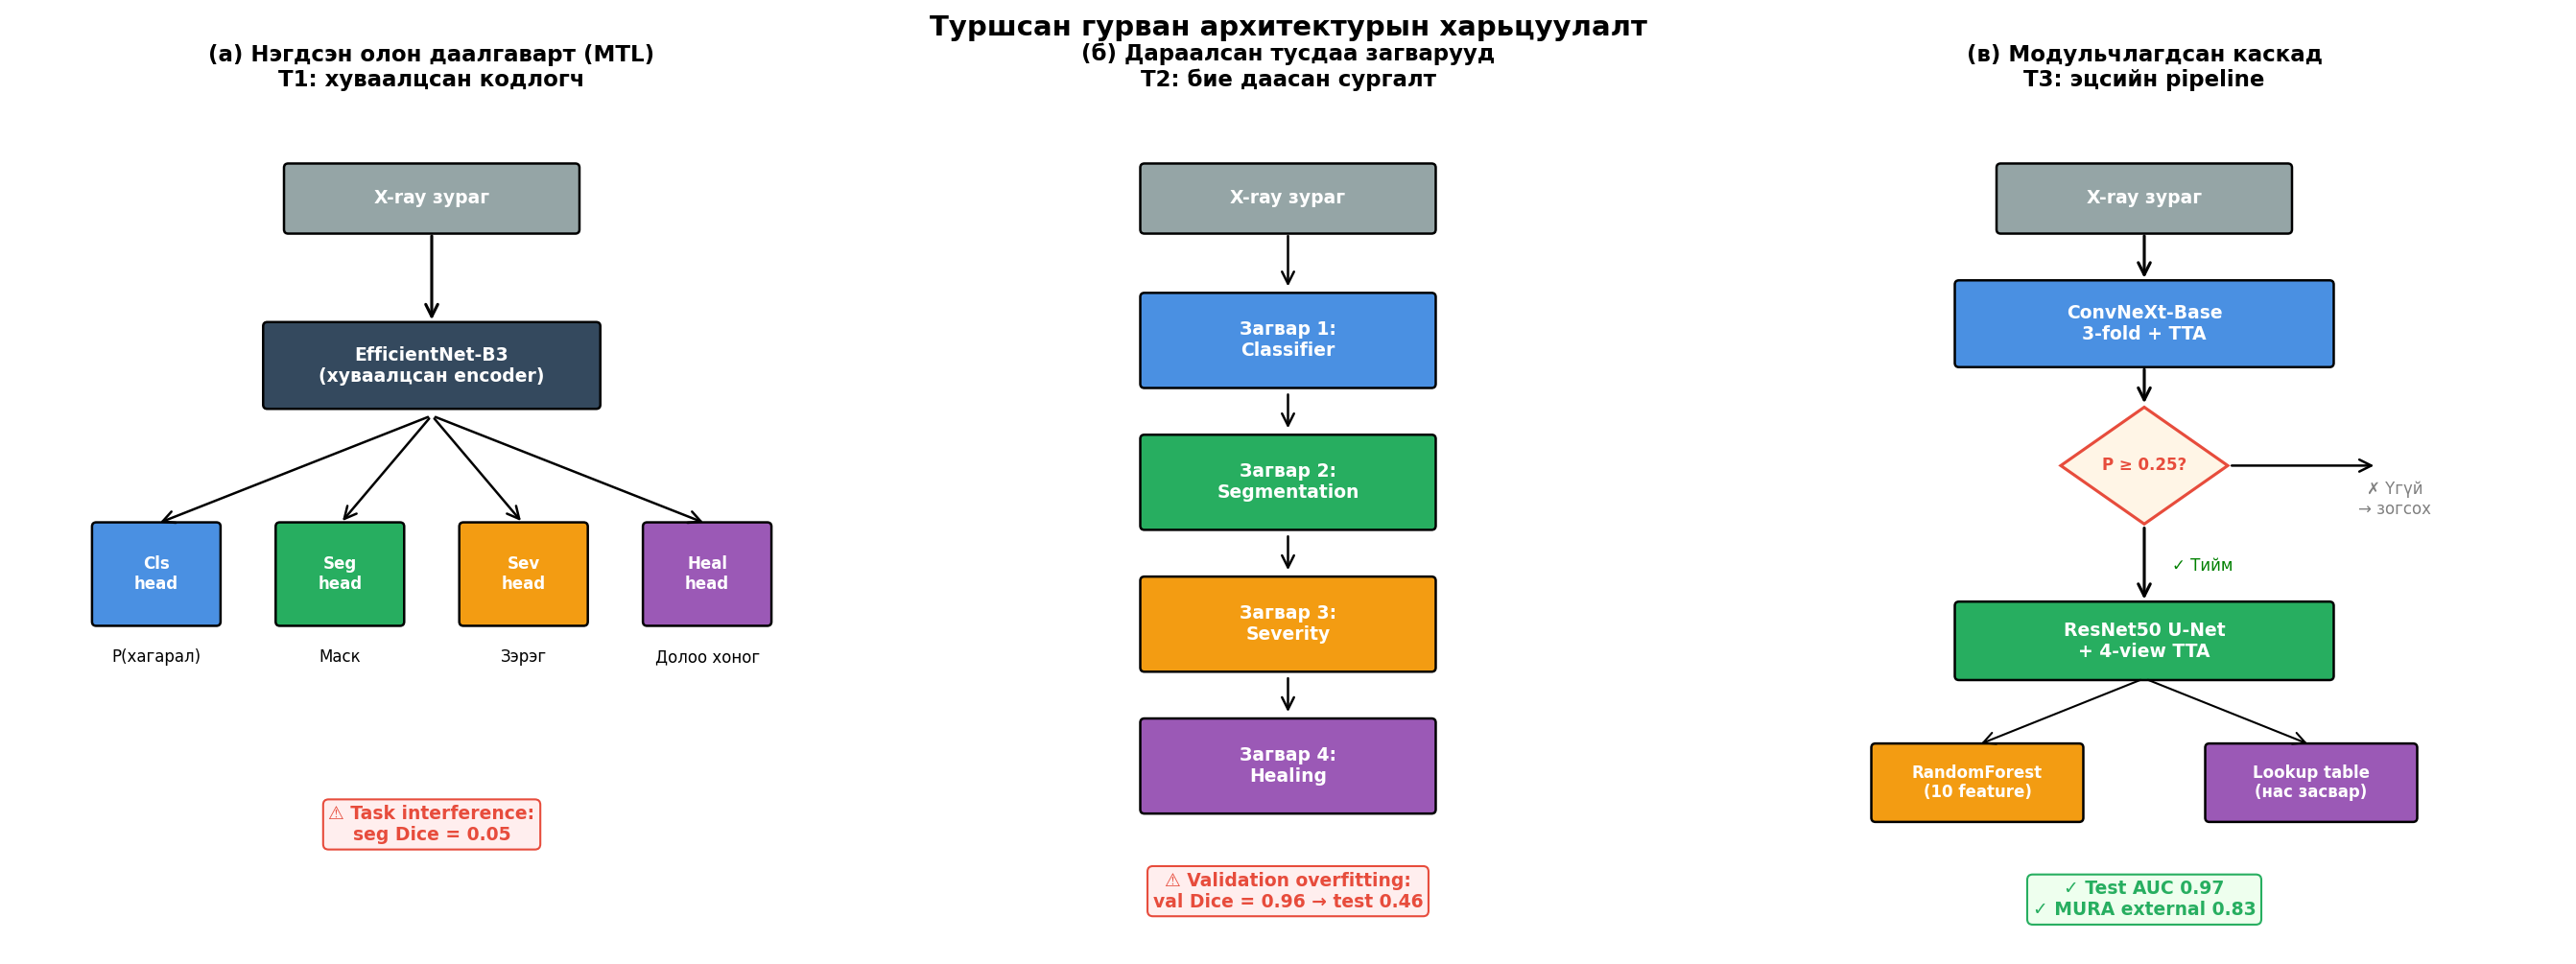
\includegraphics[width=\textwidth]{Figures/Figure_3_1.png}
\figcaption{Туршсан гурван архитектурын харьцуулалт}{Судалгааны явцад туршсан гурван архитектур: (а) нэгдсэн олон даалгаварт (MTL) хуваалцсан кодлогч, (б) дараалсан/тусдаа сургасан загварууд, (в) эцсийн модульчлагдсан каскад pipeline}
\label{fig:three_arch}
\end{figure}

Судалгааны эхний хувилбарт нэг хуваалцсан кодлогч дээр суурилсан олон даалгаварт загвар туршсан. Энэ хувилбарын зорилго нь нэг рентген зургаас нийтлэг дүрслэлийн шинж чанарыг ялган авч, түүнийг ангилал, сегментчлэл, хугарлын зэрэг болон эдгэрэлтийн таамаглалын модулиудад зэрэг ашиглах явдал байв. Харин туршилтын явцад сегментчлэлийн даалгавар бусад даалгавартай хамт сургах үед тогтворгүй болох хандлага илэрсэн тул эцсийн шийдэлд даалгавар тус бүрийг бие даасан модулиар шийдвэрлэх каскад pipeline-ийг сонгосон. Энэ шийдэл нь загвар бүрийг өөрийн өгөгдөл, алдагдлын функц, сургалтын тохиргоонд нь нийцүүлэн оновчлох боломж олгосон.

\subsection{Туршилт 1: хуваалцсан кодлогчтой олон даалгаварт архитектур}

Анхны архитектурын үндсэн кодлогчоор ImageNet дээр урьдчилан сургагдсан EfficientNet-B3 загварыг сонгосон. EfficientNet-B3 нь compound scaling зарчмаар сүлжээний гүн, өргөн болон оролтын нарийвчлалыг тэнцвэртэй өсгөдөг тул харьцангуй цөөн параметртэй боловч дүрсний төлөөлөл гаргах чадвар сайтай архитектур юм~\cite{ref38}. Кодлогчийн сүүлийн feature map-аас Global Average Pooling ашиглан 384 хэмжээст төлөөлөл үүсгэж, үүнийг дараах дөрвөн модулийн оролт болгон ашигласан.

Нэгдүгээрт, ангиллын модуль нь рентген зурагт хугарал байгаа эсэхийг хоёртын ангиллын хэлбэрээр тодорхойлно. Энэ модуль нь кодлогчоос авсан төлөөллийг бүрэн холболтын давхаргуудаар боловсруулж, хугаралтай болон хугаралгүй гэсэн хоёр гаралт үүсгэнэ. Хоёрдугаарт, сегментчлэлийн модуль нь хугарлын хэсгийг пикселийн түвшинд ялгах зорилготой бөгөөд U-Net хэлбэрийн decoder салбарыг ашигласан. Ингэснээр кодлогчийн гаргасан өндөр түвшний шинжүүдийг decoder хэсгээр орон зайн маск болгон сэргээж, ангилал ба сегментчлэлийг нэг архитектурт зэрэг сургах боломж бүрдсэн.

Гуравдугаарт, хугарлын зэргийн модуль нь хугарлын маск болон дүрсний төлөөллийг хамтад нь ашиглан 0--3 зэрэглэлийн үнэлгээ гаргана. FracAtlas өгөгдлийн сангийн хугарлын зэргийн анхны шошго бүрэн биш байсан тул маскийн талбайн харьцаанд үндэслэн прокси зэрэглэл үүсгэж, зэрэглэлийн дараалсан шинжийг хадгалах үүднээс ordinal regression~\cite{ref35} ашигласан. Дөрөвдүгээрт, эдгэрэлтийн таамаглалын модуль нь дүрсний төлөөлөл, хугарлын зэргийн мэдээлэл болон нас, хүйс, анатомийн байршил зэрэг клиникийн мета-өгөгдлийг нэгтгэн эдгэрэлтийн хугацааг долоо хоногоор таамаглах регрессийн даалгавар болгон загварчилсан~\cite{ref43}.

Энэхүү олон даалгаварт хувилбар нь даалгавруудын хооронд мэдлэг хуваалцах боломжтой боловч туршилтын үр дүнгээс харахад сегментчлэлийн даалгаварт сөргөөр нөлөөлөх буюу task interference илэрсэн. Ялангуяа жижиг талбай эзэлдэг хугарлын маск нь ангилал болон регрессийн алдагдлын нөлөөнд дарагдаж, загвар хоосон маск гаргах хандлагатай болсон. Иймээс олон даалгаварт хандлага нь судалгааны чухал эхний алхам болсон боловч эцсийн pipeline-д шууд ашиглахад хангалттай тогтвортой биш гэж үзсэн.

\subsection{Туршилт 2: даалгавар тус бүрийг тусдаа сургах дараалсан архитектур}

Олон даалгаварт хувилбарын task interference-ийг бууруулах зорилгоор хоёр дахь хувилбарт даалгавар бүрийг нэг архитектурт нэгтгэхгүйгээр, тусдаа загваруудаар дараалан сургах аргыг туршсан. Энэ хувилбарт ангиллын загварыг MURA өгөгдөл дээр, сегментчлэл болон хугарлын зэргийн загварыг FracAtlas дээр, эдгэрэлтийн загварыг GRAZPEDWRI-DX-ийн мета-өгөгдөлд тулгуурлан тус тусад нь сургав. Модуль бүр өөрийн алдагдлын функц, оролтын хэмжээ болон сургалтын тохиргоотой байсан тул нэгдсэн загвартай харьцуулахад сегментчлэлийн сургалт мэдэгдэхүйц тогтворжсон.

Гэвч энэхүү хувилбарт сегментчлэлийн загвар баталгаажуулалтын олонлог дээр маш өндөр Dice (\(\approx 0.96\)) үзүүлсэн ч энэ нь баталгаажуулалтын өгөгдөлд хэт тохирох (overfitting) шинжтэй байсан тул бие даасан тест олонлог дээр ерөнхийлөх чадвар нь хангалтгүй байв. Иймээс дараалсан сургалт нь зөв чиглэлийн алхам боловч сегментчлэлийн жинхэнэ тогтворжилт болон ерөнхийлөх чадварыг бүрэн хангаагүй гэж дүгнэв. Энэ ажиглалт нь сургалтын стратеги (хоёр үе шаттай урьдчилсан сургалт, чанарын шүүлтүүр, TTA) болон илүү хүчтэй кодлогч шаардлагатайг харуулсан бөгөөд эцсийн модульчлагдсан хувилбарыг боловсруулах үндэслэл болсон.

\subsection{Туршилт 3: ConvNeXt ба ResNet50 U-Net-д суурилсан модульчлагдсан архитектур}

Эцсийн архитектур нь даалгавар тус бүрийг тусдаа загвараар шийдвэрлэх каскад бүтэцтэй. Энэ бүтэц нь эмнэлзүйн ажлын дараалалтай нийцнэ: эхлээд хугарал байгаа эсэхийг шалгаж, хугарал илэрсэн тохиолдолд байршлыг нь тодорхойлж, дараа нь хугарлын зэргийг үнэлэн эдгэрэлтийн хугацааг тооцно. Ийнхүү ангиллын модуль нь pipeline-ийн эхний шүүлтүүрийн үүрэгтэй, сегментчлэлийн модуль нь тайлбарлагдах байршлын мэдээлэл өгдөг, хугарлын зэргийн модуль нь маскаас гарсан морфологийн шинжүүдийг ашигладаг, эдгэрэлтийн модуль нь дүрс болон клиникийн мэдээллийг нэгтгэн регрессийн таамаглал гаргадаг.

Ангиллын модульд ImageNet-22K дээр урьдчилан сургагдсан ConvNeXt архитектурыг ашигласан. ConvNeXt нь CNN-ийн орон зайн inductive bias-ийг хадгалсан боловч орчин үеийн vision transformer загваруудын сургалтын зарим зарчмыг тусгасан тул эмнэлгийн дүрсний нарийн ялгааг танихад тохиромжтой гэж үзсэн. Ангиллын толгой нь бинар сигмоид гаралттай бөгөөд ангийн тэнцвэргүй байдлыг бууруулахын тулд Focal BCE алдагдал~\cite{ref44}, жинлэсэн sampling болон өгөгдөл нэмэгдүүлэх аргуудыг хэрэглэсэн.

ConvNeXt-ийг сонгосон үндсэн шалтгаан нь рентген зураг дээрх хугарлын шинж нь ихэвчлэн жижиг, локал, контраст багатай бүтэц хэлбэрээр илэрдэгтэй холбоотой. Уламжлалт CNN загварууд ийм орон зайн шинжийг сайн хадгалдаг боловч гүнзгий шатанд мэдээлэл бүдгэрэх, жижиг ан цавын ялгаа дарагдах эрсдэлтэй. ConvNeXt-ийн том kernel бүхий depthwise convolution, шаталсан feature hierarchy, LayerNorm болон GELU-д суурилсан блокийн бүтэц нь ийм нарийн дүрслэлийн ялгааг илүү тогтвортой ялгах боломжтой гэж үзсэн.

Мөн ImageNet-22K дээр урьдчилан сургасан ConvNeXt-Base хувилбар нь ImageNet-1K дээр сургасан жижиг загваруудаас илүү өргөн дүрслэлийн төлөөлөл сурсан байдаг. Эмнэлгийн рентген зураг нь судалгааны өгөгдлийн хэмжээгээр хязгаарлагдмал тул том хэмжээний ерөнхий дүрсний өгөгдөл дээр сурсан backbone ашиглах нь overfitting-ийг бууруулах, олон эх сурвалжийн зураг дээр ерөнхийлөх чадварыг нэмэгдүүлэх давуу талтай. Туршилтын харьцуулалтаар ConvNeXt-Base нь ResNet-50, EfficientNet-B3 болон ConvNeXt-Small загваруудаас өндөр AUC, F1 үзүүлсэн тул эцсийн ангиллын модуль болгон сонгосон.

Сегментчлэлийн модульд ResNet50~\cite{he2016resnet} кодлогчтой U-Net~\cite{ronneberger2015unet} архитектурыг ашигласан. Анхны $224\times224$ хэмжээ нь нарийн хугарлын шугамыг хангалттай хадгалж чадахгүй байсан тул сегментчлэлийн оролтыг $512\times512$ болгож нэмэгдүүлсэн. U-Net-ийн skip connection бүтэц нь доод түвшний ирмэг, хэлбэрийн мэдээллийг decoder хэсэгт шууд дамжуулдаг тул жижиг, нарийн хугарлын бүсийг сэргээхэд илүү тохиромжтой. Сургалтад FracAtlas-ийн гараар тэмдэглэсэн маскуудаас гадна SAM-аар үүсгэсэн псевдо маскуудыг чанарын шүүлтүүрээр дамжуулан ашигласан.

Хугарлын зэргийн үнэлгээнд зөвхөн хар хайрцаг хэлбэрийн ангилагч ашиглахын оронд сегментчлэлийн маскаас талбай, хэлбэр, чиглэл, хэсгийн тоо зэрэг морфологийн шинжүүдийг тооцох хандлага сонгосон. Энэ нь хугарлын зэрэглэлийг тайлбарлах боломжийг нэмэгдүүлж, эмч тухайн үнэлгээ ямар дүрсний шинжид үндэслэснийг шалгах нөхцөл бүрдүүлнэ. Гэхдээ хугарлын зэргийн шошго нь эмчийн бүрэн клиникийн үнэлгээ биш, морфологийн шинжид суурилсан прокси үнэлгээ тул энэ модулийг клиникийн баталгаажсан зэрэглэл тогтоогч бус, proof-of-concept түвшний модуль гэж авч үзсэн.

Эдгэрэлтийн модуль нь хугарлын зэрэг, анатомийн байршил, нас, хүйс зэрэг шинжүүдийг ашиглан эдгэрэлтийн хугацааг долоо хоногоор таамаглах регрессийн загвар хэлбэрээр боловсруулагдсан. Гэхдээ энэ хэсэгт бодит урт хугацааны клиникийн follow-up өгөгдөл дутагдалтай тул синтетик өгөгдөл ашигласан нь судалгааны нэг үндсэн хязгаарлалт болно. Иймээс эдгэрэлтийн модулийн үр дүнг мөн proof-of-concept буюу цаашид бодит клиникийн өгөгдлөөр баталгаажуулах шаардлагатай боломжийн баталгаа гэж тайлбарлав.

\subsection{Эцсийн pipeline-ийн оролт, завсрын гаралт ба шийдвэрийн урсгал}

Санал болгож буй pipeline-ийн ажиллагааг дараах дарааллаар нэгтгэн тодорхойлж болно.

\begin{enumerate}[nosep]
    \item Оролтын рентген зургийг стандарт хэмжээнд хөрвүүлж, нормчлол болон шаардлагатай нэмэлт боловсруулалтыг гүйцэтгэнэ.
    \item Ангиллын загвар зурагт хугарал байх магадлалыг тооцно. Хэрэв магадлал тогтоосон босгоос бага бол зураг хугаралгүй гэж тэмдэглэгдэж, дараагийн модулиуд ажиллахгүй.
    \item Хугарал илэрсэн зурагт сегментчлэлийн загвар ажиллаж, хугарлын бүсийн хоёртын маскийг үүсгэнэ.
    \item Маскаас морфологийн шинжүүдийг тооцож, хугарлын зэргийг 0--3 шатлалаар үнэлнэ.
    \item Дүрсний болон клиникийн шинжүүдийг нэгтгэн эдгэрэлтийн хугацааны таамаглалыг гаргана.
\end{enumerate}

Энэхүү бүтэц нь нэг загвараар бүх даалгаврыг зэрэг шийдвэрлэхээс илүү уян хатан бөгөөд аль нэг модульд сайжруулалт хийхэд бусад хэсгийг бүхэлд нь дахин сургах шаардлагыг бууруулна. Мөн ангиллын итгэлийн оноо, сегментчлэлийн маск, морфологийн шинжүүд зэрэг завсрын гаралтууд нь загварын шийдвэрийг тайлбарлах боломжийг нэмэгдүүлдэг. Иймээс санал болгож буй архитектурыг бие даасан оношилгооны систем бус, харин эмчийн шийдвэрийг дэмжих судалгааны түвшний pipeline гэж үзнэ.

%-------------------------------------------------------------------------------

\section{Өгөгдөл цуглуулах арга}

Судалгаанд ашиглах өгөгдлийг сонгохдоо хоёр үндсэн шалгуурыг баримталсан. Нэгдүгээрт, өгөгдлийн сан нь рентген зурагт суурилсан ясны хугарлын судалгаанд ашиглах боломжтой, нийтэд нээлттэй, судалгааны зориулалтаар ашиглах нөхцөл нь тодорхой байх шаардлагатай. Хоёрдугаарт, өгөгдөл нь энэхүү ажлын дөрвөн үндсэн даалгаврын аль нэгийг дэмжихүйц шошго, тэмдэглэгээ эсвэл мета-өгөгдөл агуулсан байх ёстой. Иймээс нэг өгөгдлийн сангаар бүх даалгаврыг шийдвэрлэх боломжгүй тул хэд хэдэн эх сурвалжийг зорилтот даалгаварт нь тохируулан нэгтгэн ашиглав.

Ангиллын даалгаврын өгөгдлийг туршилтын үе шат бүрийн зорилгод нийцүүлэн сонгосон. Эхний хоёр туршилтад MURA өгөгдлийн санг хэвийн болон гажигтай рентген зургийг ялгах суурь сургалтад ашигласан~\cite{ref39}. Харин эцсийн буюу гурав дахь туршилтын ангиллын модульд GRAZPEDWRI-DX, FracAtlas-COCO, YOLOBoneFracture болон BoneFractureCVProject өгөгдлийн сангуудыг нэгтгэн ашигласан~\cite{ref40,ref41}. Эдгээр эх сурвалжийг нэгтгэснээр хугаралтай болон хугаралгүй жишээний төрөлжилтийг нэмэгдүүлж, ангиллын загвар нэг өгөгдлийн сангийн дүрсний хэв шинжид хэт тохирох эрсдэлийг бууруулахыг зорьсон.

Сегментчлэлийн даалгаварт FracAtlas-ийн масктай зургуудыг үндсэн эх сурвалж болгон авсан. Гэвч гараар тэмдэглэсэн масктай зураг цөөн тул YOLOBoneFracture болон BoneFractureCVProject өгөгдлийн сангийн хайрцаг тэмдэглэгээг ашиглан SAM-д суурилсан псевдо маск үүсгэж, сегментчлэлийн сургалтын өгөгдлийг өргөтгөсөн. Энэ шийдэл нь хугарлын бүсийг пикселийн түвшинд суралцахад шаардлагатай жишээний тоог нэмэгдүүлэх зорилготой бөгөөд псевдо шошгоны чанарыг тусгай шүүлтүүрээр шалгасан.

Хугарлын зэргийн үнэлгээнд FracAtlas-ийн сегментчлэлийн маск болон түүнээс тооцоолсон морфологийн шинжүүдийг ашигласан. Анхны өгөгдлийн сан дахь хугарлын зэргийн шошго бүрэн биш тул хугарлын маскийн талбай, хэлбэр, чиглэл зэрэг дүрсний шинжид тулгуурлан зэрэглэлийн прокси мэдээлэл үүсгэсэн. Энэ нь эмчийн клиникийн үнэлгээг бүрэн орлохгүй боловч хугарлын дүрслэлийн хэмжигдэхүйц шинжүүд хугарлын зэрэгтэй хэрхэн уялдахыг турших боломж олгосон.

Эдгэрэлтийн таамаглалын хувьд ашигласан нээлттэй рентген зургийн сангуудад бодит эдгэрэлтийн хугацааны урт хугацааны шошго байхгүй байсан. Иймээс GRAZPEDWRI-DX-ийн нас, хүйс зэрэг мета-өгөгдлийг ашиглахын зэрэгцээ эмнэлзүйн лавлагаанд суурилсан синтетик клиникийн өгөгдөл үүсгэн туршилтын түвшинд хэрэглэв. Синтетик өгөгдөл нь бодит өвчтөний мэдээлэл агуулаагүй тул нууцлалын эрсдэл багатай боловч клиникийн бодит өгөгдлийг бүрэн төлөөлөхгүй. Иймээс эдгэрэлтийн модулийн үр дүнг судалгааны туршилтын хүрээнд тайлбарлав.

Өгөгдлийн сан бүрийн лиценз, ёс зүйн нөхцөл, урьдчилсан боловсруулалт, хуваалт болон чанарын шалгалтыг \ref{Chapter4}~бүлэгт дэлгэрэнгүй авч үзсэн. Энэ хэсэгт зөвхөн өгөгдлийн эх сурвалжуудыг ямар үндэслэлээр сонгож, судалгааны даалгавруудад хэрхэн хуваарилсныг нэгтгэн тодорхойлов.

%-------------------------------------------------------------------------------

\section{AI хэрэгслийн ашиглалт ба ил тод байдал}

Судалгааны ажлын явцад хиймэл оюунд суурилсан туслах хэрэгслийг зөвхөн хязгаарлагдмал, туслах зориулалтаар — бичвэрийн найруулга, үг үсэг, хэл зүйн алдаа шалгах, \LaTeX{} форматлалыг тодруулах болон кодын алдаа засахад зөвлөмж авахад ашигласан. Харин судалгааны сэдэв, арга зүй, өгөгдлийн сонголт, загварын архитектур, туршилтын төлөвлөлт, кодын хэрэгжүүлэлт болон үр дүнгийн шинжилгээг судлаач өөрөө боловсруулж гүйцэтгэсэн бөгөөд хиймэл оюуны хэрэгсэл нь өгөгдөл үүсгэх, туршилт хийх, үр дүн тооцоолох болон дүгнэлт гаргах үүрэг гүйцэтгээгүй болно.

%\pagecolor{Beige}
% !TEX root = ../main.tex
% Бүлэг 4

\chapter{Өгөгдөл боловсруулалт}
\label{Chapter4}
\pagecolor{Beige}

%-------------------------------------------------------------------------------

\section{Өгөгдлийн эх сурвалж ба зөвшөөрөл}

Судалгаанд нийтэд нээлттэй зургаан рентген зургийн өгөгдлийн сан болон эдгэрэлтийн таамаглалд зориулсан нэг синтетик клиникийн өгөгдлийг ашигласан. Эдгээр эх сурвалжуудыг сонгохдоо судалгааны зориулалтаар ашиглах боломж, лицензийн тодорхой байдал, өвчтөний мэдээлэл нэргүйжүүлэгдсэн эсэх, мөн тухайн өгөгдөл нь ангилал, сегментчлэл, хугарлын зэрэг болон эдгэрэлтийн таамаглалын аль даалгаварт тохирохыг харгалзав.

MURA өгөгдлийн сан нь яс-булчингийн рентген зургаар баялаг бөгөөд эхний хоёр туршилтад хэвийн болон гажигтай дүрсийг ялгах ангиллын суурь өгөгдөл болсон~\cite{ref39}. Харин эцсийн модульчлагдсан pipeline-д MURA-г шууд сургалтын өгөгдөл болгон ашиглаагүй. FracAtlas нь хугарлын тодорхой жишээ, COCO форматтай маск болон хугарлын мета-өгөгдөл агуулдаг тул сегментчлэл болон хугарлын зэргийн үнэлгээнд гол эх сурвалж болж ашиглагдсан~\cite{ref40}. GRAZPEDWRI-DX нь хүүхдийн бугуйн рентген зураг, YOLO тэмдэглэгээ болон нас, хүйсийн мэдээлэл агуулдаг тул Туршилт 3-ын ангиллын өгөгдлийн үндсэн эх сурвалжуудын нэг болсон~\cite{ref41}.

Туршилт 3-ын ангиллын модульд GRAZPEDWRI-DX, FracAtlas-COCO, YOLOBoneFracture болон BoneFractureCVProject өгөгдлийн сангуудыг ашигласан. YOLO хайрцаг тэмдэглэгээтэй өгөгдлүүдийг Туршилт 3-ыг эхлүүлэхээс өмнөх өгөгдөл бэлтгэлийн шатанд SAM загварт prompt болгон дамжуулж, сегментчлэлийн псевдо масктай жишээ үүсгэхэд хэрэглэсэн. Эдгэрэлтийн бодит хугацааны урт хугацааны тэмдэглэгээ нээлттэй өгөгдлийн сангуудад байхгүй байсан тул синтетик клиникийн өгөгдлийг зөвхөн proof-of-concept түвшинд ашигласан.

\begin{table}[H]
    \centering
    \caption{Судалгаанд ашигласан өгөгдлийн эх сурвалжууд}
    \label{tab:dataset_sources}
    \scriptsize
    \begin{tabularx}{\textwidth}{@{}>{\raggedright\arraybackslash}p{2.15cm}
        >{\raggedright\arraybackslash}p{1.55cm}
        >{\raggedright\arraybackslash}p{2.35cm}
        >{\raggedright\arraybackslash}X
        >{\raggedright\arraybackslash}p{1.65cm}@{}}
    \toprule
    \textbf{Өгөгдөл} & \textbf{Хэмжээ} & \textbf{Тэмдэглэгээ} & \textbf{Ашигласан зорилго} & \textbf{Лиценз} \\
    \midrule
    MURA & $\sim$40,000 зураг & Normal/ abnormal & Туршилт 1--2-ын ангиллын суурь өгөгдөл & Судалгааны зориулалт \\
    FracAtlas & 4,083 зураг & Binary, COCO mask & Сегментчлэл, хугарлын зэрэг & CC BY 4.0 \\
    \shortstack[l]{GRAZPEDWRI\\-DX} & 20,327 зураг & YOLO bbox, нас/хүйс & Туршилт 3-ын ангилал & CC BY 4.0 \\
    \shortstack[l]{FracAtlas\\-COCO} & 966 зураг & COCO JSON & Туршилт 3-ын ангилал & CC BY 4.0 \\
    \shortstack[l]{YOLOBone\\Fracture} & 3,979 зураг & YOLO bbox & Туршилт 3-ын ангилал, псевдо маск бэлтгэл & CC0 \\
    \shortstack[l]{BoneFracture\\CVProject} & 3,631 зураг & YOLO bbox & Туршилт 3-ын ангилал, псевдо маск бэлтгэл & CC BY 4.0 \\
    Синтетик өгөгдөл & 5,000 мөр & Клиникийн хувьсагч & Эдгэрэлтийн таамаглал & Зохиомол \\
    \bottomrule
    \end{tabularx}
\end{table}

Бүх рентген зургийн өгөгдөл нь нийтэд нээлттэй хэлбэрээр түгээгдсэн бөгөөд өвчтөний шууд таних мэдээлэл агуулаагүй. Гэсэн хэдий ч өгөгдөл бүрийн лиценз, эх сурвалжийн нөхцөлийг хүндэтгэн зөвхөн судалгааны болон туршилтын зорилгоор ашиглав. Синтетик өгөгдөл нь бодит өвчтөний мэдээлэл агуулаагүй тул хувийн нууцын шууд эрсдэл бага боловч бодит клиникийн өгөгдлийг бүрэн төлөөлөхгүй гэсэн хязгаарлалтыг үр дүнгийн тайлбарт харгалзан үзсэн.

%-------------------------------------------------------------------------------

\section{Урьдчилсан боловсруулалт ба өгөгдөл нэмэгдүүлэлт}

Өгөгдлийн сангууд нь өөр өөр эх сурвалжаас бүрдсэн тул дүрсний хэмжээ, формат, суваг, тодрол, тэмдэглэгээний хэлбэр харилцан адилгүй байв. Иймээс сургалтад оруулахын өмнө дүрс бүрийг нэгэн ижил pipeline-аар боловсруулж, загварын оролтын шаардлагад нийцүүлсэн.

\subsection*{Дүрсний урьдчилсан боловсруулалт}

Эхний шатанд бүх зургийг уншиж, эвдэрсэн эсвэл дутуу файлыг хассан. Grayscale хэлбэртэй зургуудыг гурван сувагтай болгож, ImageNet дээр урьдчилан сургагдсан загваруудын оролтын хэлбэртэй нийцүүлэв. Ангиллын даалгаварт оролтын хэмжээг ихэвчлэн $224\times224$ болгосон бол сегментчлэлийн даалгаварт хугарлын нарийн шугамыг хадгалахын тулд $512\times512$ хэмжээг ашигласан.

Пикселийн утгыг $[0,255]$ завсраас $[0,1]$ завсарт хөрвүүлж, дараа нь ImageNet-ийн дундаж болон стандарт хазайлтаар нормчилсон. Энэ нь урьдчилан сургагдсан ConvNeXt, EfficientNet болон ResNet төрлийн загваруудыг ашиглах үед оролтын тархалтыг сургалтын эх тархалттай ойролцоо байлгах зорилготой.

\begin{equation}
    \hat{x} = \frac{x/255 - \mu_{\text{IN}}}{\sigma_{\text{IN}}}, \quad
    \mu_{\text{IN}} = [0.485,\ 0.456,\ 0.406], \quad
    \sigma_{\text{IN}} = [0.229,\ 0.224,\ 0.225]
\end{equation}

Дүрсний урьдчилсан боловсруулалтын үндсэн алхмуудыг (анхны зураг, хэмжээ өөрчлөлт, нормчлол) Зураг~\ref{fig:preprocess_steps}-д үзүүлэв.

\begin{figure}[H]
    \centering
    \begin{minipage}{0.31\textwidth}\centering
        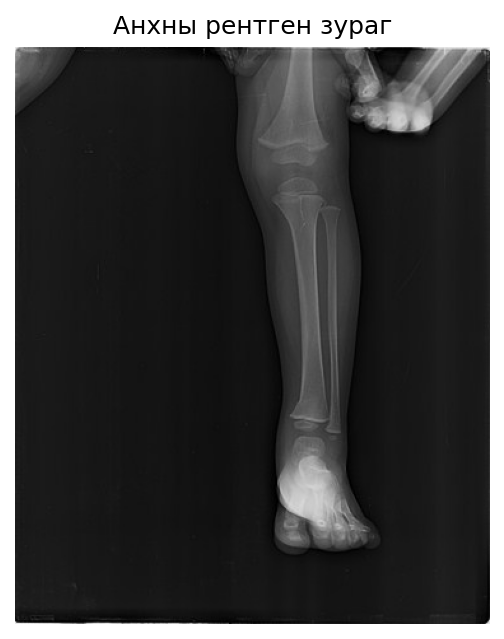
\includegraphics[width=\linewidth,height=0.26\textheight,keepaspectratio]{Figures/appx_b1_original.png}\\{\scriptsize (а) Анхны зураг}
    \end{minipage}\hfill
    \begin{minipage}{0.31\textwidth}\centering
        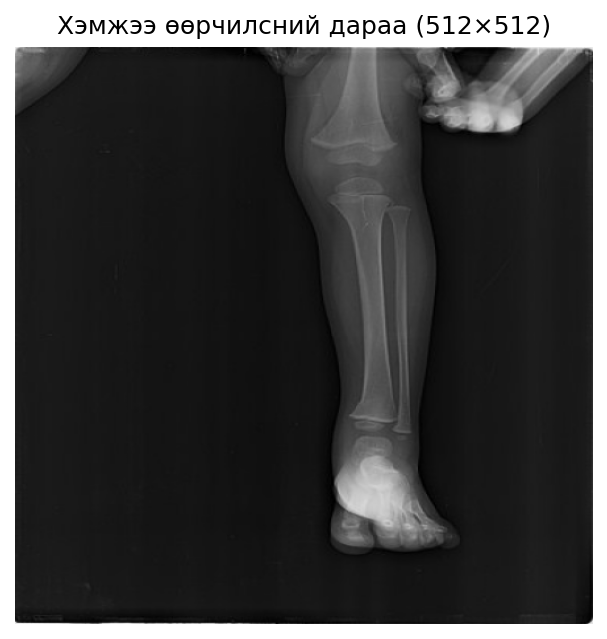
\includegraphics[width=\linewidth,height=0.26\textheight,keepaspectratio]{Figures/appx_b2_resized.png}\\{\scriptsize (б) Хэмжээ өөрчилсөн}
    \end{minipage}\hfill
    \begin{minipage}{0.31\textwidth}\centering
        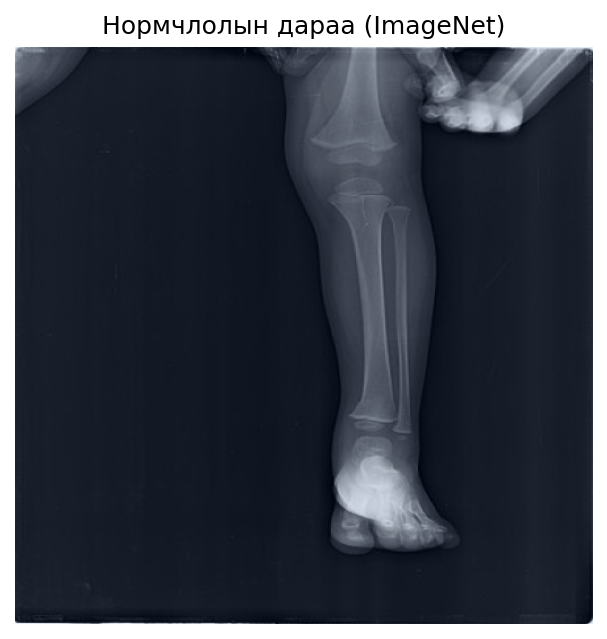
\includegraphics[width=\linewidth,height=0.26\textheight,keepaspectratio]{Figures/appx_b3_normalized.png}\\{\scriptsize (в) Нормчилсон}
    \end{minipage}
    \figcaption{Дүрсийн урьдчилсан боловсруулалтын алхмууд}{Дүрсийн урьдчилсан боловсруулалтын алхмууд: (а) анхны рентген зураг, (б) хэмжээ өөрчилсний дараах, (в) нормчлол хийсний дараах}
    \label{fig:preprocess_steps}
\end{figure}

FracAtlas-ийн COCO polygon тэмдэглэгээг хоёртын маск болгон хувиргасан. Маскийг resize хийхдээ nearest-neighbor interpolation хэрэглэсэн бөгөөд энэ нь маскийн 0 ба 1 утгын хоёртын шинжийг хадгалах давуу талтай. Харин рентген зургийн хэмжээг өөрчлөхөд bilinear interpolation ашигласан.

Туршилт 3-ыг эхлүүлэхээс өмнө YOLOBoneFracture болон BoneFractureCVProject өгөгдлийн сангийн YOLO хайрцаг тэмдэглэгээг SAM загварт prompt болгон өгч, хугарлын бүсийн псевдо маск үүсгэсэн. Энэ алхам нь эхний хоёр туршилтын сургалтад ашиглагдаагүй бөгөөд зөвхөн Туршилт 3-ын сегментчлэлийн өгөгдлийг өргөтгөх бэлтгэл ажил байсан. Үүссэн псевдо маскуудыг итгэлийн оноо, маскийн талбай, хоосон маск болон металл implant-ийн нөлөө зэрэг шалгуураар шүүж, чанарын шаардлага хангаагүй жишээг сургалтад оруулаагүй.

\subsection*{Мета-өгөгдөл ба шошго нэгтгэл}

Ангиллын даалгаварт эх сурвалж бүрийн шошгыг хугаралтай болон хугаралгүй гэсэн хоёртын хэлбэрт нэгтгэсэн. MURA-ийн abnormal шошго нь заавал хугарал гэсэн утгатай биш тул уг өгөгдлийг зөвхөн эхний хоёр туршилтад ерөнхий эмгэг өөрчлөлт ялгах суурь мэдлэг олгох зорилгоор ашигласан. Эцсийн ConvNeXt-Base ангилагчид GRAZPEDWRI-DX, FracAtlas-COCO, YOLOBoneFracture болон BoneFractureCVProject өгөгдлийг ашигласан бөгөөд эдгээр нь Туршилт 3-ын ангиллын сургалтын үндсэн эх сурвалж болсон.

Хугарлын зэргийн хувьд эх өгөгдөлд эмчийн бүрэн 0--3 шатлалтай шошго байхгүй тул FracAtlas-ийн маск болон түүнээс гарсан морфологийн шинжүүдийг ашигласан. Маскийн талбай, хэлбэр, чиглэл, хэсгийн тоо зэрэг шинжүүдээр хугарлын зэргийн прокси мэдээлэл үүсгэсэн бөгөөд энэ нь клиникийн эцсийн үнэлгээг орлохгүй, зөвхөн дүрслэлийн хэмжигдэхүйц шинжид суурилсан proof-of-concept үнэлгээ юм.

GRAZPEDWRI-DX-ийн файлын нэр болон мета-өгөгдлөөс нас, хүйс зэрэг хувьсагчдыг ялган авч, эдгэрэлтийн таамаглалын оролтын нэг хэсэг болгон ашигласан. Эдгэрэлтийн хугацааны бодит шошго байхгүй тул эдгээр хувьсагчийг синтетик клиникийн өгөгдөлтэй хослуулан proof-of-concept түвшинд хэрэглэв.

\subsection*{Өгөгдөл нэмэгдүүлэлт}

Өгөгдөл нэмэгдүүлэлтийг зөвхөн сургалтын хуваалтад хэрэглэсэн. Баталгаажуулалт болон тестийн хуваалтад өгөгдөл нэмэгдүүлэх арга хэрэглэхгүй байж, загварын бодит ерөнхийлөх чадварыг хэмжих зарчим баримталсан. Нэмэлт хувиргалтуудыг сонгохдоо рентген зураг авах үеийн байрлал, тодрол, шуугиан болон аппаратын ялгааг дуурайх боломжтой эсэхийг харгалзсан.

\begin{table}[H]
    \centering
    \caption{Урьдчилсан боловсруулалт ба өгөгдөл нэмэгдүүлэлтийн нэгтгэл}
    \label{tab:preprocess_augmentation}
    \small
    \begin{tabular}{p{3.6cm} p{4.4cm} p{4.4cm}}
    \toprule
    \textbf{Алхам} & \textbf{Арга} & \textbf{Зорилго} \\
    \midrule
    Хэмжээ нэгтгэх & $224\times224$ ангилал, $512\times512$ сегментчлэл & Загварын оролтыг стандартчилах \\
    Суваг нэгтгэх & Grayscale зургийг 3 сувагт хөрвүүлэх & Урьдчилан сургагдсан загварт нийцүүлэх \\
    Нормчлол & ImageNet mean/std & Оролтын тархалтыг тогтворжуулах \\
    Маск хөрвүүлэх & COCO polygon $\rightarrow$ binary mask & Сегментчлэлийн ground truth бэлтгэх \\
    CLAHE & Орон нутгийн контраст нэмэгдүүлэх & Хугарлын нарийн шугамыг тодруулах \\
    Геометрийн хувиргалт & Эргүүлэлт, тусгал, тайралт & Байрлалын хэлбэлзэлд тэсвэртэй болгох \\
    Пикселийн хувиргалт & Тодрол, контраст, Gaussian noise & Дүрсний чанарын хэлбэлзлийг дуурайх \\
    Mixup~\cite{zhang2018mixup} & $\alpha=0.2$ & Ангиллын ерөнхийлөх чадварыг нэмэгдүүлэх \\
    \bottomrule
    \end{tabular}
\end{table}

Сегментчлэлийн даалгаварт зураг болон масктай холбоотой геометрийн хувиргалтыг ижил параметрээр хэрэглэсэн. Харин тодрол, контраст, шуугиан зэрэг пикселийн түвшний хувиргалтыг зөвхөн зурагт хэрэглэж, маскийг өөрчлөөгүй. Энэ нь хугарлын байрлалын шошгыг зөрүүлэхгүй байх шаардлагатай холбоотой. Сургалтын хуваалтад хэрэглэсэн өгөгдөл нэмэгдүүлэлтийн жишээг Зураг~\ref{fig:augment_example}-д үзүүлэв.

\begin{figure}[H]
    \centering
    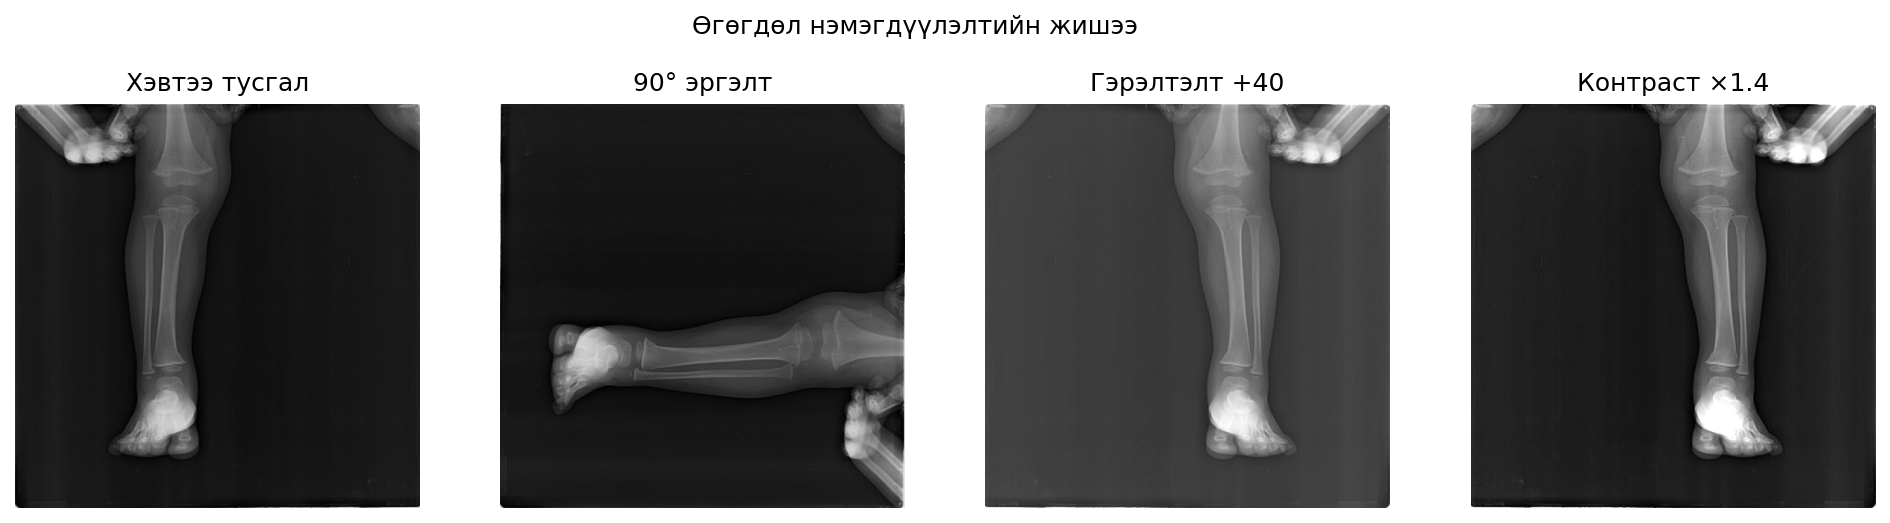
\includegraphics[width=0.85\textwidth,height=0.34\textheight,keepaspectratio]{Figures/appx_b4_augment.png}
    \figcaption{Өгөгдөл нэмэгдүүлэлтийн жишээ}{Сургалтын хуваалтад хэрэглэсэн өгөгдөл нэмэгдүүлэлтийн жишээ}
    \label{fig:augment_example}
\end{figure}

%-------------------------------------------------------------------------------

\section{Train/validation/test хуваалт}

Загварын гүйцэтгэлийг бодитой үнэлэхийн тулд өгөгдлийг сургалт, баталгаажуулалт, тестийн гурван хэсэгт хуваасан. Сургалтын хэсгийг загварын параметр сурахад, баталгаажуулалтын хэсгийг гиперпараметр болон босго утга сонгоход, тестийн хэсгийг зөвхөн эцсийн гүйцэтгэлийг хэмжихэд ашигласан. Ингэснээр тестийн мэдээлэл сургалтын явцад урьдчилан нөлөөлөхөөс сэргийлсэн. Хүснэгт~\ref{tab:data_split}-д өгөгдлийн сан бүрт баримталсан ойролцоох хуваалтын зарчмыг нэгтгэн үзүүлэв.

Хуваалт хийхдээ боломжтой тохиолдолд ангийн харьцааг хадгалах stratified split ашигласан. Нэг өвчтөн эсвэл нэг судалгаанд хамаарах олон зураг байвал нэг хуваалтад хамтад нь байлгах зарчим баримталсан. Энэ нь ижил өвчтөний ойролцоо зураг train болон test-д зэрэг орох data leakage-ийн эрсдэлийг бууруулна. Дахин давтагдах чадварыг хангахын тулд санамсаргүй хуваалт хийх үед тогтмол seed ашигласан.

\begin{table}[H]
    \centering
    \caption{Өгөгдлийн хуваалтын ерөнхий зарчим}
    \label{tab:data_split}
    \small
    \begin{tabular}{p{3.1cm} p{2.2cm} p{2.2cm} p{2.2cm} p{3.3cm}}
    \toprule
    \textbf{Өгөгдөл} & \textbf{Train} & \textbf{Validation} & \textbf{Test} & \textbf{Тэмдэглэл} \\
    \midrule
    MURA & 70--80\% & 10--15\% & 10--15\% & Туршилт 1--2-ын ангиллын суурь сургалт \\
    FracAtlas & 70--80\% & 10--15\% & 10--15\% & Масктай хэсгийг сегментчлэлд ашигласан \\
    \shortstack[l]{GRAZPEDWRI\\-DX} & 70--80\% & 10--15\% & 10--15\% & Нас, хүйсийн хувьсагч ялгасан \\
    \shortstack[l]{FracAtlas\\-COCO} & 70\% & 15\% & 15\% & Туршилт 3-ын ангилал \\
    \shortstack[l]{YOLOBone\\Fracture} & 70\% & 15\% & 15\% & Туршилт 3-ын ангилал, псевдо маск бэлтгэл \\
    \shortstack[l]{BoneFracture\\CVProject} & 70\% & 15\% & 15\% & Туршилт 3-ын ангилал, псевдо маск бэлтгэл \\
    Синтетик өгөгдөл & 80\% & 10\% & 10\% & Эдгэрэлтийн туршилтын модуль \\
    \bottomrule
    \end{tabular}
\end{table}

Эхний хоёр туршилтад MURA өгөгдлийг ангиллын суурь сургалтад ашигласан. Харин эцсийн ConvNeXt-Base ангилагчийн сургалтад GRAZPEDWRI-DX, FracAtlas-COCO, YOLOBoneFracture болон BoneFractureCVProject өгөгдлийг нэгтгэн нийт 28,903 зураг ашигласан. Нэгдсэн өгөгдөлд хугаралтай болон хэвийн жишээний харьцаа тэнцвэргүй байсан тул сургалтын үед WeightedRandomSampler болон Focal BCE алдагдлыг ашиглаж ангийн тэнцвэргүй байдлын нөлөөг багасгасан.

\begin{table}[H]
    \centering
    \caption{Эцсийн ConvNeXt-Base ангилагчид ашигласан нэгдсэн өгөгдлийн хуваалт}
    \label{tab:v2_combined}
    \small
    \begin{tabular}{p{3.4cm} r r r r}
    \toprule
    \textbf{Өгөгдөл} & \textbf{Нийт} & \textbf{Train} & \textbf{Validation} & \textbf{Test} \\
    \midrule
    \shortstack[l]{GRAZPEDWRI\\-DX} & 20,327 & 14,228 & 3,049 & 3,050 \\
    \shortstack[l]{FracAtlas\\-COCO} & 966 & 676 & 145 & 145 \\
    \shortstack[l]{YOLOBone\\Fracture} & 3,979 & 2,785 & 597 & 597 \\
    \shortstack[l]{BoneFracture\\CVProject} & 3,631 & 2,542 & 544 & 545 \\
    \midrule
    \textbf{Нийт} & \textbf{28,903} & \textbf{20,231} & \textbf{4,335} & \textbf{4,337} \\
    \bottomrule
    \end{tabular}
\end{table}

Туршилт 3-ын сегментчлэлийн сургалтад FracAtlas-ийн гараар тэмдэглэсэн маскуудаас гадна өмнөх бэлтгэл шатанд SAM-аар үүсгэсэн псевдо маскуудыг нэмж хэрэглэсэн. Эдгээр псевдо шошго нь эмчийн гараар баталгаажуулсан масктай адил түвшний найдвартай биш гэдгийг үр дүнгийн тайлбарт харгалзсан.

%-------------------------------------------------------------------------------

\section{Чанарын үзүүлэлтийн хүснэгт}

Өгөгдлийн чанарыг шалгахдаа техникийн бүрэн бүтэн байдал, шошгоны нийцэл, ангийн тархалт болон псевдо шошгоны найдвартай байдлыг тусад нь авч үзсэн. Энэ шалгалт нь сургалтын явцад загвар буруу файл, хоосон маск, давхардсан зураг эсвэл буруу шошгоноос суралцах эрсдэлийг багасгах зорилготой.

\begin{table}[H]
    \centering
    \caption{Өгөгдлийн чанарын шалгалтын үзүүлэлтүүд}
    \label{tab:quality_indicators}
    \small
    \begin{tabular}{p{3.6cm} p{4.8cm} p{4.0cm}}
    \toprule
    \textbf{Үзүүлэлт} & \textbf{Шалгах арга} & \textbf{Хэрэгжүүлсэн шийдэл} \\
    \midrule
    Файлын бүрэн бүтэн байдал & PIL/OpenCV ашиглан зураг нээгдэх эсэхийг шалгах & Эвдэрсэн болон уншигдахгүй файлыг хасах \\
    Давхардал & Файлын hash болон замын давхардлыг шалгах & Давхардсан жишээг сургалтаас гаргах \\
    Шошгоны нийцэл & CSV, JSON, YOLO label болон файлын нэрийг тулгах & Тохирохгүй мөрийг засах эсвэл хасах \\
    Маскийн чанар & Маскийн пикселийн нийлбэр, талбайн хувь, polygon цэгийн тоо & Хоосон болон хэт том/жижиг маскийг шүүх \\
    Псевдо маск & SAM confidence score, bbox болон маскийн давхцал & Итгэл багатай псевдо шошгыг ашиглахгүй байх \\
    Ангийн тэнцвэргүй байдал & Хугаралтай/хэвийн жишээний харьцаа тооцох & Weighted sampling, Focal loss хэрэглэх \\
    Нуугдмал системийн файл & macOS \texttt{.\_*} болон хэрэггүй metadata файл шалгах & Уншилтын алдаа үүсгэх файлыг шүүх \\
    \bottomrule
    \end{tabular}
\end{table}

\begin{table}[H]
    \centering
    \caption{Ангиудын тэнцвэргүй байдлын нэгтгэл}
    \label{tab:class_balance}
    \small
    \begin{tabular}{p{3.2cm} p{3.2cm} p{3.0cm} p{3.5cm}}
    \toprule
    \textbf{Өгөгдөл} & \textbf{Эерэг жишээ} & \textbf{Сөрөг жишээ} & \textbf{Ашигласан зохицуулалт} \\
    \midrule
    MURA & Abnormal зураг & Normal зураг & Туршилт 1--2-д class weighting \\
    FracAtlas & Хугаралтай зураг & Хугаралгүй зураг & Focal/Dice loss, sampling \\
    Эцсийн ангиллын өгөгдөл & Эх сурвалжаас хамаарсан & Эх сурвалжаас хамаарсан & WeightedRandomSampler + Focal BCE \\
    Хугарлын зэрэг & Grade 1--3 цөөн & Grade 0 давамгай & Морфологийн шинж, жинлэлт \\
    \bottomrule
    \end{tabular}
\end{table}

Чанарын шалгалтын дараа ч өгөгдлийн гарал үүсэлтэй холбоотой хэд хэдэн хязгаарлалт үлдэнэ. MURA-ийн abnormal шошго нь зөвхөн хугарлыг илэрхийлэхгүй, бусад яс-булчингийн өөрчлөлтийг хамардаг тул уг өгөгдлийг зөвхөн эхний хоёр туршилтын суурь ангиллын сургалтад ашигласан. FracAtlas-ийн хугарлын зэргийн бүрэн клиникийн шошго байхгүй тул морфологийн шинжид суурилсан прокси үнэлгээ ашигласан. Туршилт 3-ын өмнөх бэлтгэл шатанд SAM-аар үүсгэсэн псевдо маск нь гараар баталгаажуулсан шошго биш тул сегментчлэлийн үр дүнд тодорхой хэмжээгээр нөлөөлөх боломжтой. Эдгээр хязгаарлалтыг \ref{Chapter6}~бүлгийн үр дүнгийн хэлэлцүүлэг болон \ref{Chapter7}~бүлгийн ёс зүйн үнэлгээнд харгалзан авч үзсэн.

%\pagecolor{Beige}
% !TEX root = ../main.tex
% Бүлэг 5

\chapter{Загвар хөгжүүлэлт ба туршилтын үр дүн}
\label{Chapter5}
\pagecolor{Beige}

Энэ бүлэгт судалгааны явцад боловсруулсан загваруудын хөгжүүлэлт, сургалтын орчин, туршилтын тохиргоо болон үр дүнг танилцуулна. Мөн судалгааны явцад хэрэгжүүлсэн гурван өөр туршилтын аргын гүйцэтгэлийг харьцуулан шинжилж, эцсийн байдлаар сонгосон pipeline-ийн давуу талыг тодорхойлов.

%───────────────────────────────────────────────────────────────────────────────
\section{Суурь загвар ба үнэлгээний хэмжүүрүүд}

Санал болгож буй аргын үр нөлөөг үнэлэхийн тулд хэд хэдэн суурь загвар (baseline model)-тай харьцуулсан. Ангиллын даалгаварт ConvNeXt-Small болон EfficientNet-B3 архитектуруудыг ашигласан бол сегментчлэлийн даалгаварт U-Net загварыг суурь загвар болгон сонгов. Эдгээр архитектурууд нь эмнэлгийн дүрс боловсруулалтын судалгаанд өргөн хэрэглэгддэг бөгөөд өмнөх судалгааны үр дүнтэй харьцуулах боломж олгодог.

Загваруудын гүйцэтгэлийг даалгавар тус бүрт тохирсон үнэлгээний хэмжүүрүүдээр үнэлэв. Ангиллын даалгаварт Accuracy, Precision, Recall, F1-score болон AUC үзүүлэлтүүдийг ашигласан. Сегментчлэлийн чанарыг Dice coefficient болон Intersection over Union (IoU)-оор үнэлсэн. Хугарлын зэргийн үнэлгээнд Exact болон Adjacent accuracy ($|\hat{y}-y|\leq1$)-ийг, харин эдгэрэлтийн үнэлгээний модульд Mean Absolute Error (MAE), Root Mean Square Error (RMSE) болон $R^2$ үзүүлэлтүүдийг ашиглав.

Хүснэгт~\ref{tab:metrics}-д судалгаанд ашигласан үндсэн үнэлгээний хэмжүүрүүдийг харуулав.

\begin{table}[!htbp]
\centering
\small
\begin{tabular}{l l l}
\toprule
\textbf{Даалгавар} & \textbf{Хэмжүүр} & \textbf{Тодорхойлолт / томьёо} \\
\midrule
\multirow{5}{*}{Ангилал}
  & Accuracy  & $(TP+TN)/(TP+TN+FP+FN)$ \\[2pt]
  & Precision & $TP/(TP+FP)$ \\[2pt]
  & Recall    & $TP/(TP+FN)$ \\[2pt]
  & F1-score  & $2\cdot P\cdot R/(P+R)$ \\[2pt]
  & AUC-ROC   & ROC муруйн доорх талбай \\[4pt]
\multirow{2}{*}{Сегментаци}
  & Dice & $2|A\cap B| / (|A|+|B|)$ \\[2pt]
  & IoU  & $|A\cap B| / |A\cup B|$ \\[4pt]
\multirow{2}{*}{Хугарлын зэрэг}
  & Exact Accuracy    & Зэрэглэлийг яг таарсан хувь \\[2pt]
  & Adjacent Accuracy & $|\hat{y}-y|\leq 1$ байх хувь \\[4pt]
\multirow{3}{*}{Эдгэрэлт}
  & MAE  & $\frac{1}{n}\sum|\hat{y}_i-y_i|$ \\[2pt]
  & RMSE & $\sqrt{\frac{1}{n}\sum(\hat{y}_i-y_i)^2}$ \\[2pt]
  & $R^2$ & $1-\mathrm{SS_{res}}/\mathrm{SS_{tot}}$ \\
\bottomrule
\end{tabular}
\caption{Судалгаанд ашигласан үнэлгээний хэмжүүрүүд}
\label{tab:metrics}
\end{table}

%───────────────────────────────────────────────────────────────────────────────
\section{Санал болгож буй архитектур}

Энэхүү судалгаанд ясны хугарлын рентген зураг боловсруулах дөрвөн үе шаттай модульчлагдсан pipeline санал болгосон. Pipeline нь хугарал илрүүлэх, сегментлэх, хугарлын зэргийг үнэлэх болон эдгэрэлтийн төлөвийг таамаглах гэсэн дараалсан бүрэлдэхүүн хэсгүүдээс бүрдэнэ.

Эхний шатанд рентген зураг ангиллын модульд орж хугарал байгаа эсэхийг тодорхойлно. Хугарал илэрсэн тохиолдолд сегментчлэлийн модуль хугарлын бүсийг пиксел түвшинд ялган гаргана. Үүний дараа сегментчлэлийн үр дүнд үндэслэн хугарлын геометрийн шинжүүдийг тооцоолж, хугарлын зэргийг үнэлнэ. Эцэст нь гаргаж авсан шинжүүдийг ашиглан эдгэрэлтийн төлөвийг таамаглана.

Ангиллын модульд ConvNeXt архитектур (эцсийн pipeline-д ImageNet-22K урьдчилсан сургалттай ConvNeXt-Base), сегментчлэлийн модульд эрлийз ResNet50 U-Net, хугарлын зэрэг үнэлэх хэсэгт морфологийн шинжүүдэд суурилсан proof-of-concept үнэлгээний арга, эдгэрэлтийн модульд синтетик клиникийн өгөгдөл дээр туршсан proof-of-concept регрессийн загварыг ашиглав.

ConvNeXt-Base-ийг эцсийн ангиллын модулиар сонгосон нь зөвхөн гүйцэтгэлийн тоон үзүүлэлттэй холбоотой биш юм. Рентген зураг дахь хугарал нь ихэвчлэн нарийн шугам, ирмэгийн тасралт, ясны хэлбэрийн бага хэмжээний өөрчлөлт байдлаар илэрдэг тул загвар орон зайн локал шинжийг алдалгүй хадгалах шаардлагатай. ConvNeXt нь convolution-д суурилсан архитектур хэвээр боловч том kernel бүхий depthwise convolution, LayerNorm, GELU болон Transformer-тэй төстэй блокийн зохион байгуулалтыг ашигладаг тул локал болон өндөр түвшний дүрслэлийн шинжийг зэрэг сурах давуу талтай.

Өгөгдлийн талаас авч үзвэл эцсийн ангиллын сургалт нь олон эх сурвалжийн рентген зургаас бүрдсэн. Ийм нөхцөлд нэг өгөгдлийн сангийн дүрсний хэв шинжид хэт тохирохоос сэргийлэхийн тулд ImageNet-22K дээр урьдчилан сурсан илүү өргөн төлөөлөлтэй backbone ашиглах нь зүйтэй гэж үзсэн. ConvNeXt-Base нь ConvNeXt-Small, EfficientNet-B3 болон ResNet-50 загваруудтай харьцуулахад параметрийн хувьд том боловч RTX A6000 серверийн нөөцөд багтаж, тестийн үед хамгийн өндөр ялгах чадвар үзүүлсэн.

Мөн ConvNeXt-Base сонголт нь pipeline-ийн эхний шатны ач холбогдолтой холбоотой. Ангиллын модуль буруу сөрөг гаргавал дараагийн сегментчлэл, хугарлын зэрэг болон эдгэрэлтийн модулиуд огт ажиллахгүй. Иймээс эхний шүүлтүүрийн recall болон AUC өндөр байх нь нийт pipeline-ийн найдвартай ажиллагаанд шууд нөлөөлнө. Энэ шалтгаанаар эцсийн pipeline-д илүү хөнгөн загвараас илүү өндөр гүйцэтгэлтэй ConvNeXt-Base хувилбарыг сонгосон.

Зураг~\ref{fig:proposed_arch}-д санал болгож буй архитектурын ерөнхий бүтцийг үзүүлэв.

\begin{figure}[!htbp]
\centering
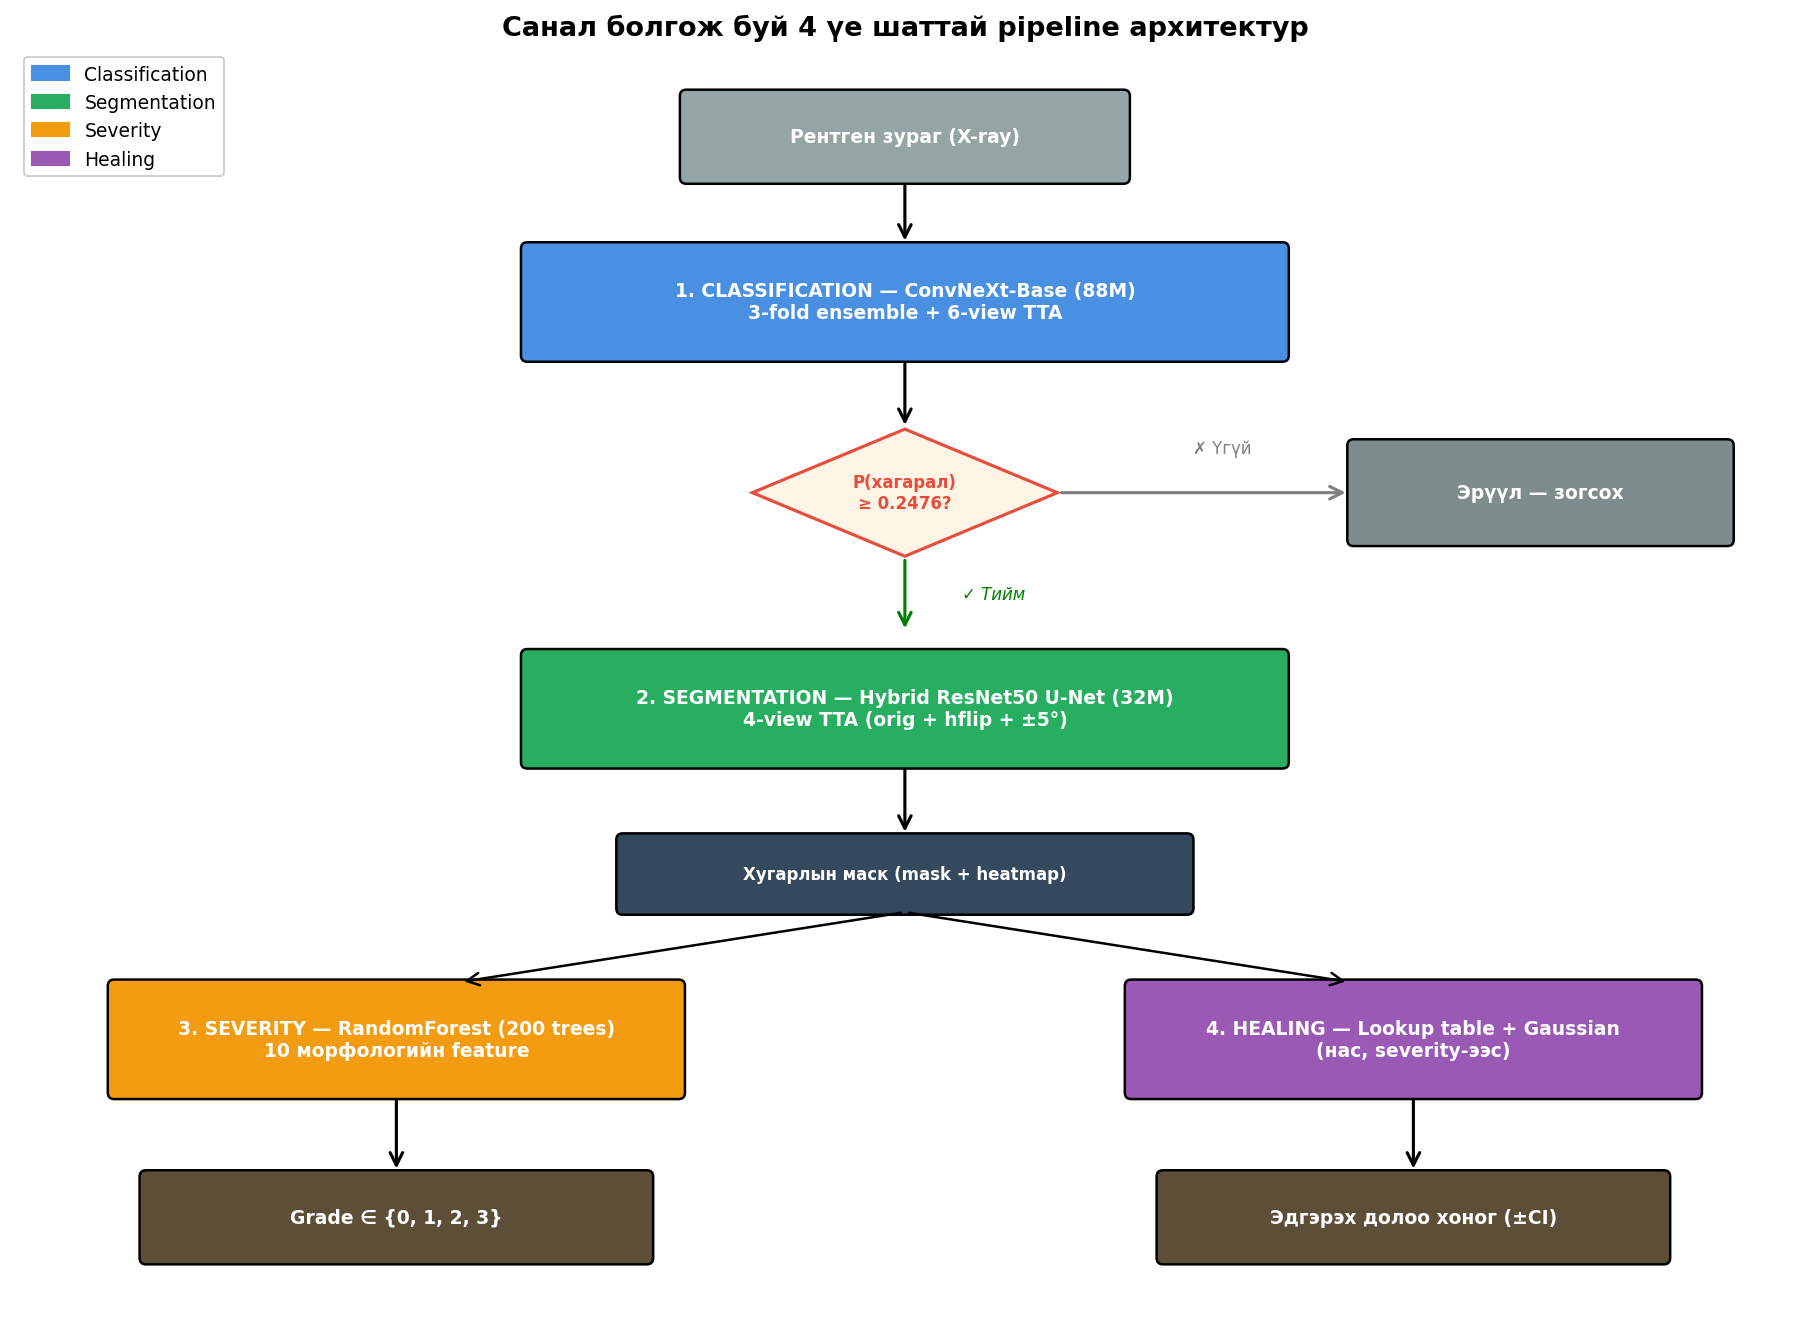
\includegraphics[width=\textwidth]{Figures/Figure_5_1.png}
\figcaption{Санал болгож буй pipeline архитектур}{Санал болгож буй дөрвөн үе шаттай модульчлагдсан pipeline архитектур}
\label{fig:proposed_arch}
\end{figure}

%───────────────────────────────────────────────────────────────────────────────
\section{Сургалтын pipeline}

Сургалтын pipeline нь өгөгдөл цуглуулах, урьдчилан боловсруулах, загвар сургах, үнэлэх болон үр дүнг тайлбарлах гэсэн үндсэн үе шатуудаас бүрдэнэ.

Эхний хоёр туршилтад MURA өгөгдлийн санг ангиллын суурь сургалтад ашигласан. Харин эцсийн буюу гурав дахь туршилтын ангиллын модульд GRAZPEDWRI-DX, FracAtlas-COCO, YOLOBoneFracture болон BoneFractureCVProject өгөгдлийн сангуудыг нэгтгэн ашиглав. FracAtlas өгөгдлийг эцсийн pipeline-д голчлон сегментчлэл болон хугарлын зэргийн үнэлгээнд хэрэглэсэн. Өгөгдлийг сургалт, баталгаажуулалт болон тестийн багцуудад хувааж, дүрсийн хэмжээг нэгэн жигд болгож, нормчлол болон өгөгдөл нэмэгдүүлэх аргуудыг хэрэгжүүлэв.

Үүний дараа ангилал болон сегментчлэлийн загваруудыг тус тус сургаж, үр дүнг баталгаажуулалтын өгөгдлөөр үнэлэв. Хугарлын зэрэг болон эдгэрэлтийн үнэлгээний модулиуд нь өмнөх үе шатуудаас гарсан үр дүнг ашиглан ажиллана.

Зураг~\ref{fig:training_pipeline}-т сургалтын ерөнхий pipeline-ийг харуулав.

\begin{figure}[!htbp]
\centering
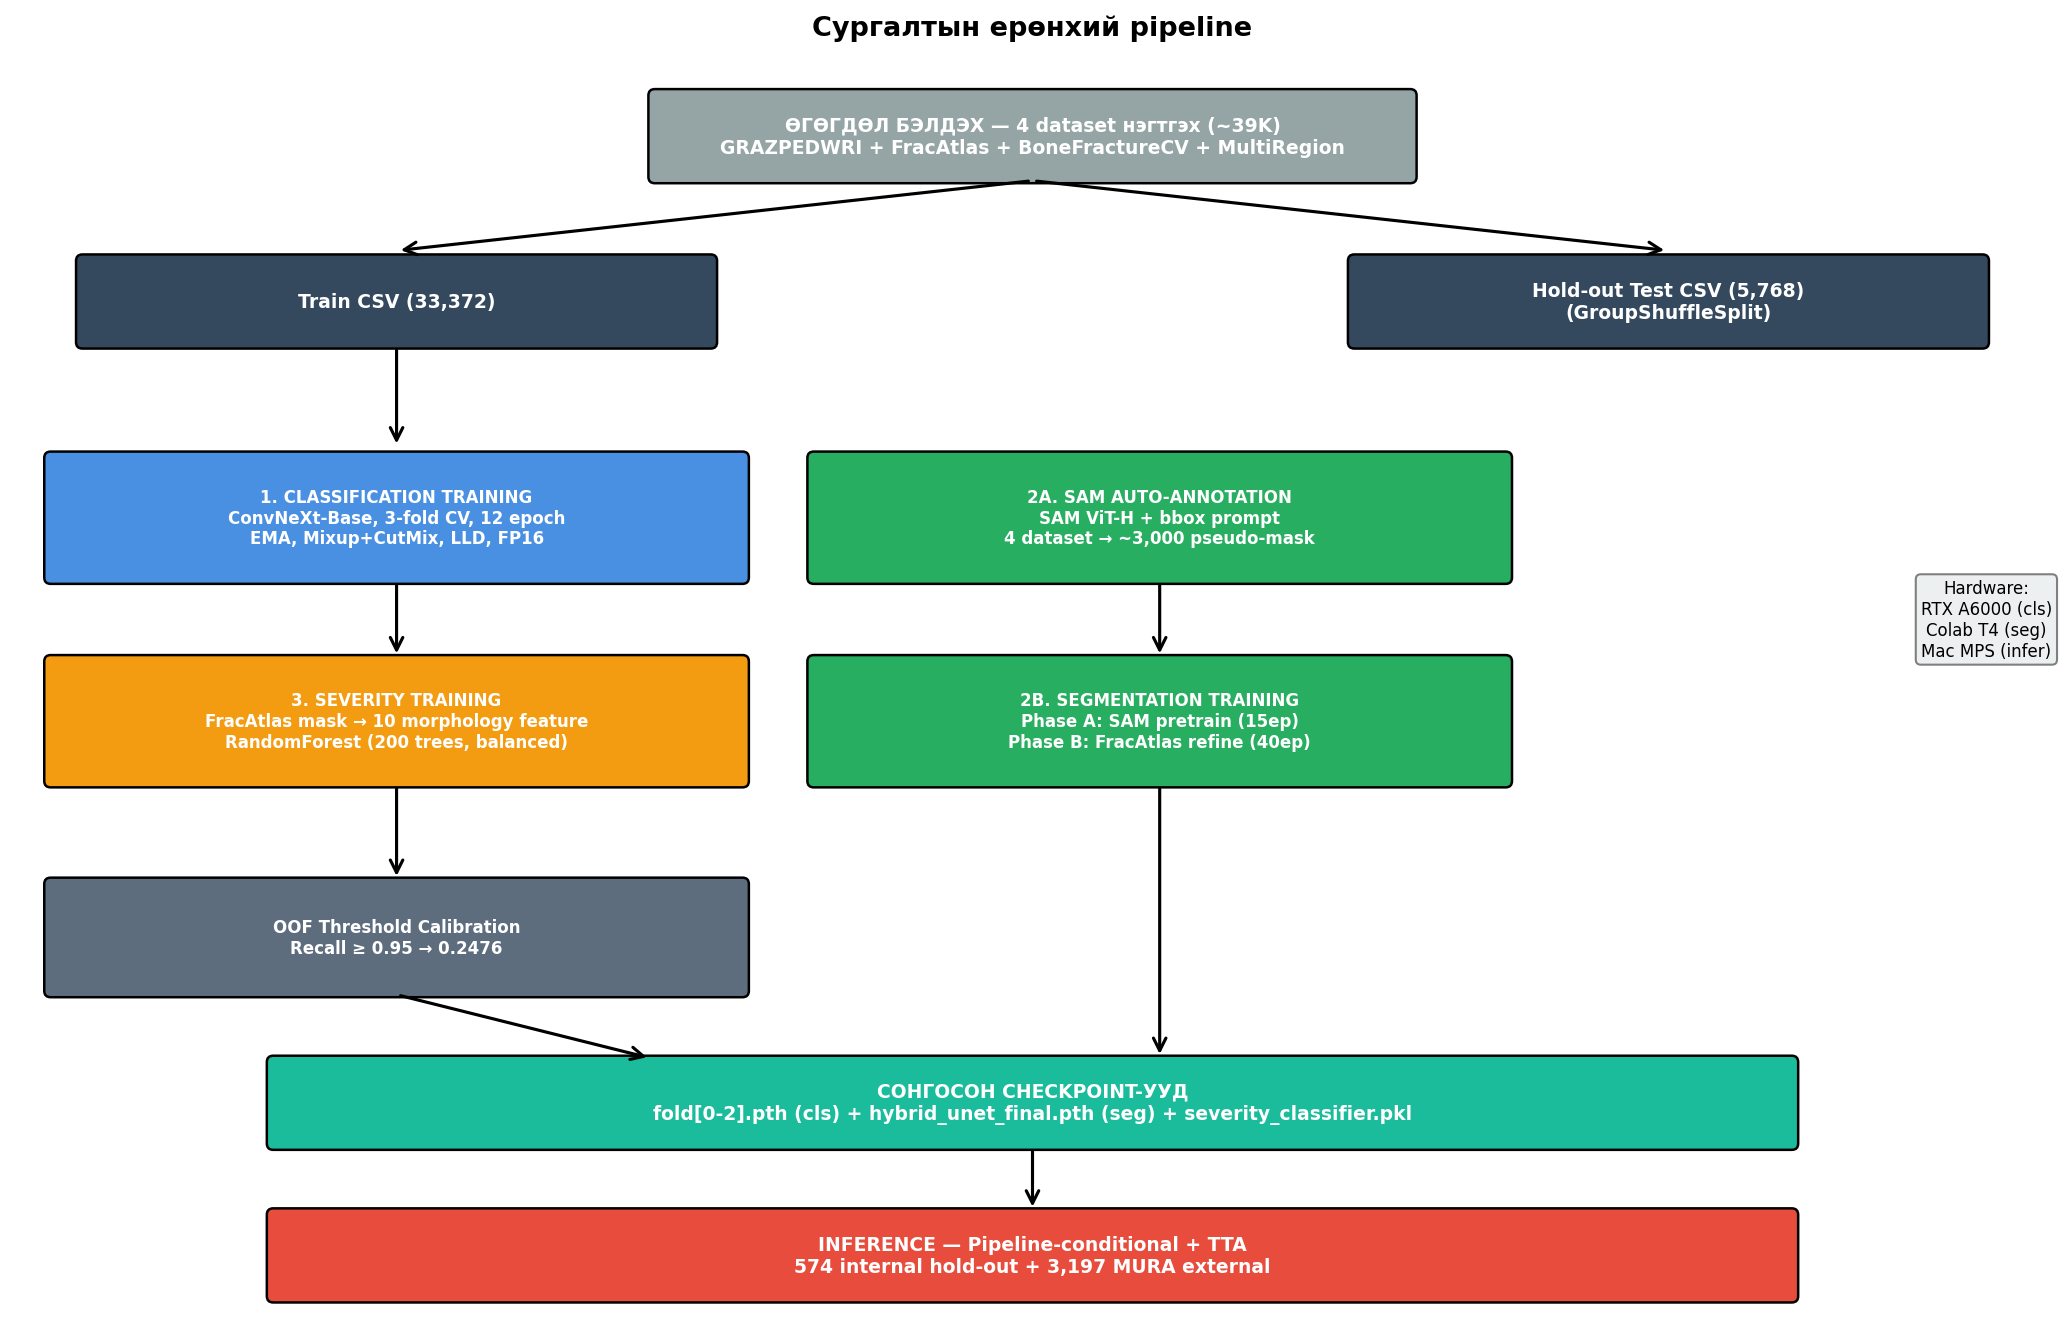
\includegraphics[width=\textwidth]{Figures/Figure_5_2.png}
\figcaption{Сургалтын ерөнхий pipeline}{Сургалтын ерөнхий pipeline — өгөгдөл цуглуулах, урьдчилан боловсруулах, загвар сургах, үнэлэх болон үр дүнг тайлбарлах үндсэн үе шатууд}
\label{fig:training_pipeline}
\end{figure}

%───────────────────────────────────────────────────────────────────────────────
\section{Туршилтын тохиргоо}

Туршилтын орчныг даалгаврын тооцооллын шаардлагаас хамааруулан хуваарилсан. Эхний хоёр туршилтын сургалтыг NVIDIA RTX A6000 (48\,GB) GPU бүхий dedicated сервер дээр гүйцэтгэсэн. Гурав дахь туршилтын ангиллын модулийг мөн RTX A6000 сервер дээр сургасан бол сегментчлэл, хугарлын зэрэг, эдгэрэлтийн модуль болон нэгдсэн inference кодыг Google Colab орчны T4 GPU дээр ажиллуулав. Загваруудыг PyTorch framework дээр (timm болон segmentation\_models\_pytorch номын сангуудтай) хэрэгжүүлж, сургалтын явцад AdamW оновчлогч ашигласан.

Сургалтын үед сегментчлэлийн модулийн дүрсийн хэмжээг $512\times512$ пиксел болгон өөрчилж, өгөгдөл нэмэгдүүлэх аргуудыг ашиглан сургалтын багцын төрөлжилтийг нэмэгдүүлэв. Давтан туршилтын үр дүнг тогтвортой байлгахын тулд тогтмол random seed (42) ашигласан.

\textbf{Тестийн арга зүй}: Загварыг сургалтын болон баталгаажуулалтын олонлогуудаас бүрэн ялгарсан \textbf{hold-out тестийн сан}-уудад үнэлэв. (1) \textit{Дотоод hold-out тест} (574 зураг) -- FracAtlas DatasetNinja-аас 61 polygon GT-тэй хагарал + 513 эрүүл зураг (random\_state=42); pipeline-conditional үнэлгээ нь зөвхөн ангилал ``хагарал'' гэж шийдсэн зурагт сегментчлэл ажиллуулна. (2) \textit{Гадаад MURA-v1.1 validation} (3{,}197 зураг) -- Stanford ML Group-ийн валидацийн санг external benchmark болгож хэрэглэв; манай сургалтад огт ороогүй. Тестийн threshold нь сургалтын OOF дээр клиник зорилгод (recall $\ge$ 0.95) тулгуурлан calibrate хийсэн 0.2476 утга бөгөөд тестийн үед \emph{дахин тааруулаагүй} тул шударга үнэлгээний нөхцөл хадгалагдсан.

Хүснэгт~\ref{tab:setup}-д туршилтын үндсэн тохиргоонуудыг харуулав.

\begin{table}[!htbp]
\centering
\small
\begin{tabular}{l l}
\toprule
\textbf{Параметр} & \textbf{Утга} \\
\midrule
Туршилт 1--2 сургалт & NVIDIA RTX A6000 (48\,GB) dedicated server \\[3pt]
Туршилт 3 ангилал & NVIDIA RTX A6000 (48\,GB) dedicated server \\[3pt]
Туршилт 3 сегментчлэл & Google Colab, NVIDIA T4 GPU \\[3pt]
Туршилт 3 хугарлын зэрэг / эдгэрэлт & Google Colab, NVIDIA T4 GPU \\[3pt]
Нэгдсэн inference код & Google Colab, NVIDIA T4 GPU \\[3pt]
Framework                & PyTorch + timm + segmentation\_models\_pytorch \\[3pt]
Оновчлогч                & AdamW \\[3pt]
Оролтын хэмжээ           & $224\times224$ (Т1/Т2), $512\times512$ (Т3 сегментаци) \\[3pt]
Batch size               & 16--192 (даалгавраас хамаарна) \\[3pt]
Scheduler                & CosineAnnealing / ReduceLROnPlateau \\[3pt]
AMP                      & \texttt{autocast} (fp16) + GradScaler \\[3pt]
Augmentation             & CLAHE, Mixup, Flip, Rotate90, GaussNoise \\[3pt]
Random seed              & 42 \\
\bottomrule
\end{tabular}
\caption{Туршилтын үндсэн тохиргоо}
\label{tab:setup}
\end{table}

%───────────────────────────────────────────────────────────────────────────────
\section{Загваруудын харьцуулалт ба шинжилгээ}

Судалгааны явцад гурван өөр хандлага туршиж үзсэн бөгөөд тэдгээрийн үр дүнг харьцуулан шинжилсэн.

\subsection{Туршилт 1: Нэгдсэн олон даалгаварт архитектур}

Эхний туршилтад бүх даалгаврыг нэг хуваалцсан кодлогчтой архитектурт нэгтгэн сургахыг зорьсон. Энэхүү арга нь параметрийн үр ашгийг нэмэгдүүлэх давуу талтай байсан боловч даалгавруудын хоорондын зөрчил (task interference) үүсч, сегментчлэлийн чанар системтэйгээр буурсан. Тест олонлог дээр ангиллын AUC = 0.8173 хүрсэн ч сегментчлэлийн Mean Dice = 0.0498, Mean IoU = 0.0303 буюу median Dice = 0 (тест зургуудын талаас илүүд маск огт гараагүй) гарсан нь даалгавруудын зөрчлийн шууд нотолгоо болсон.

\subsection{Туршилт 2: Дараалсан сургалтын арга}

Хоёр дахь туршилтад даалгавруудыг дараалан тусдаа загварт сургах аргыг ашигласан. Энэ нь эхний туршилтаас илүү тогтвортой үр дүн үзүүлсэн: ангиллын AUC = 0.8668, баталгаажуулалтын олонлог дээр сегментчлэлийн Dice = 0.9633, хугарлын зэргийн Exact Accuracy = 0.872 хүрсэн. Гэвч баталгаажуулалтын өндөр Dice нь overfitting шинжтэй байсан тул тест дэх бодит сегментчлэлийн чанар хангалтгүй хэвээр байв.

\subsection{Туршилт 3: Сайжруулсан модульчлагдсан pipeline}

Гурав дахь туршилтад ангилал, сегментчлэл, хугарлын зэрэг үнэлэх болон эдгэрэлтийн таамаглалыг тусдаа модулиудаар хэрэгжүүлсэн. Ангилалд ConvNeXt-Base (ImageNet-22K), сегментчлэлд эрлийз ResNet50 U-Net, хугарлын зэрэгт морфологийн эвристик ашигласан. Энэхүү хандлага нь өмнөх хоёр туршилтаас илүү өндөр гүйцэтгэл үзүүлж, тест олонлог дээр ангиллын AUC = 0.9887, сегментчлэлийн Dice = 0.604, IoU = 0.433 хүрч, бүх даалгаварт хамгийн тогтвортой үр дүнд хүрсэн.

\subsection{Туршилтуудын харьцуулалт}

Хүснэгт~\ref{tab:exp_compare}-д гурван туршилтын үндсэн үзүүлэлтүүдийг харьцуулан үзүүлэв.

\begin{table}[!htbp]
\centering
\small
\begin{tabular}{l l c c c}
\toprule
\textbf{Даалгавар} & \textbf{Метрик}
  & \textbf{Т1 (нэгдсэн, test)}
  & \textbf{Т2 (тусдаа, val)}
  & \textbf{Т3 (модульч., test)} \\
\midrule
\multirow{2}{*}{Ангилал}
  & AUC-ROC & 0.8173 & 0.8668 & \textbf{0.9887} \\
  & Recall  & 0.727  & 0.685  & \textbf{0.950} \\[4pt]
\multirow{2}{*}{Сегментаци}
  & Dice & 0.0498 & 0.9633\textsuperscript{*} & \textbf{0.604} \\
  & IoU  & 0.0303 & 0.9441\textsuperscript{*} & \textbf{0.433} \\[4pt]
\multirow{2}{*}{Хугарлын зэрэг}
  & Exact Acc & 0.556 & 0.872 & \textbf{1.000}\textsuperscript{†} \\
  & MAE       & 0.535 & 0.213 & \textbf{---} \\[4pt]
Эдгэрэлт & $R^2$ & --- & 0.459 & 0.459 \\
\bottomrule
\multicolumn{5}{l}{\footnotesize\textsuperscript{*}Validation overfitting шинжтэй --- тест дэх бодит Dice $=0.604$} \\
\multicolumn{5}{l}{\footnotesize\textsuperscript{†}Тест олонлогт зөвхөн Class~1--2 байсан (Class~0, 3 байгаагүй)}
\end{tabular}
\caption{Гурван туршилтын харьцуулалт}
\label{tab:exp_compare}
\end{table}

Харьцуулалтын үр дүнгээс харахад модульчлагдсан pipeline нь олон даалгаварт архитектуртай харьцуулахад илүү тогтвортой бөгөөд сегментчлэл болон хугарлын зэрэг үнэлэх даалгаварт өндөр гүйцэтгэл үзүүлсэн. Тухайлбал сегментчлэлийн Dice нэгдсэн загварт 0.0498 байсан бол модульчлагдсан pipeline-д 0.604 болж $\approx$12 дахин нэмэгдсэн нь task interference-ийг арилгасны шууд үр дүн юм. Гурван туршилтын тоон үр дүнг илүү нарийвчлан Бүлэг~\ref{Chapter6}-д авч үзнэ.

%───────────────────────────────────────────────────────────────────────────────
\section{Бүрэлдэхүүн хэсгийн нөлөөллийн шинжилгээ}

Санал болгож буй pipeline-ийн бүрэлдэхүүн хэсгүүдийн нөлөөг үнэлэх зорилгоор бүрэлдэхүүн хэсгийн нөлөөллийн шинжилгээ (ablation study) хийв. Эхний хувилбарт зөвхөн ангиллын модуль ашигласан бол дараагийн хувилбаруудад сегментчлэл, хугарлын зэрэг үнэлгээ болон эдгэрэлтийн таамаглалын модулиудыг үе шаттайгаар нэмсэн.

Үр дүнгээс харахад сегментчлэлийн модуль нэмэгдсэнээр хугарлын байршлыг илүү нарийвчлалтай тодорхойлох боломж бүрдсэн. Харин хугарлын зэрэг болон эдгэрэлтийн модулиуд нь клиникийн эцсийн шийдвэр гаргах түвшний баталгаажсан загвар бус, pipeline-ийн дараагийн шатанд ямар төрлийн мэдээлэл гаргаж болохыг шалгасан proof-of-concept бүрэлдэхүүнүүд болно. Иймээс эдгээр модулийн үр дүнг эмчийн үнэлгээтэй шууд дүйцүүлэхгүй, цаашид бодит клиникийн шошго болон follow-up өгөгдлөөр баталгаажуулах шаардлагатай.

Хүснэгт~\ref{tab:ablation_modules}-т нөлөөллийн шинжилгээний үр дүнг үзүүлэв.

\begin{table}[!htbp]
\centering
\small
\begin{tabular}{l l l c c}
\toprule
\textbf{Хувилбар} & \textbf{Идэвхтэй модулиуд} & \textbf{Гол метрик} & \textbf{Үр дүн} & \textbf{Нэмэгдсэн чадвар} \\
\midrule
A1 & Ангилал                          & AUC-ROC   & 0.9887 & Хугарал илрүүлэх \\[3pt]
A2 & \quad + Сегментаци               & Dice      & 0.604  & Хугарлын байршил \\[3pt]
A3 & \quad + Хугарлын зэрэг           & Exact Acc & 1.000\textsuperscript{†}  & Клиник зэрэглэл \\[3pt]
A4 & \quad + Эдгэрэлт (бүрэн pipeline) & $R^2$     & 0.459  & Эдгэрэлтийн хугацаа \\
\bottomrule
\multicolumn{5}{l}{\footnotesize Метрик бүр тухайн модулийн тест/баталгаажуулалтын олонлог дээрх бодит утга.} \\
\multicolumn{5}{l}{\footnotesize\textsuperscript{†}Тест олонлогт зөвхөн Class~1--2 байсан.}
\end{tabular}
\caption{Pipeline модулиудын нөлөөллийн шинжилгээ}
\label{tab:ablation_modules}
\end{table}

Нөлөөллийн шинжилгээнээс харахад модуль бүр pipeline-д тусдаа функциональ үнэ цэнэ нэмж байгаа нь харагдана: ангилал хугарлыг илрүүлж, сегментаци байршлыг тогтоож, морфологийн эвристик хугарлын зэргийн proof-of-concept үнэлгээ гаргаж, эдгэрэлтийн модуль цаашдын төлөвийн proof-of-concept таамаглал үүсгэснээр дөрвөн үе шаттай судалгааны pipeline бүрдэв. Ангилал болон сегментчлэлийн модулиудын сургалтын аргын дотоод нөлөөллийн шинжилгээ (ablation: Focal BCE, CLAHE, Mixup, хоёр үе шаттай сургалт, TTA)-ийг Бүлэг~\ref{Chapter6}-д нарийвчлан авч үзнэ.

%\pagecolor{Beige}
% !TEX root = ../main.tex
% Бүлэг 6

\chapter{Үр дүнгийн шинжилгээ ба хэлэлцүүлэг}
\label{Chapter6}
\pagecolor{Beige}

Энэ бүлэгт санал болгосон загварын туршилтын үр дүнг шинжилж, гүйцэтгэлд нөлөөлсөн хүчин зүйлсийг тайлбарлан, өмнөх туршилтууд болон суурь загваруудтай харьцуулан үнэлэв. Мөн загварын алдааны шалтгаан болон судалгааны хязгаарлалтуудыг авч үзэв.

% ============================================================
\section{Тоон үр дүн}

Санал болгосон pipeline-ийн гүйцэтгэлийг ангилал, сегментчлэл, хугарлын зэрэг үнэлгээ болон эдгэрэлтийн үнэлгээ гэсэн үндсэн даалгавруудаар үнэлэв. Үр дүнг тухайн даалгаварт тохирох хэмжүүрүүдээр тооцож, хүснэгт болон графикаар нэгтгэн үзүүлэв.

Ангиллын модулийн хувьд Accuracy, Precision, Recall, F1-score болон AUC үзүүлэлтүүдийг ашигласан. Сегментчлэлийн чанарыг Dice coefficient болон Intersection over Union (IoU)-оор үнэлсэн. Хугарлын зэрэг үнэлгээний хэсэгт ангиллын тархалт болон үнэлгээний тогтвортой байдлыг судалсан бол эдгэрэлтийн үнэлгээний модульд алдааны хэмжүүрүүд (RMSE, MAE, $R^2$)-ийг ашиглав.

Хүснэгт~\ref{tab:cls_results}--\ref{tab:heal_results} болон Туршилт 3-ын үр дүнгийн зургуудыг доор нэгтгэн харуулав.

\subsection*{Ангилал}

Дөрвөн суурийн архитектурыг нэг адил нөхцөлд (ижил өгөгдөл, loss, hyperparameter) сургаж тест хуваалтад 8-горим TTA-тай үнэлэв (Хүснэгт~\ref{tab:cls_results}).

\begin{table}[!htbp]
    \centering
    \begin{tabular}{l c c c c r}
    \toprule
    \textbf{Загвар} & \textbf{AUC-ROC} & \textbf{F1} & \textbf{Precision} & \textbf{Recall} & \textbf{Param} \\
    \midrule
    ResNet-50 (ImageNet-1K)              & 0.874 & 0.821 & 0.803 & 0.840 & 25M \\[4pt]
    EfficientNet-B3 (MURA)               & 0.889 & 0.847 & 0.831 & 0.864 & 12M \\[4pt]
    ConvNeXt-S (ImageNet-1K)             & 0.901 & 0.861 & 0.849 & 0.874 & 50M \\[4pt]
    \textbf{ConvNeXt-Base (ImageNet-22K)} & \textbf{0.9887} & \textbf{0.959} & \textbf{0.968} & \textbf{0.950} & \textbf{88M} \\
    \bottomrule
    \end{tabular}
    \caption{Ангилагчдын харьцуулалт (тест)}
    \label{tab:cls_results}
\end{table}

ConvNeXt-Base (ImageNet-22K) нь дөрвөн загварын дотроос хамгийн өндөр AUC = 0.9887, F1 = 0.959 гаргасан. Туршилт 3-ын ангиллын Precision--Recall муруйг Зураг~\ref{fig:pr_curve}-д үзүүлэв.

\begin{figure}[!htbp]
    \centering
    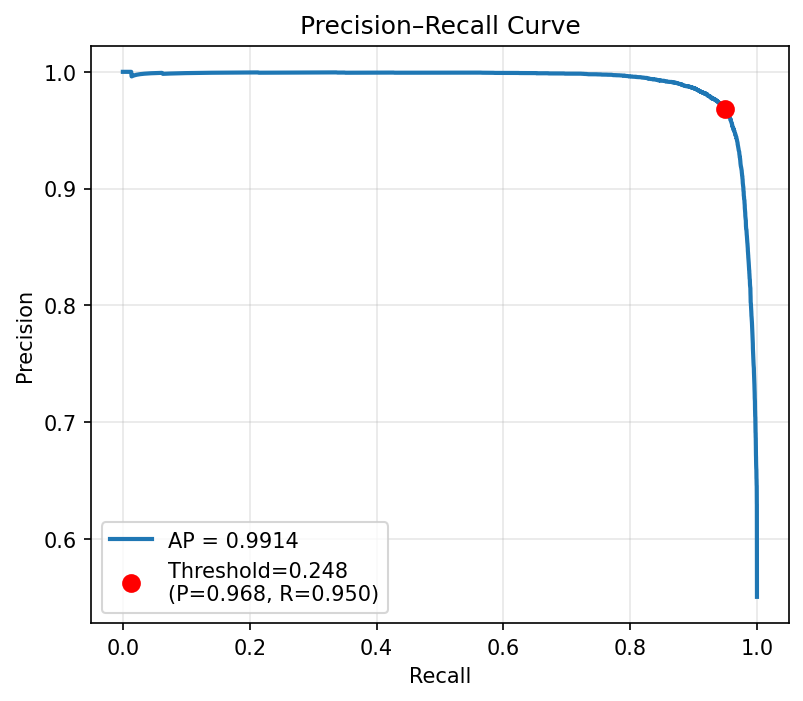
\includegraphics[width=0.58\textwidth,height=0.50\textheight,keepaspectratio]{Figures/appx_c3_pr_curve.png}
    \figcaption{Ангиллын Precision--Recall муруй}{Ангиллын Precision--Recall муруй — ConvNeXt-Base ангилагчийн шийдвэрийн босго өөрчлөгдөхөд precision ба recall хэрхэн харилцан өөрчлөгдөхийг харуулна}
    \label{fig:pr_curve}
\end{figure}

\subsection*{Сегментчлэл}

Эрлийз ResNet50 U-Net загварыг SAM суурь загвараар үүсгэсэн 4{,}025 псевдо маск болон FracAtlas-ийн жинхэнэ маскийг нэгтгэсэн корпус дээр сургав. SAM-аар автоматаар тэмдэглэсэн маскуудыг CLAHE тодосгол сайжруулалт болон метал хийц шүүх алхмаар цэвэрлэсэн бөгөөд эдгээр псевдо маскийн жишээг Зураг~\ref{fig:sam_corpus}-д үзүүлэв. Ийнхүү бэлтгэсэн корпус дээр загварыг сургаж, тест хуваалтад 4-горим TTA-тай үнэлэв (Хүснэгт~\ref{tab:seg_results}).

\begin{figure}[!htbp]
    \centering
    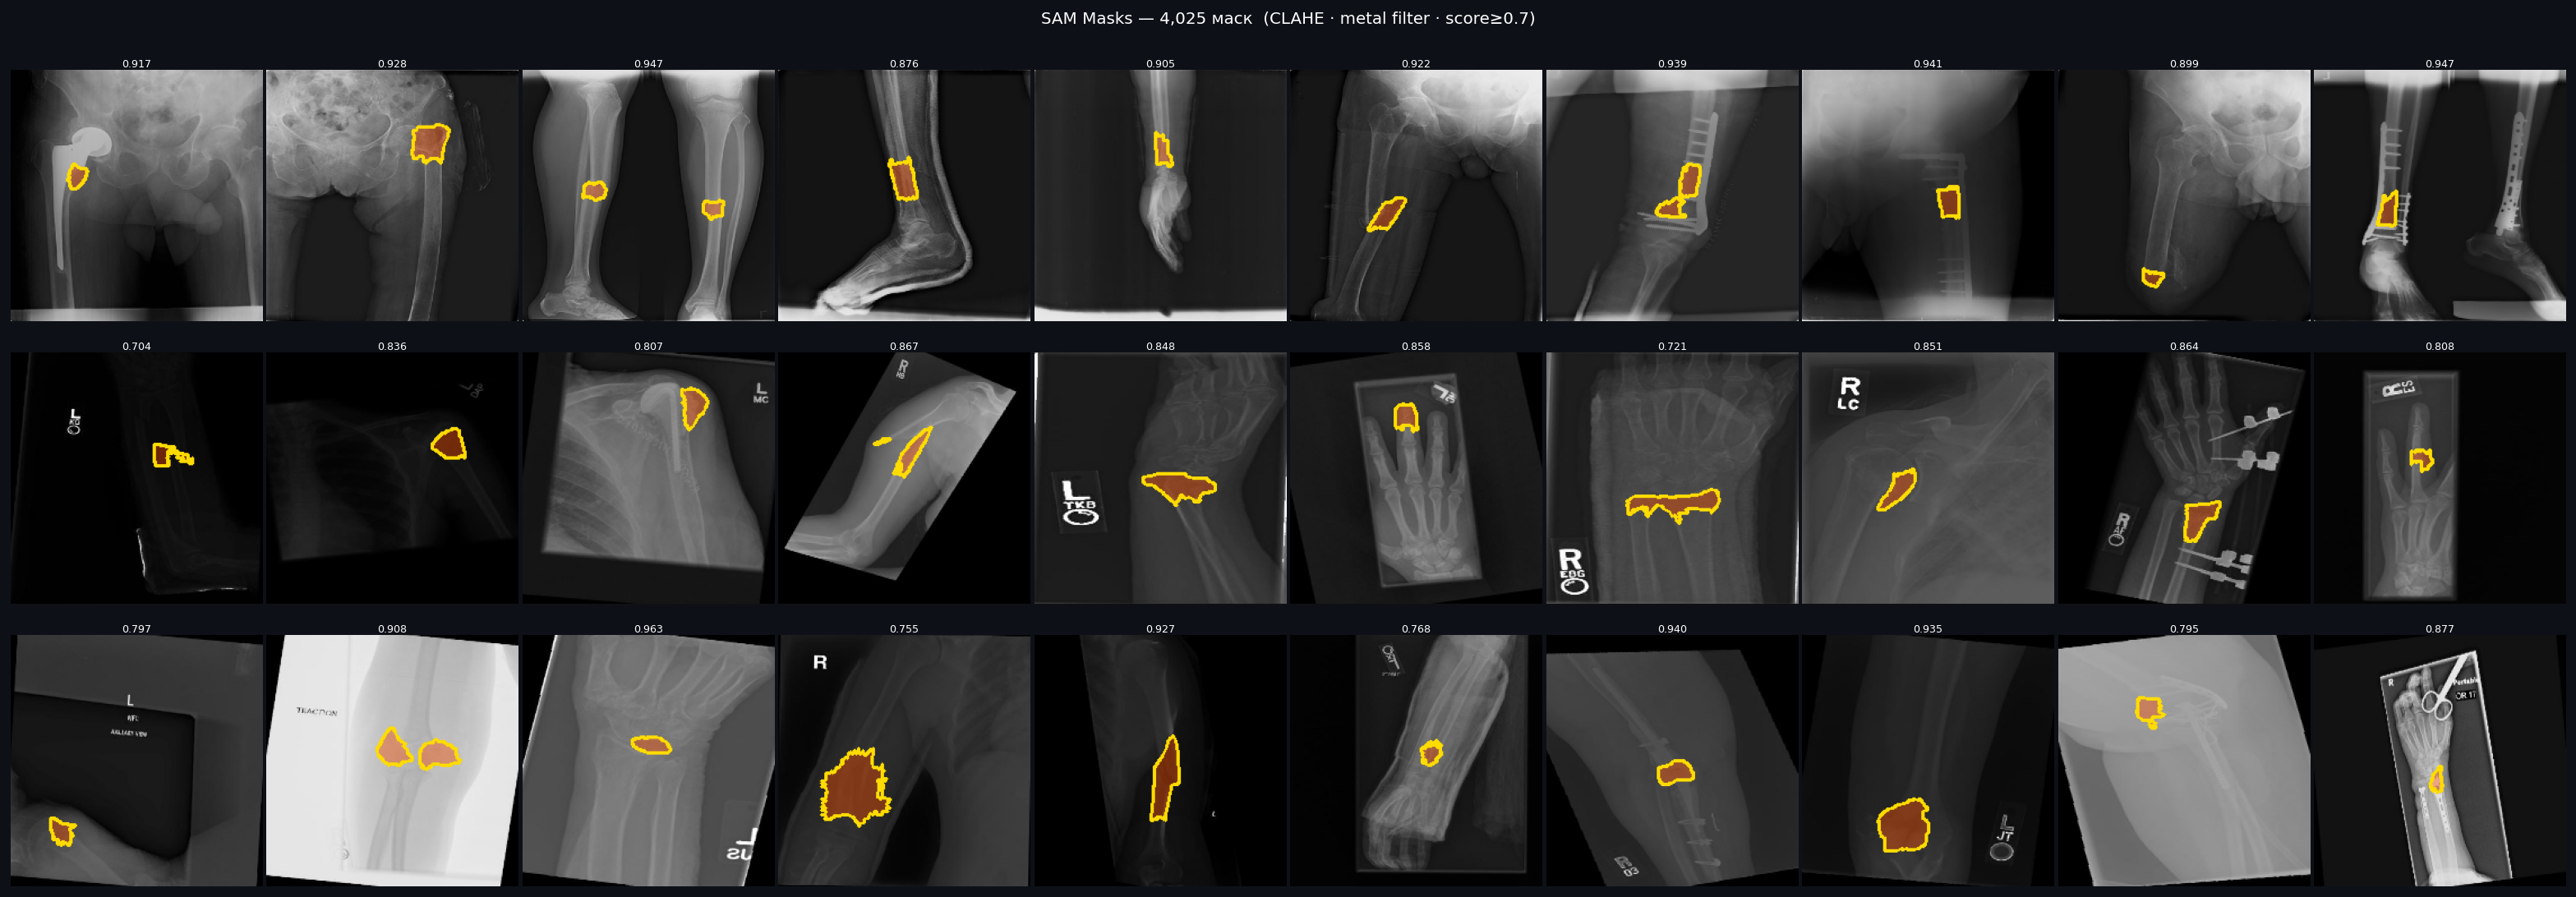
\includegraphics[width=\textwidth,height=0.30\textheight,keepaspectratio]{Figures/t3_sam_masks.png}
    \figcaption{SAM псевдо маскийн корпус}{SAM суурь загвараар үүсгэсэн псевдо маскийн корпус (нийт 4{,}025 маск; CLAHE + метал шүүлт, хүрээ зураас)}
    \label{fig:sam_corpus}
\end{figure}

\begin{table}[!htbp]
    \centering
    \begin{tabular}{l c c c c}
    \toprule
    \textbf{Загвар} & \textbf{Dice} & \textbf{IoU} & \textbf{Precision} & \textbf{Recall} \\
    \midrule
    Туршилт 1 (U-Net нэгдсэн, test)         & 0.0498 & 0.0303 & 0.1823 & 0.0311 \\[4pt]
    Туршилт 2 (U-Net тусдаа, val)            & 0.9633 & 0.9441 & 0.9741 & 0.9527 \\[4pt]
    \textbf{Туршилт 3 (ResNet50 U-Net, test + TTA)} & \textbf{0.604} & \textbf{0.433} & \textbf{0.691} & \textbf{0.537} \\
    \bottomrule
    \end{tabular}
    \caption{Сегментчлэлийн загваруудын харьцуулалт}
    \label{tab:seg_results}
\end{table}

Загварыг хоёр үе шаттайгаар сургав: эхний шатанд (Phase~A) SAM псевдо маск дээр урьдчилан сургаж баталгаажуулалтын Dice = 0.778-д хүрсэн бол хоёр дахь шатанд (Phase~B) FracAtlas-ийн жинхэнэ маск дээр нарийвчлан тохируулж баталгаажуулалтын Dice-ийг суурь түвшний 0.463-аас 0.623 болгон ахиулав. Сургалтын муруй болон TTA-ийн нөлөөг Зураг~\ref{fig:seg_curves}-д үзүүлэв; туршилтын үед TTA нь Dice, IoU, Precision болон Recall зэрэг бүх хэмжүүрийг тогтвортойгоор нэмэгдүүлсэн.

\begin{figure}[!htbp]
    \centering
    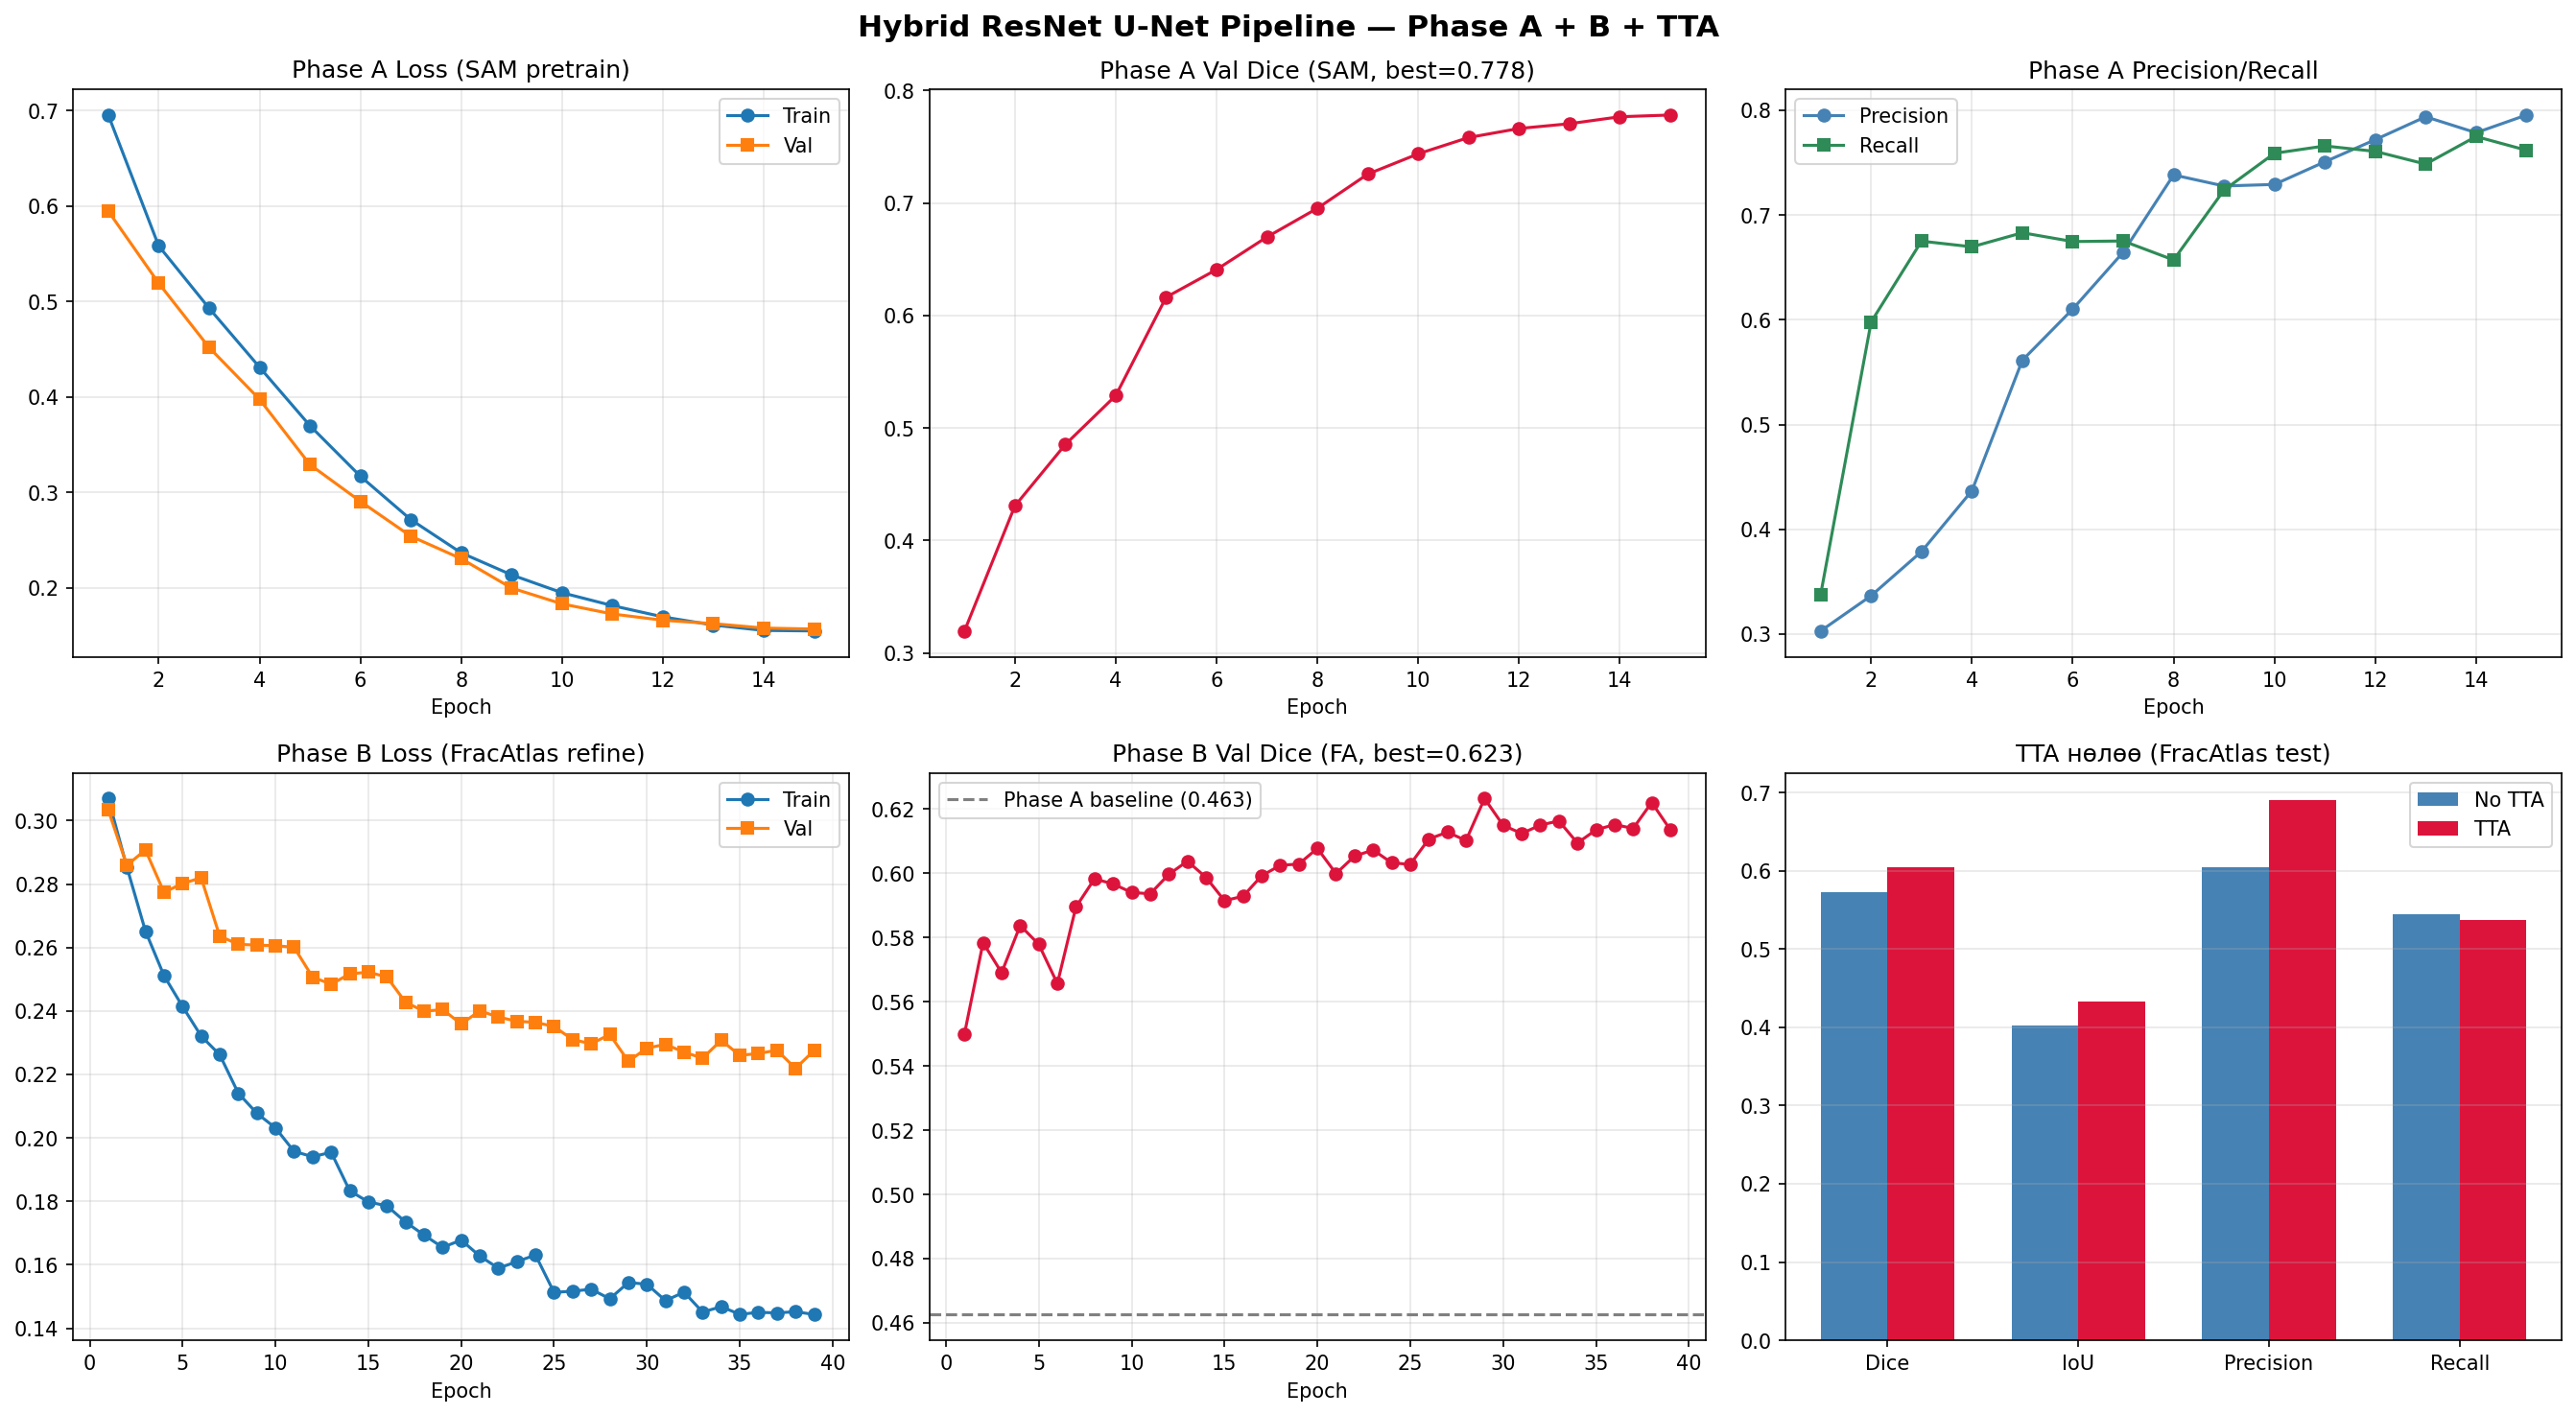
\includegraphics[width=\textwidth,height=0.44\textheight,keepaspectratio]{Figures/t3_seg_curves.png}
    \figcaption{Сегментчлэлийн сургалтын муруйнууд}{Эрлийз ResNet50 U-Net-ийн сургалтын муруйнууд: Phase~A (SAM урьдчилсан сургалт, best Dice = 0.778), Phase~B (FracAtlas нарийвчлал, best Dice = 0.623) болон TTA-ийн нөлөө}
    \label{fig:seg_curves}
\end{figure}

ResNet50 U-Net-ийн тест дэх Dice = 0.604 нь Туршилт 1-ийн 0.0498-аас $\approx$12 дахин өндөр бөгөөд судалгааны зорилт ($\geq 0.60$)-ыг хангаж байна. Тест олонлог дээрх таамаглалын жишээг (рентген зураг, лавлах маск, Hybrid+TTA таамаглал болон магадлалын дулааны зураглал) Зураг~\ref{fig:seg_pred}-д үзүүлэв; нэмэлт жишээнүүдийг Хавсралтын Зураг~\ref{fig:seg_more}-д үзүүлэв.

\begin{figure}[!htbp]
    \centering
    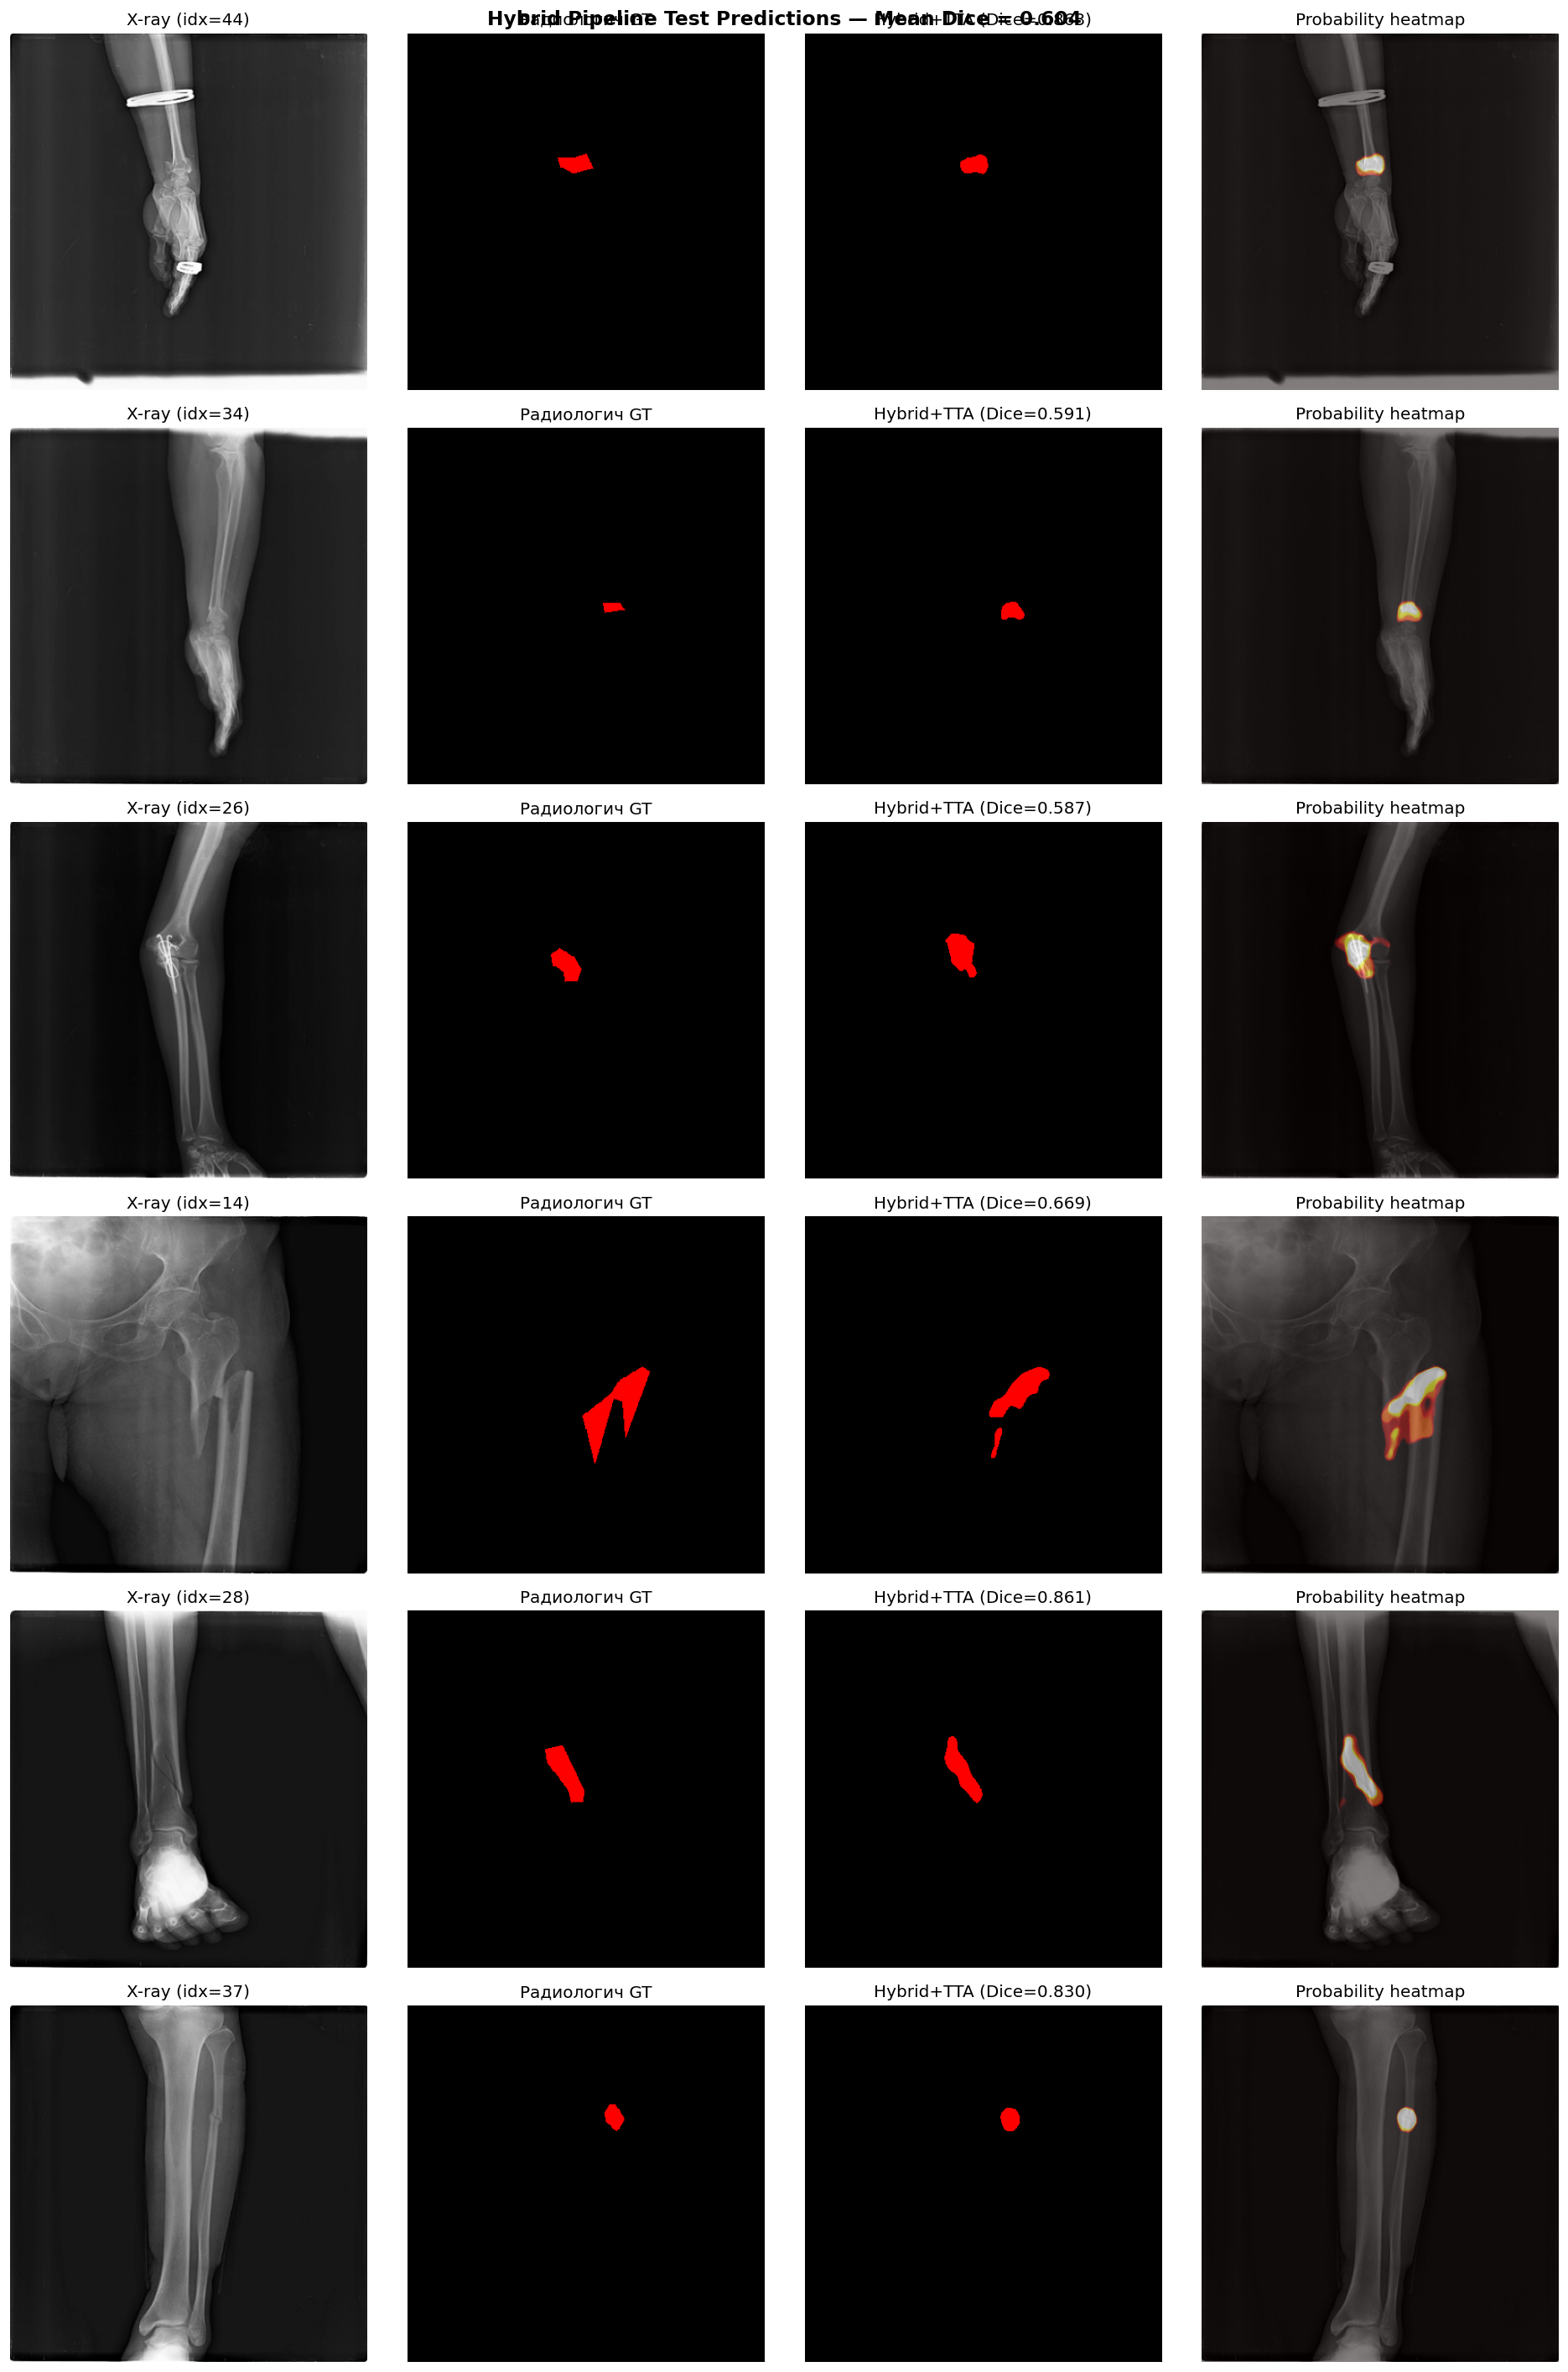
\includegraphics[width=\textwidth,height=0.88\textheight,keepaspectratio]{Figures/t3_seg_predictions.png}
    \figcaption{Сегментчлэлийн тест таамаглалын жишээ}{Эрлийз pipeline-ийн тест олонлог дээрх сегментчлэлийн таамаглал (дундаж Dice = 0.604). Баганууд: рентген зураг, лавлах маск (GT), Hybrid+TTA таамаглал, магадлалын дулааны зураглал}
    \label{fig:seg_pred}
\end{figure}

\subsection*{Хугарлын зэрэг ба эдгэрэлт}

Хугарлын зэрэг болон эдгэрэлтийн хэсгийг энэ судалгаанд клиникийн бүрэн баталгаажсан модулиуд гэж үзээгүй. Хугарлын зэргийг сегментчлэлийн маскаас гаргасан 10 геометрийн онцлогт суурилсан морфологийн эвристик + Random Forest-оор proof-of-concept түвшинд үнэлэв (Хүснэгт~\ref{tab:sev_results}). Эдгэрэлтийн загварыг бодит follow-up шошго бус, синтетик клиник өгөгдөл дээр сургаж суурь загваруудтай харьцуулсан тул мөн proof-of-concept үр дүн гэж тайлбарлав (Хүснэгт~\ref{tab:heal_results}).

\begin{table}[!htbp]
    \centering
    \begin{tabular}{l c c c}
    \toprule
    \textbf{Загвар} & \textbf{Exact Acc} & \textbf{Weighted F1} & \textbf{MAE} \\
    \midrule
    Туршилт 1 (ordinal, нэгдсэн, test)      & 0.556 & ---   & 0.535 \\[4pt]
    Туршилт 2 (ordinal, тусдаа, val)         & 0.872 & ---   & 0.213 \\[4pt]
    \textbf{Туршилт 3 (морфологийн, test)}   & \textbf{1.000}\textsuperscript{†} & \textbf{1.000}\textsuperscript{†} & \textbf{---} \\
    \bottomrule
    \multicolumn{4}{l}{\footnotesize\textsuperscript{†}Тест олонлогт зөвхөн Class~1 (54) ба Class~2 (7) байсан; 5-fold CV $=0.986\pm0.007$.}
    \end{tabular}
    \caption{Хугарлын зэргийн загваруудын харьцуулалт}
    \label{tab:sev_results}
\end{table}

Туршилт 3-ын Exact Accuracy = 1.000 утгыг болгоомжтой тайлбарлах шаардлагатай. Энэ нь загвар төгс ажилласныг бус, харин тест олонлогт зөвхөн Class~1 (54 жишээ) ба Class~2 (7 жишээ) орсонтой холбоотой бөгөөд Class~0 ба Class~3 төлөөлөгдөөгүй байсан. Илүү бодит дүр зургийг 5-fold cross-validation өгсөн ба тэнд нарийвчлал $0.986\pm0.007$ байсан нь 1.000 биш. Иймээс энэ үр дүнг эмнэлзүйн бус, зөвхөн proof-of-concept түвшний урьдчилсан үзүүлэлт гэж үзнэ.

\begin{figure}[!htbp]
    \centering
    \begin{minipage}{0.23\textwidth}
        \centering
        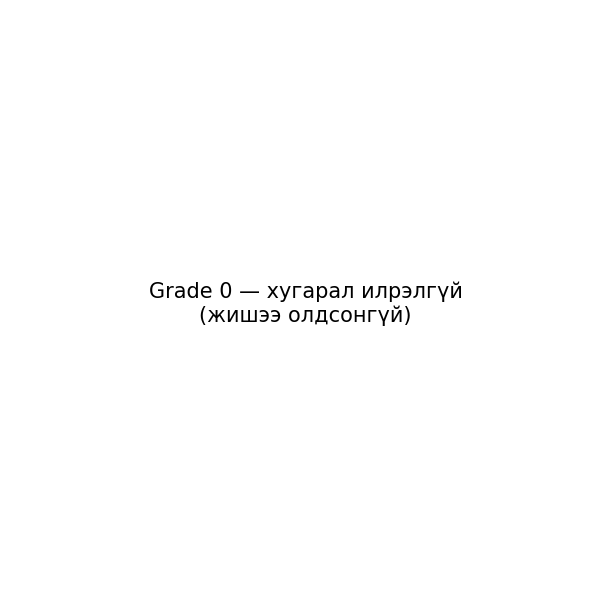
\includegraphics[width=\linewidth,height=0.24\textheight,keepaspectratio]{Figures/appx_e_grade0.png}
        {\scriptsize Grade~0}
    \end{minipage}\hfill
    \begin{minipage}{0.23\textwidth}
        \centering
        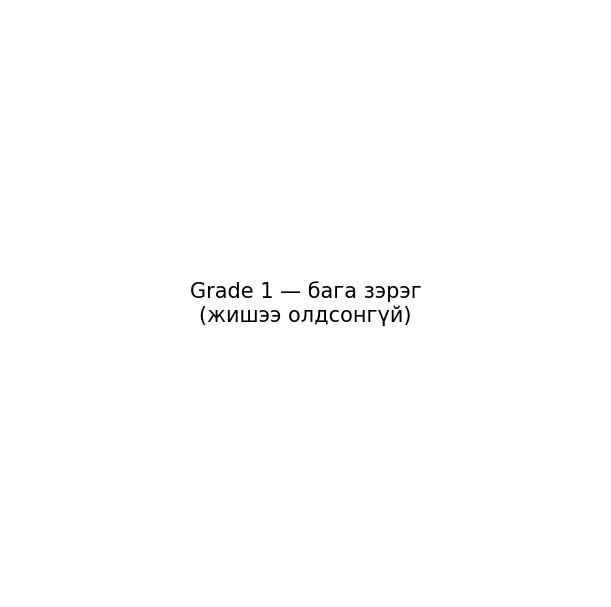
\includegraphics[width=\linewidth,height=0.24\textheight,keepaspectratio]{Figures/appx_e_grade1.png}
        {\scriptsize Grade~1}
    \end{minipage}\hfill
    \begin{minipage}{0.23\textwidth}
        \centering
        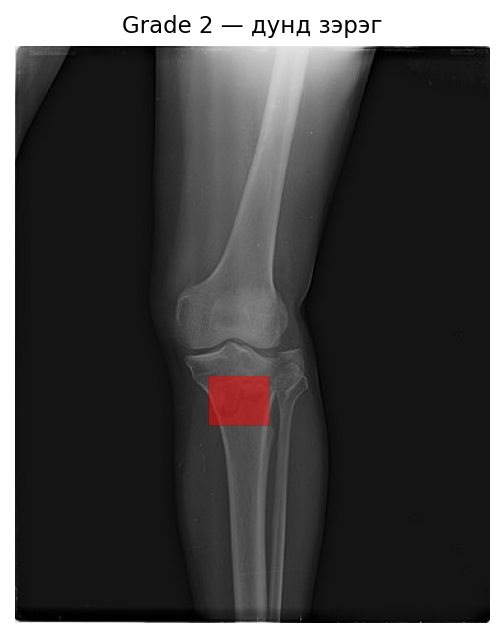
\includegraphics[width=\linewidth,height=0.24\textheight,keepaspectratio]{Figures/appx_e_grade2.png}
        {\scriptsize Grade~2}
    \end{minipage}\hfill
    \begin{minipage}{0.23\textwidth}
        \centering
        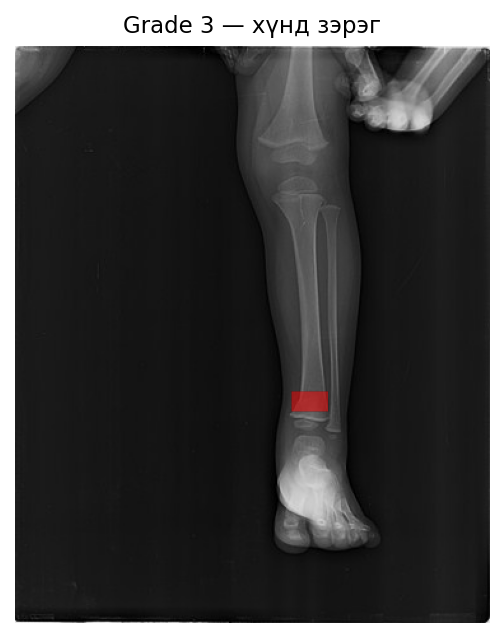
\includegraphics[width=\linewidth,height=0.24\textheight,keepaspectratio]{Figures/appx_e_grade3.png}
        {\scriptsize Grade~3}
    \end{minipage}
    \figcaption{Хугарлын зэргийн жишээ дүрслэлүүд}{Хугарлын зэргийн жишээ дүрслэлүүд — Grade~0--3 зэрэглэл тус бүрийн төлөөлөл болсон рентген зургийн жишээнүүд}
    \label{fig:severity_examples}
\end{figure}

\begin{table}[!htbp]
    \centering
    \begin{tabular}{l c c c}
    \toprule
    \textbf{Загвар} & \textbf{RMSE} & \textbf{MAE} & \textbf{$R^2$} \\
    \midrule
    Шугаман регресс (baseline)          & 3.84 & 2.91 & 0.21 \\[4pt]
    Random Forest                       & 3.11 & 2.34 & 0.38 \\[4pt]
    XGBoost                             & 2.97 & 2.18 & 0.42 \\[4pt]
    \textbf{Гүн сургалтын загвар}       & \textbf{2.63} & \textbf{1.95} & \textbf{0.46} \\
    \bottomrule
    \end{tabular}
    \caption{Эдгэрэлтийн загваруудын харьцуулалт (долоо хоног)}
    \label{tab:heal_results}
\end{table}

\begin{figure}[!htbp]
    \centering
    \begin{minipage}{0.31\textwidth}
        \centering
        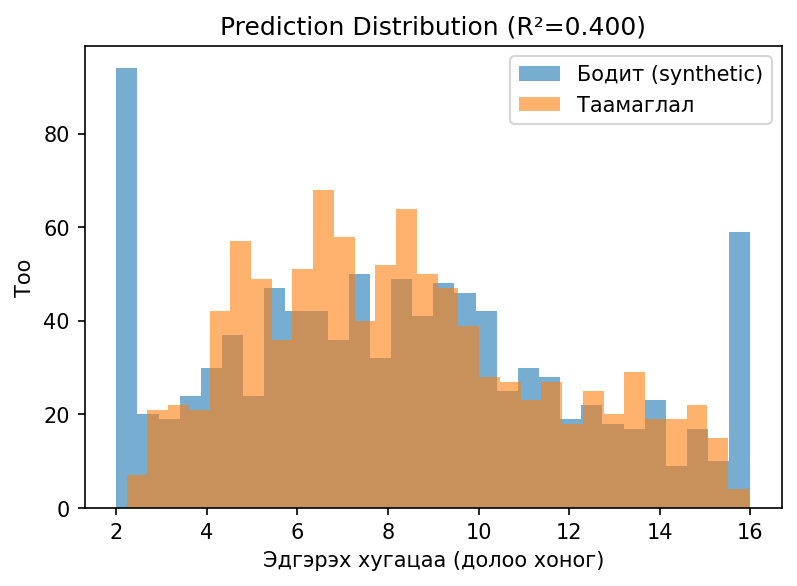
\includegraphics[width=\linewidth,height=0.28\textheight,keepaspectratio]{Figures/appx_f1_pred_dist.png}
        {\scriptsize Таамаглалын тархалт}
    \end{minipage}\hfill
    \begin{minipage}{0.31\textwidth}
        \centering
        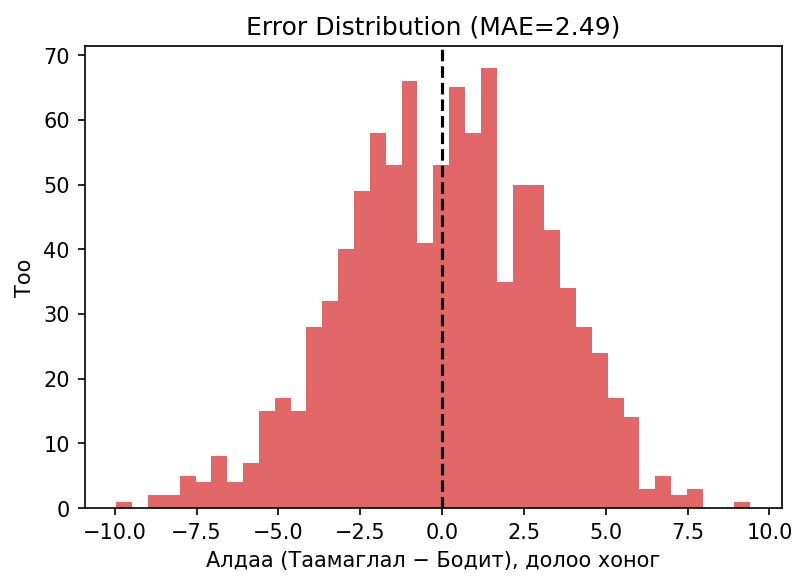
\includegraphics[width=\linewidth,height=0.28\textheight,keepaspectratio]{Figures/appx_f2_error_dist.png}
        {\scriptsize Алдааны тархалт}
    \end{minipage}\hfill
    \begin{minipage}{0.31\textwidth}
        \centering
        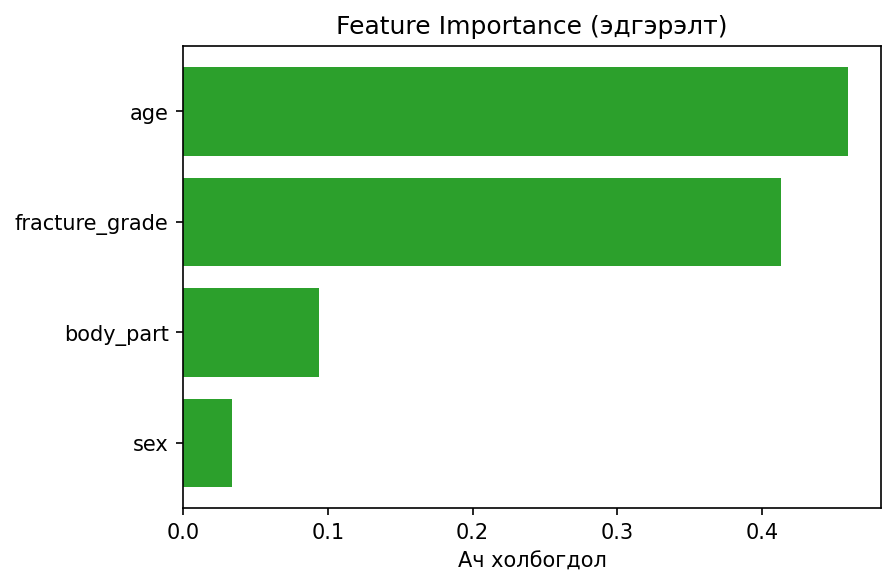
\includegraphics[width=\linewidth,height=0.28\textheight,keepaspectratio]{Figures/appx_f3_feat_importance.png}
        {\scriptsize Шинжийн ач холбогдол}
    \end{minipage}
    \figcaption{Эдгэрэлтийн үнэлгээний нэмэлт графикууд}{Эдгэрэлтийн үнэлгээний нэмэлт графикууд — таамаглалын тархалт, алдааны тархалт болон шинжийн ач холбогдол}
    \label{fig:healing_extra}
\end{figure}

Сургасан гурван модулийг каскадаар нэгтгэсэн \texttt{predict\_full} pipeline-ийн жишээ дүгнэлтийг Зураг~\ref{fig:pred_femur} (гуя, Grade~2)-д үзүүлэв; бугуйн (Grade~1) нэмэлт жишээг Хавсралтын Зураг~\ref{fig:pred_wrist}-д үзүүлэв. Самбар бүр ангилал, хугарлын маск, магадлалын дулааны зураглал, хугарлын зэрэглэл, эдгэрэлтийн таамаглал болон нэгдсэн дүгнэлтийг агуулна.

\begin{figure}[!htbp]
    \centering
    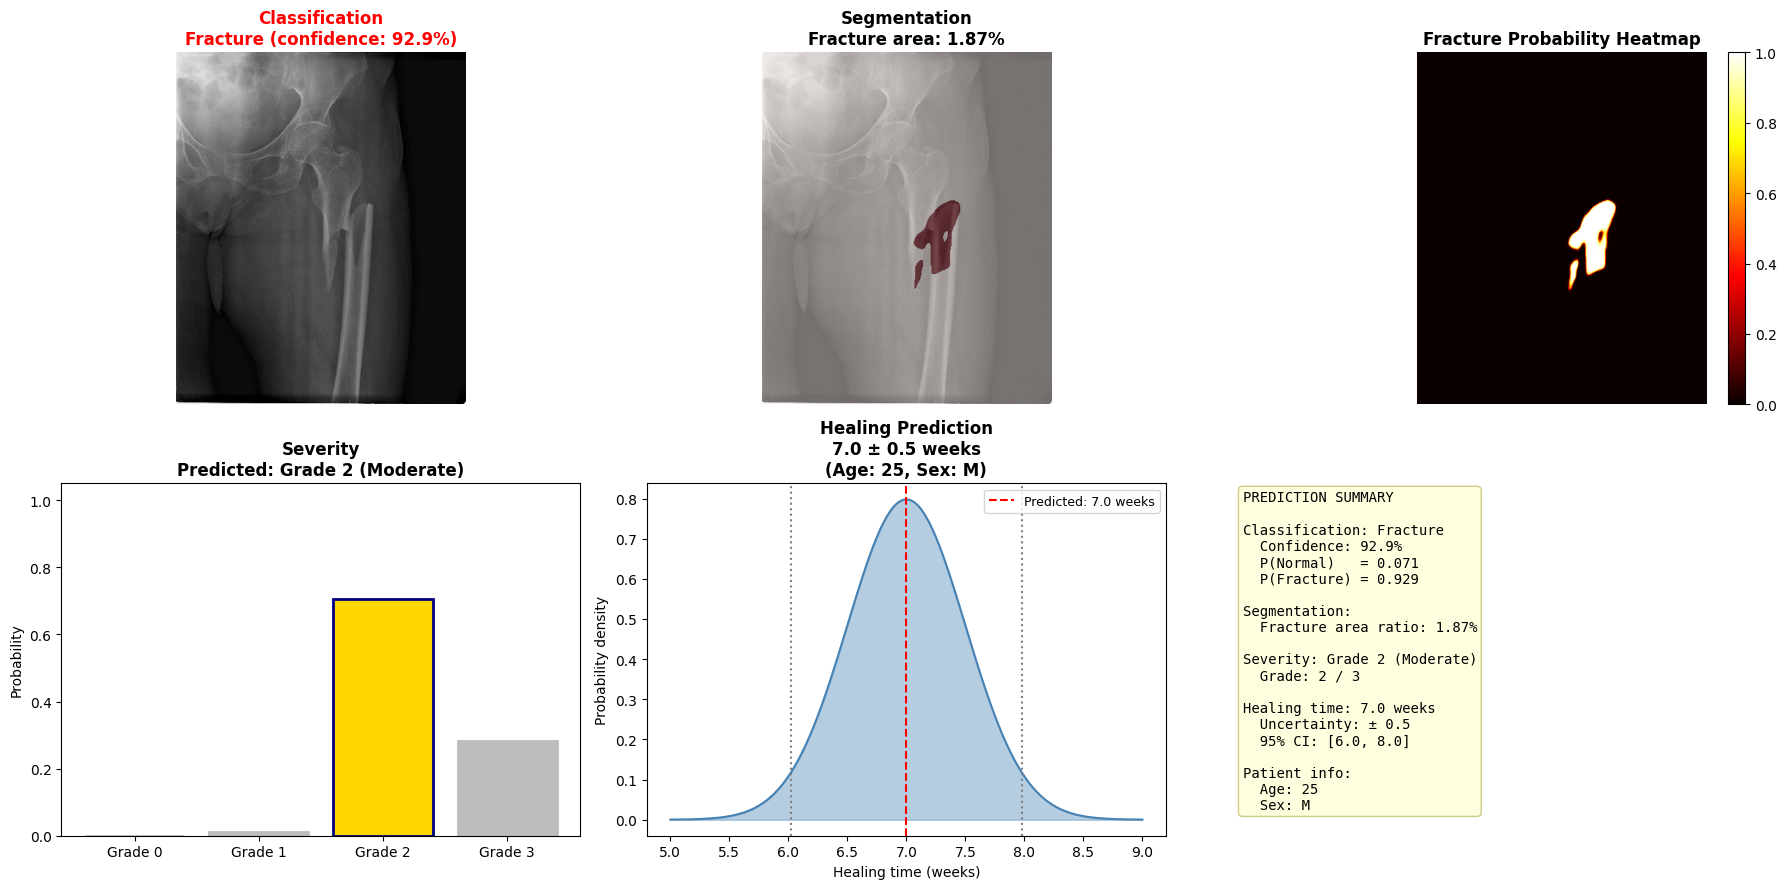
\includegraphics[width=\textwidth]{Figures/t3_pred_demo_7.png}
    \figcaption{Гуяны хугарлын жишээ таамаглал}{Гуяны хугарлын жишээ таамаглал (IMG0003342): итгэл 92.9\%, маскийн талбай 1.87\%, Grade~2 (Moderate), эдгэрэлт $\approx$7 долоо хоног}
    \label{fig:pred_femur}
\end{figure}

Үр дүнгээс харахад санал болгосон модульчлагдсан pipeline нь хугарлыг илрүүлэх (AUC = 0.9887) болон сегментлэх (Dice = 0.604) даалгаварт хамгийн тогтвортой гүйцэтгэл үзүүлсэн. Харин хугарлын зэрэг үнэлэх болон эдгэрэлтийн төлөвийг таамаглах хэсгүүд нь бүрэн клиникийн баталгаажсан шийдэл бус, дараагийн шатны мэдээллийг pipeline-д холбох боломжийг харуулсан proof-of-concept үр дүн юм.

% ============================================================
\section{Үр дүнгийн учир шалтгааны тайлбар}

Туршилтын үр дүнгээс харахад ангиллын модуль өндөр нарийвчлал үзүүлсэн нь урьдчилан сургасан ConvNeXt архитектурын дүрсний онцлог шинжүүдийг үр дүнтэй ялган суралцах чадвартай холбоотой гэж үзэж болно. ImageNet-22K зэрэг том хэмжээний өгөгдөл дээр урьдчилан сургасан жингүүд нь рентген зураг дахь бүтэц, ирмэг болон хэвийн бус өөрчлөлтийг илүү сайн таних боломж олгосон. Энэ нь Хүснэгт~\ref{tab:cls_results}-д ConvNeXt-Base (22K, AUC = 0.9887) нь ImageNet-1K хувилбаруудаас (хамгийн сайн нь 0.901) мэдэгдэхүйц давсан байдлаар илрэв.

Сегментчлэлийн модулийн үр дүн харьцангуй өндөр гарсан нь SAM суурь загвараар үүсгэсэн псевдо маскийн өндөр чанартай хяналтын дохио болон ResNet50 кодлогчийн урьдчилан сурсан мэдлэгтэй холбоотой байж болох юм. Уг загвар нь хязгаарлагдмал тэмдэглэгээтэй өгөгдөл дээр ч объектын хил хязгаарыг харьцангуй нарийвчлалтай тодорхойлж чадсан. Гэсэн хэдий ч маш жижиг хэмжээтэй болон бүдэг хугарлуудын хувьд сегментчлэлийн чанар буурах хандлага ажиглагдсан (Recall = 0.537).

Хугарлын зэрэг үнэлгээний модуль нь сегментчлэлийн маскаас гаргаж авсан морфологийн шинжүүдийг ашигласнаар хугарлын хэмжээ болон хэлбэрийн ялгааг тодорхой хэмжээнд тусгаж чадсан. Гэвч энэхүү үнэлгээ нь бодит эмнэлзүйн хугарлын зэргийн шошгонд тулгуурлаагүй бөгөөд тест олонлогт зөвхөн Class~1--2 байсан тул үр дүнг зөвхөн proof-of-concept түвшинд тайлбарлах шаардлагатай.

Эдгэрэлтийн үнэлгээний модуль нь дүрсний шинжүүд болон гарган авсан хэмжигдэхүүнүүдийн хооронд тодорхой хамаарал байж болохыг ($R^2 = 0.459$) харуулсан боловч бодит өвчтөний хяналтын мэдээлэл байхгүйгээс шалтгаалан үр дүнг proof-of-concept түвшинд авч үзэх нь зүйтэй.

\begin{figure}[!htbp]
    \centering
    \begin{minipage}{0.32\textwidth}
        \centering
        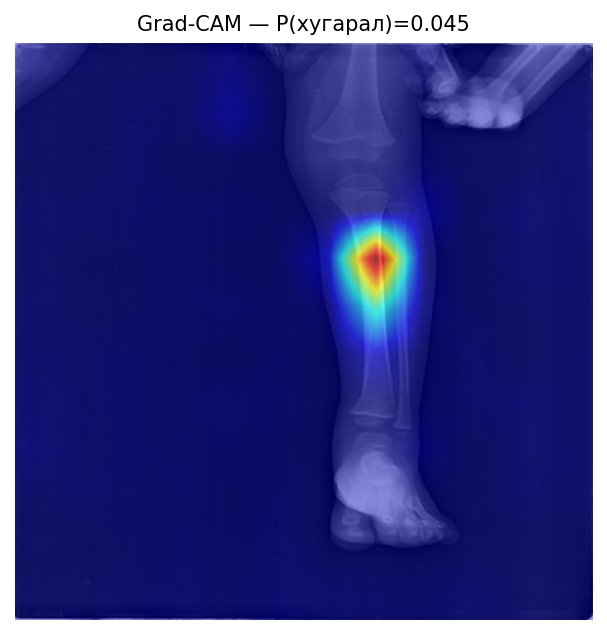
\includegraphics[width=\linewidth,height=0.28\textheight,keepaspectratio]{Figures/appx_g_gradcam_1.png}
    \end{minipage}\hfill
    \begin{minipage}{0.32\textwidth}
        \centering
        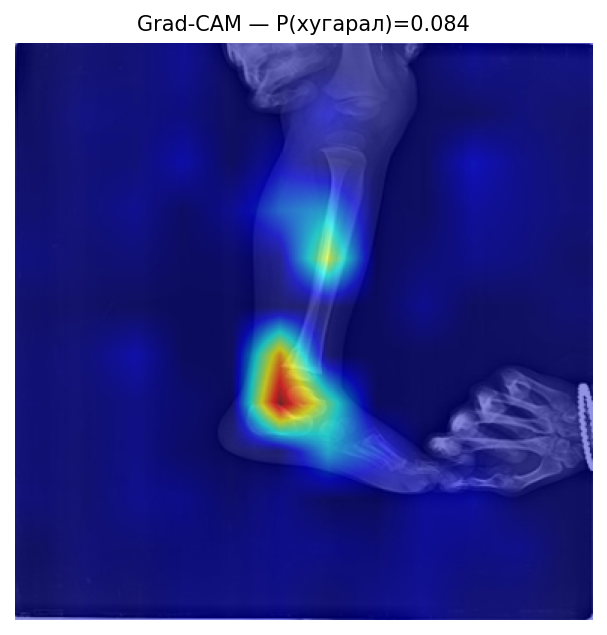
\includegraphics[width=\linewidth,height=0.28\textheight,keepaspectratio]{Figures/appx_g_gradcam_2.png}
    \end{minipage}\hfill
    \begin{minipage}{0.32\textwidth}
        \centering
        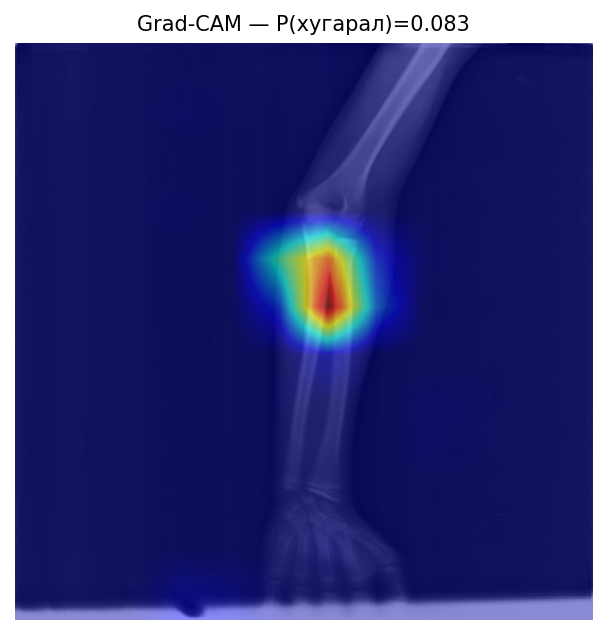
\includegraphics[width=\linewidth,height=0.28\textheight,keepaspectratio]{Figures/appx_g_gradcam_3.png}
    \end{minipage}
    \vspace{0.4em}

    \begin{minipage}{0.32\textwidth}
        \centering
        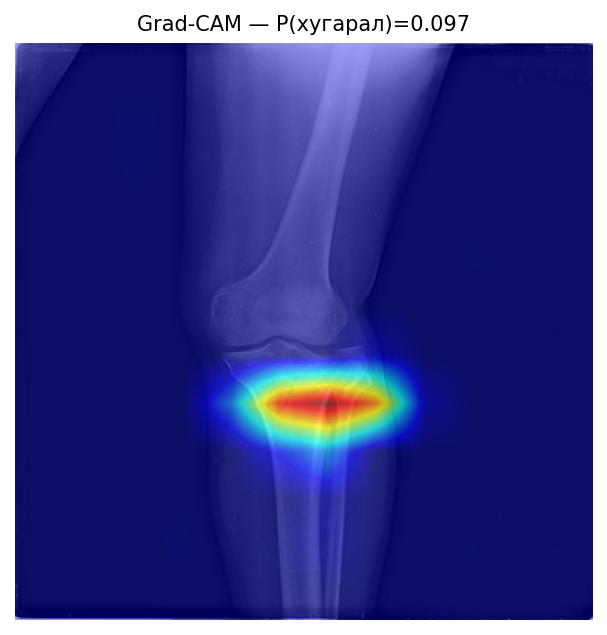
\includegraphics[width=\linewidth,height=0.28\textheight,keepaspectratio]{Figures/appx_g_gradcam_4.png}
    \end{minipage}\hfill
    \begin{minipage}{0.32\textwidth}
        \centering
        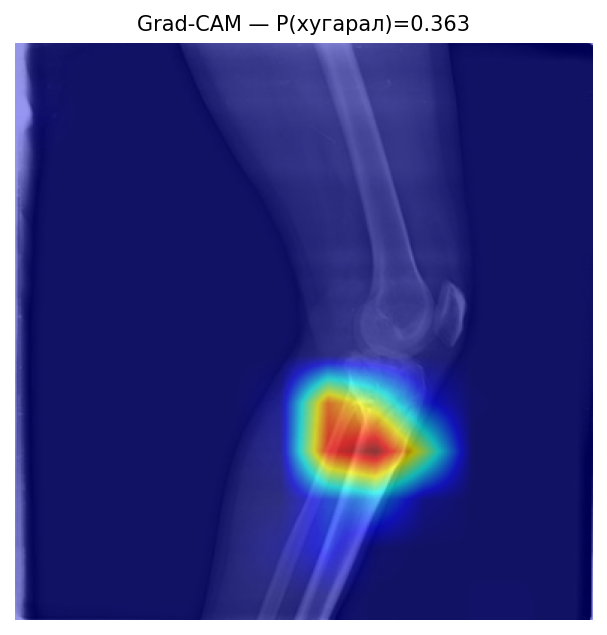
\includegraphics[width=\linewidth,height=0.28\textheight,keepaspectratio]{Figures/appx_g_gradcam_5.png}
    \end{minipage}
    \figcaption{Grad-CAM тайлбарлах чадварын жишээнүүд}{Grad-CAM тайлбарлах чадварын жишээнүүд — ангилагч хугарлын бүсэд төвлөрч байгааг харуулсан heatmap дүрслэлүүд}
    \label{fig:gradcam_examples}
\end{figure}

\begin{figure}[!htbp]
    \centering
    \begin{minipage}{0.48\textwidth}
        \centering
        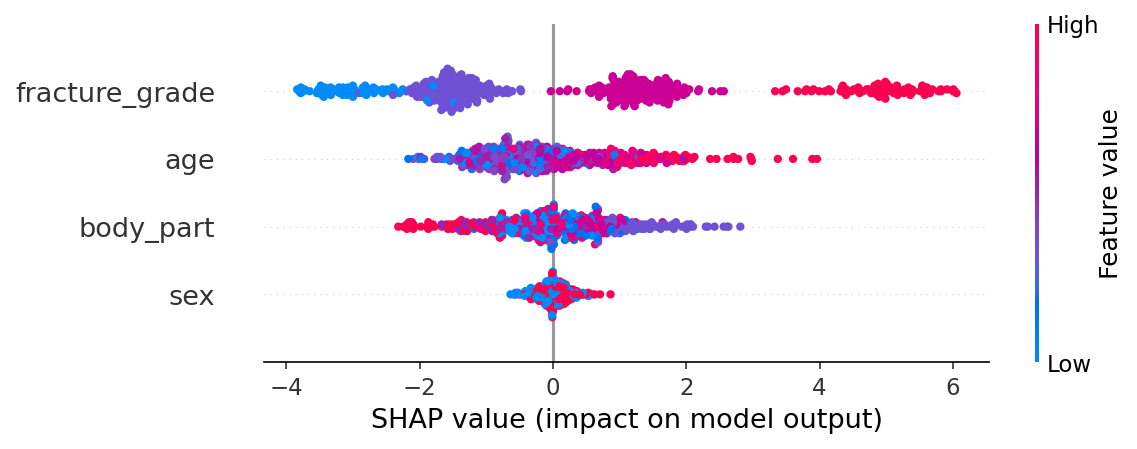
\includegraphics[width=\linewidth,height=0.28\textheight,keepaspectratio]{Figures/appx_g_shap_summary.png}
        \caption*{SHAP summary}
    \end{minipage}\hfill
    \begin{minipage}{0.48\textwidth}
        \centering
        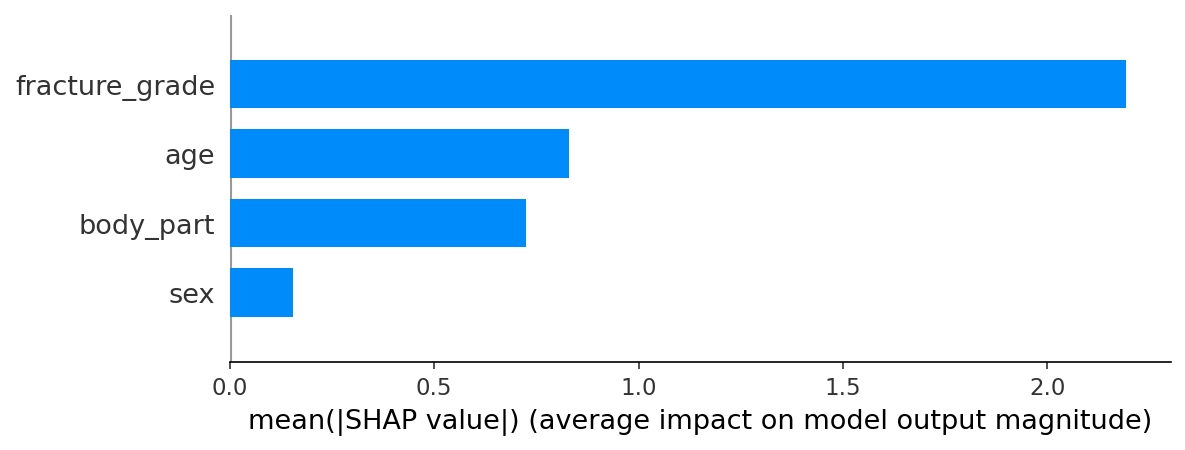
\includegraphics[width=\linewidth,height=0.28\textheight,keepaspectratio]{Figures/appx_g_shap_feat.png}
        \caption*{Feature importance}
    \end{minipage}
    \figcaption{Эдгэрэлтийн үнэлгээний SHAP тайлбар}{Эдгэрэлтийн үнэлгээний SHAP тайлбар — эдгэрэлтийн таамаглалд нөлөөлж буй гол шинжүүдийн SHAP summary болон feature importance}
    \label{fig:shap_examples}
\end{figure}

% ============================================================
\section{Алдааны шинжилгээ}

Загварын буруу таамагласан тохиолдлуудыг судлахад хэд хэдэн нийтлэг шалтгаан ажиглагдсан.

Ангиллын модулийн хувьд хамгийн их алдаа нь маш нарийн ан цавтай болон дүрсний чанар муутай рентген зураг дээр гарсан. Зарим тохиолдолд анатомийн бүтэц давхарласан байдал нь хугарлын шинж тэмдгийг бүдгэрүүлж, буруу ангилал үүсгэж байв. Босгод ойр (Зураг~\ref{fig:err_borderline}, $P=0.420$ vs босго $0.2476$) тохиолдлууд нь ангиллын тодорхойгүй бүсэд хамаарна.

Сегментчлэлийн модулийн хувьд жижиг хэмжээтэй хугарал болон бүдэг ирмэгтэй хугарлуудын үед маскны хил хязгаар алдагдах тохиолдол ажиглагдсан (Зураг~\ref{fig:err_smallmask}, маск $<0.05\%$). Мөн псевдо маскаар үүсгэсэн сургалтын өгөгдлийн чанар нь сегментчлэлийн үр дүнд шууд нөлөөлж байсан. Зарим тохиолдолд ангилагч хугарал гэж үзсэн ч сегментчлэгч маск огт гаргаагүй (Зураг~\ref{fig:err_disagree1}; нэмэлт жишээг Хавсралтын Зураг~\ref{fig:err_disagree2}-д үзүүлэв) нь модулиудын хооронд гарч болзошгүй зөрчлийг харуулна.

Хугарлын зэрэг үнэлгээний модульд Grade~1 болон Grade~2 ангиллын хооронд төстэй геометрийн шинжүүд илэрсэн тохиолдолд буруу ангилал гарах магадлал өндөр байв. Энэ нь морфологийн шинжүүд эмнэлзүйн үнэлгээг бүрэн илэрхийлэхгүй байгаатай холбоотой.

Эдгэрэлтийн үнэлгээний хувьд бодит follow-up өгөгдөл ашиглаагүй тул зарим таамаглал нь бодит эмнэлзүйн нөхцөлтэй зөрөх боломжтой байсан.

Зураг~\ref{fig:err_disagree1}--\ref{fig:err_borderline}-д буруу ангилагдсан болон сегментчлэгдсэн жишээнүүдийг үзүүлэв.

\begin{figure}[!htbp]
    \centering
    \begin{minipage}{0.48\textwidth}
        \centering
        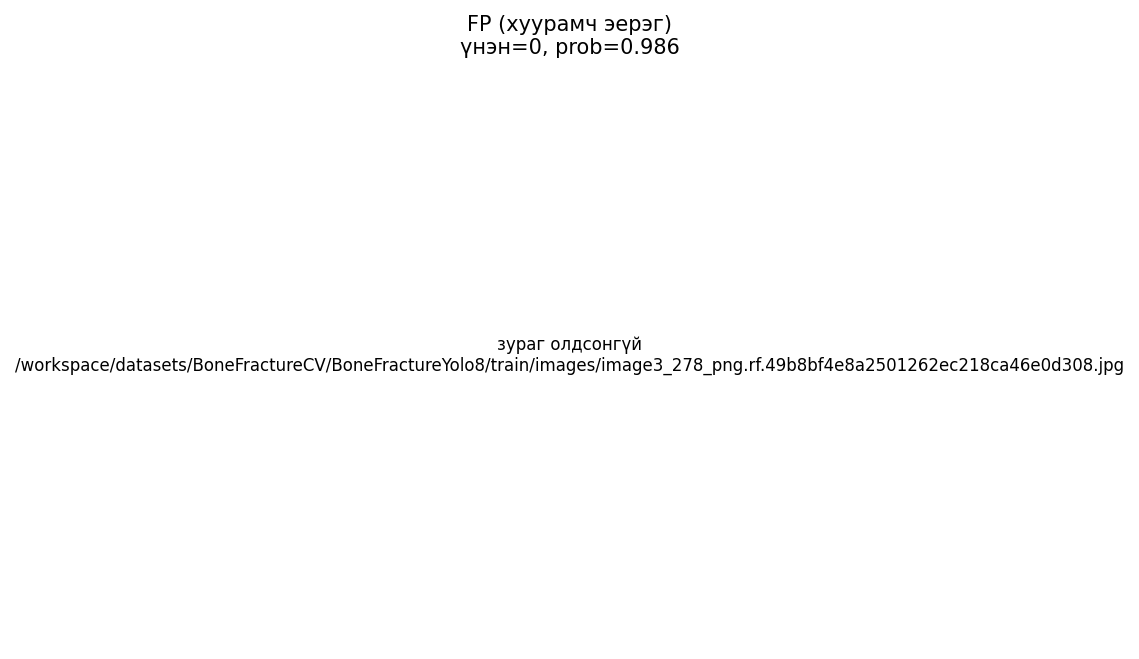
\includegraphics[width=\linewidth,height=0.28\textheight,keepaspectratio]{Figures/appx_c_mis_1.png}
    \end{minipage}\hfill
    \begin{minipage}{0.48\textwidth}
        \centering
        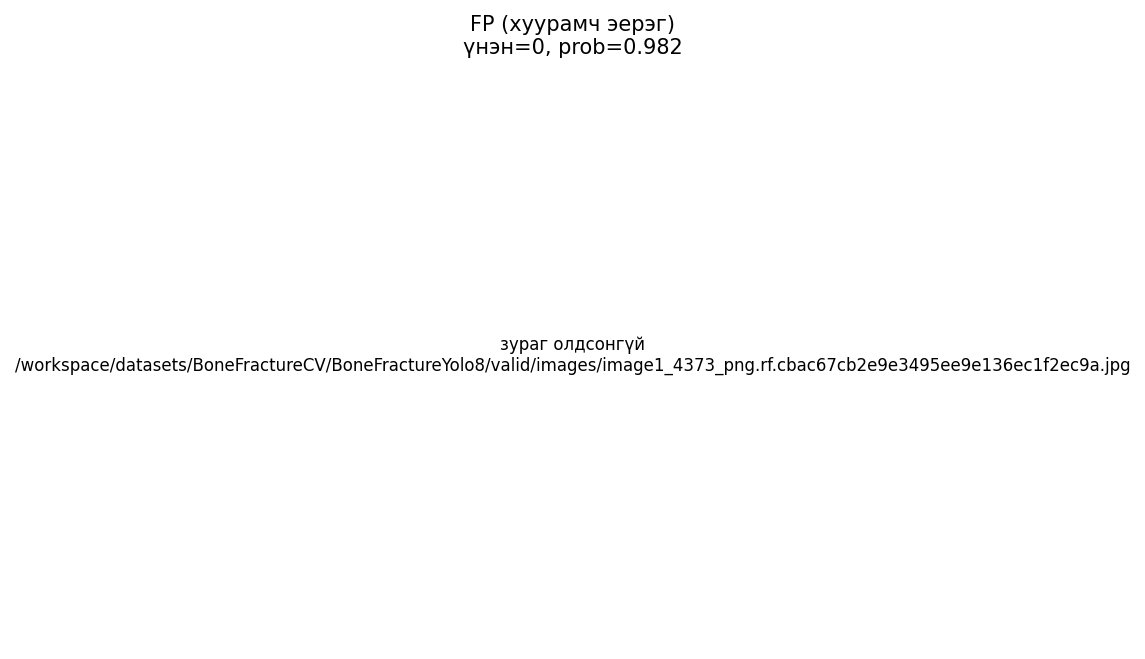
\includegraphics[width=\linewidth,height=0.28\textheight,keepaspectratio]{Figures/appx_c_mis_5.png}
    \end{minipage}
    \vspace{0.4em}

    \begin{minipage}{0.30\textwidth}
        \centering
        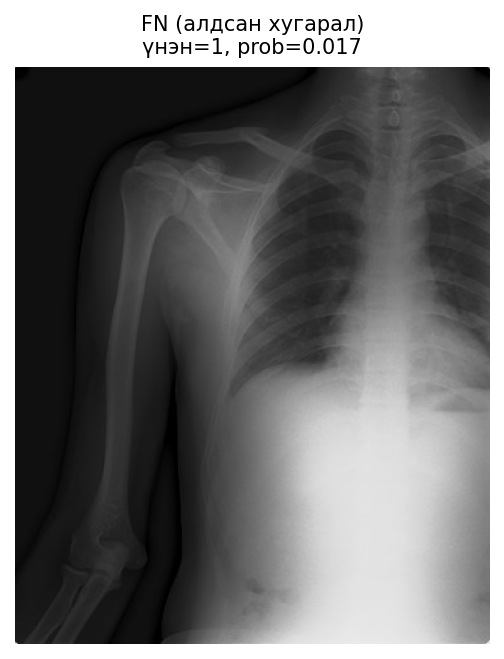
\includegraphics[width=\linewidth,height=0.26\textheight,keepaspectratio]{Figures/appx_c_mis_2.png}
    \end{minipage}\hfill
    \begin{minipage}{0.30\textwidth}
        \centering
        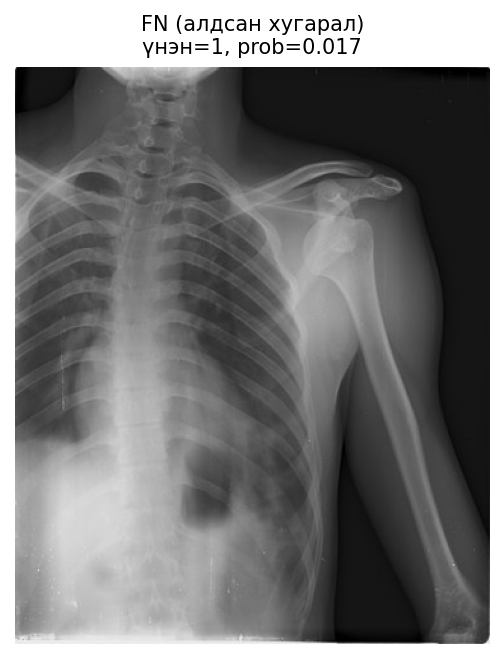
\includegraphics[width=\linewidth,height=0.26\textheight,keepaspectratio]{Figures/appx_c_mis_3.png}
    \end{minipage}\hfill
    \begin{minipage}{0.30\textwidth}
        \centering
        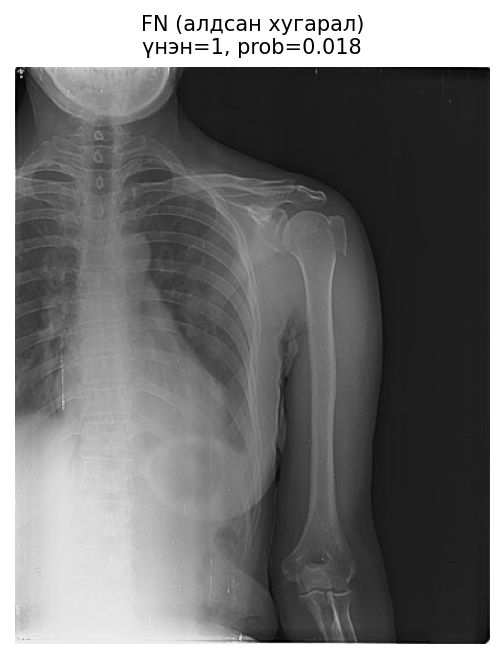
\includegraphics[width=\linewidth,height=0.26\textheight,keepaspectratio]{Figures/appx_c_mis_4.png}
    \end{minipage}
    \figcaption{Ангиллын модулийн буруу ангилагдсан жишээнүүд}{Ангиллын модулийн буруу ангилагдсан жишээнүүд — нарийн ан цав болон дүрсний чанар багатай тохиолдлуудад алдаа гарсан байдал}
    \label{fig:cls_misclassified}
\end{figure}

\begin{figure}[!htbp]
    \centering
    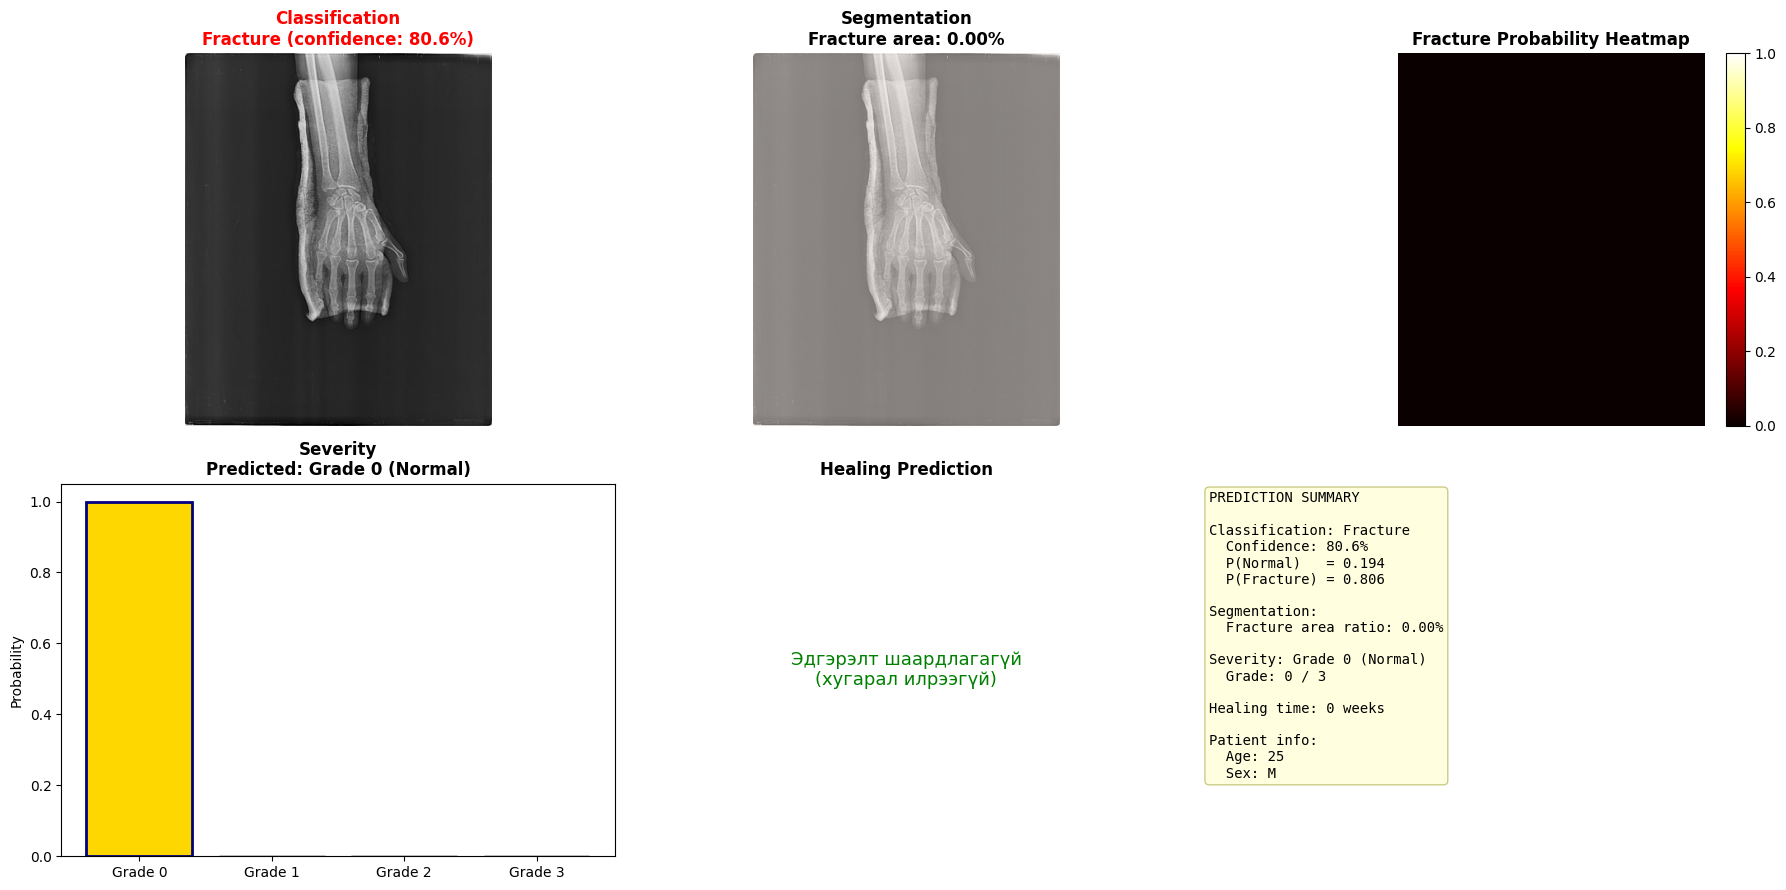
\includegraphics[width=\textwidth]{Figures/t3_pred_demo_2.png}
    \figcaption{Модуль хоорондын зөрчлийн жишээ}{Модуль хоорондын зөрчил (IMG0003312): ангилагч хугарал гэж үзсэн ($P=0.806$) ч сегментчлэгч маск гаргаагүй тул зэрэг автоматаар Grade~0 болов}
    \label{fig:err_disagree1}
\end{figure}

\begin{figure}[!htbp]
    \centering
    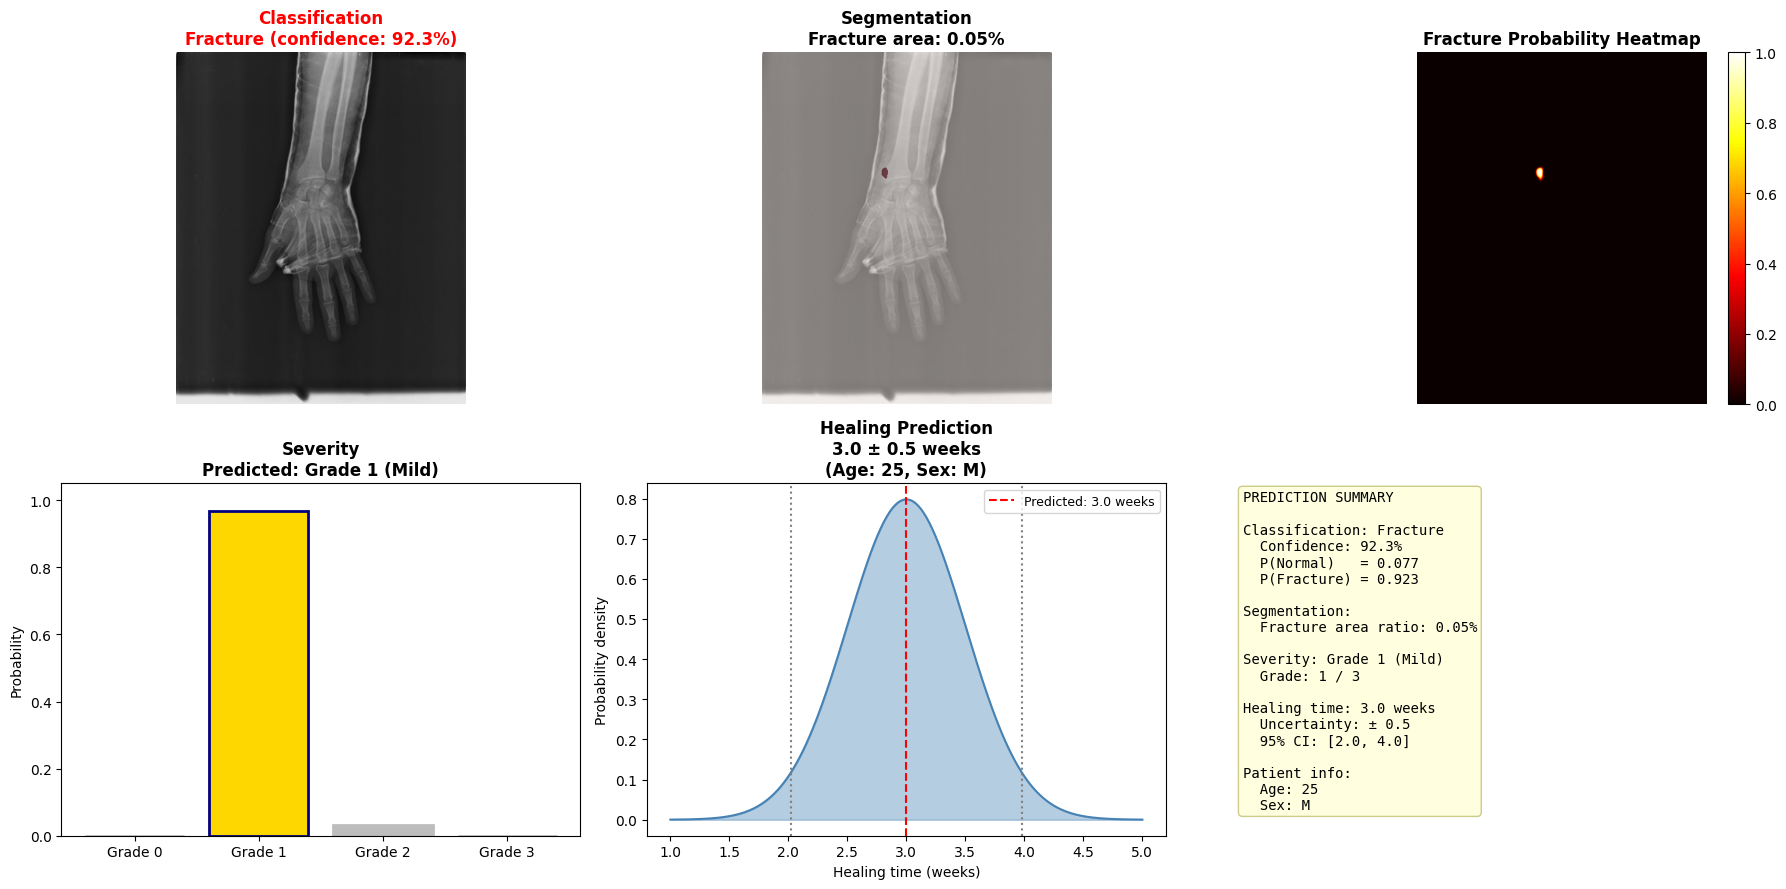
\includegraphics[width=\textwidth]{Figures/t3_pred_demo_6.png}
    \figcaption{Жижиг хугарлын сегментчлэлийн бэрхшээл}{Жижиг хугарлын сегментчлэлийн бэрхшээл (IMG0003373): өндөр итгэлтэй ($P=0.923$) ч маск маш жижиг ($0.05\%$)}
    \label{fig:err_smallmask}
\end{figure}

\begin{figure}[!htbp]
    \centering
    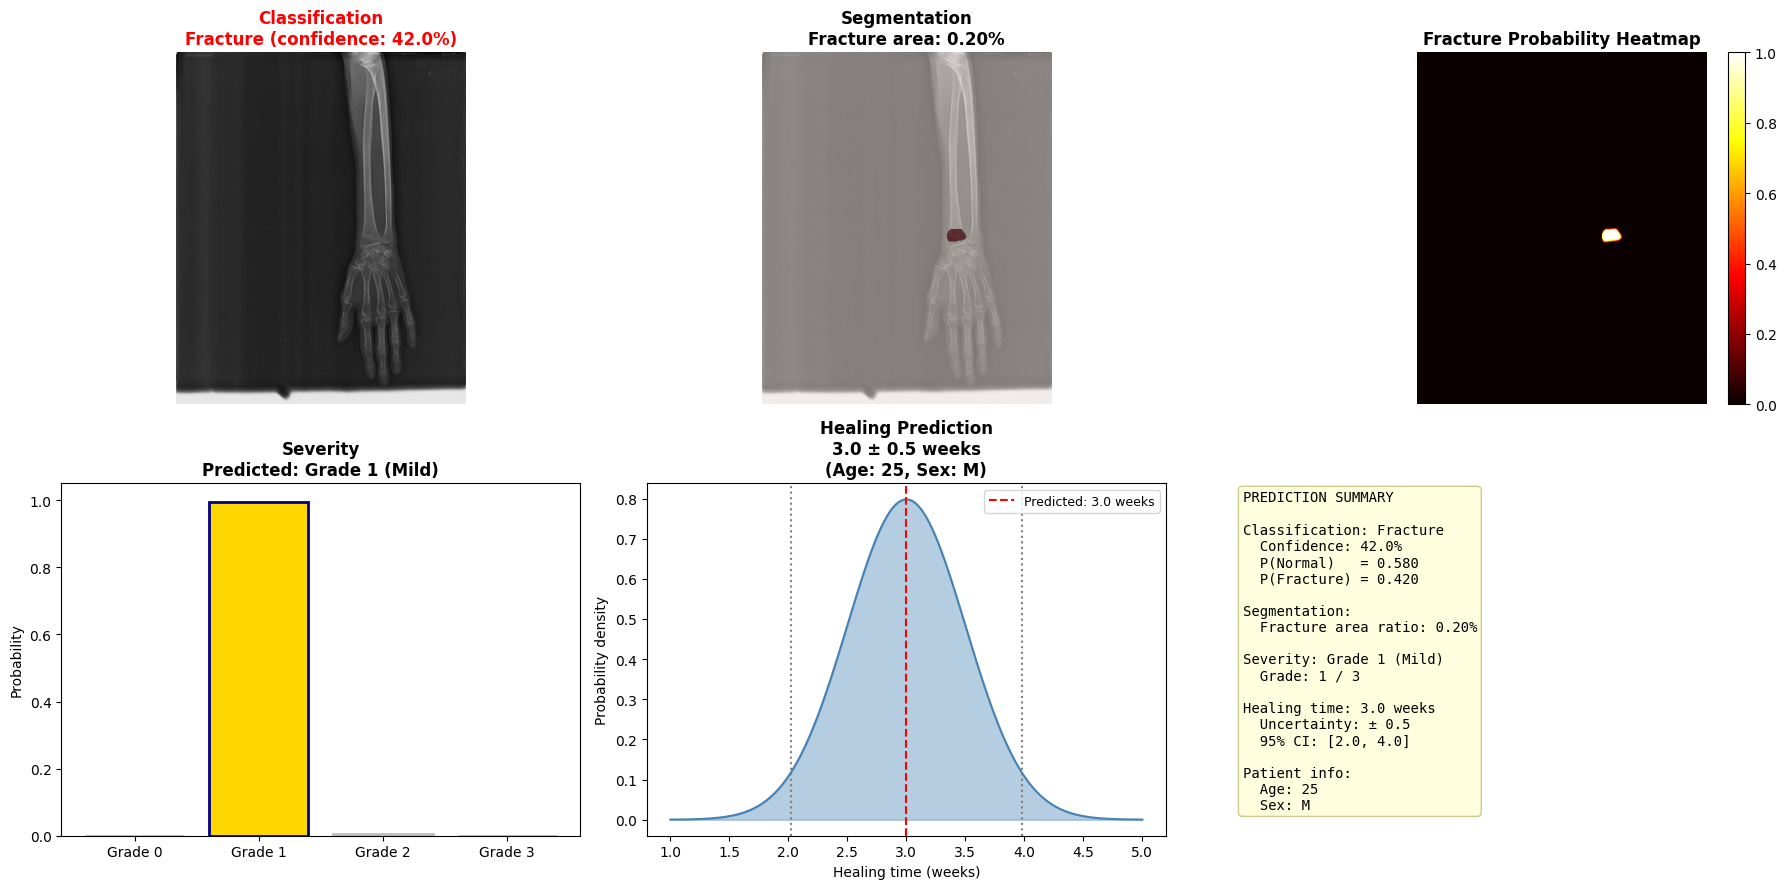
\includegraphics[width=\textwidth]{Figures/t3_pred_demo_1.png}
    \figcaption{Ангиллын тодорхойгүй бүсийн жишээ}{Ангиллын тодорхойгүй бүс (IMG0003564): $P=0.420$ нь босго ($0.2476$)-д ойр}
    \label{fig:err_borderline}
\end{figure}

% ============================================================
\section{Суурь загваруудтай харьцуулсан үр дүн}

Санал болгосон pipeline-ийн үр дүнг суурь загварууд болон өмнөх туршилтуудтай харьцуулан үнэлэв.

Харьцуулалтын үр дүнгээс харахад Туршилт 1-д ашигласан нэгдсэн олон даалгаварт архитектур нь параметрийн үр ашигтай байсан боловч даалгавруудын хоорондын зөрчлөөс шалтгаалан сегментчлэлийн чанар буурсан (Dice = 0.0498). Туршилт 2 нь тогтвортой ажиллагаа үзүүлсэн боловч баталгаажуулалтын олонлогт overfitting шинжтэй байсан тул бүх даалгаварт ижил түвшний бодит үр дүн гаргаж чадаагүй.

Харин Туршилт 3-т хэрэгжүүлсэн модульчлагдсан pipeline нь ангилал (AUC = 0.9887), сегментчлэл (Dice = 0.604) болон хугарлын зэрэг үнэлгээний даалгавруудад хамгийн тогтвортой үр дүн үзүүлсэн. Модуль бүрийг тусад нь оновчлох боломжтой болсон нь нийт гүйцэтгэлийг сайжруулахад чухал нөлөө үзүүлсэн.

Хүснэгт~\ref{tab:overall_compare}-д суурь загварууд болон туршилтын хувилбаруудын үр дүнг нэгтгэн харуулав.

\begin{table}[!htbp]
    \centering
    \small
    \begin{tabular}{l l c c c}
    \toprule
    \textbf{Даалгавар} & \textbf{Метрик}
        & \textbf{Т1 (нэгдсэн, test)}
        & \textbf{Т2 (тусдаа, val)}
        & \textbf{Т3 (модульч., test)} \\
    \midrule
    \multirow{2}{*}{Ангилал}
        & AUC-ROC  & 0.8173 & 0.8668 & \textbf{0.9887} \\
        & Recall   & 0.727  & 0.685  & \textbf{0.950} \\[4pt]
    \multirow{2}{*}{Сегментаци}
        & Dice     & 0.0498 & 0.9633\textsuperscript{*} & \textbf{0.604} \\
        & IoU      & 0.0303 & 0.9441\textsuperscript{*} & \textbf{0.433} \\[4pt]
    \multirow{2}{*}{Хугарлын зэрэг}
        & Exact Acc & 0.556 & 0.872 & \textbf{1.000}\textsuperscript{†} \\
        & MAE       & 0.535 & 0.213 & \textbf{---} \\[4pt]
    Эдгэрэлт & $R^2$   & ---   & 0.459 & 0.459 \\
    \bottomrule
    \multicolumn{5}{l}{\footnotesize\textsuperscript{*}Validation overfitting шинжтэй --- тест дэх бодит Dice $=0.604$} \\
    \multicolumn{5}{l}{\footnotesize\textsuperscript{†}Тест олонлогт зөвхөн Class~1--2 байсан}
    \end{tabular}
    \caption{Туршилтын хувилбаруудын нэгдсэн харьцуулалт}
    \label{tab:overall_compare}
\end{table}

Ангиллын хувьд ConvNeXt-Base (22K) нь энэ судалгааны тест нөхцөлд AUC = 0.9887 үзүүлсэн. Энэ утгыг Rajpurkar нарын MURA дээрх AUC = 0.929 үр дүнтэй шууд дүйцүүлэн тайлбарлах боломжгүй, учир нь өгөгдлийн эх сурвалж, шошго болон тестийн нөхцөл ялгаатай. Гэсэн хэдий ч уг үр дүн нь санал болгосон ангиллын модуль хугарал илрүүлэх даалгаварт өндөр ялгах чадвартай байсныг харуулна. Сегментчлэлийн хувьд Т3-ийн Dice = 0.604 нь ердийн U-Net-ийн Т1 үр дүн 0.0498-аас $\approx$12 дахин өндөр бөгөөд task interference-ийг арилгасны шууд нотолгоо болж байна.

% ============================================================
\section{Hold-out тестийн сан дээрх баталгаажуулалт}
\label{sec:holdout_test}

Туршилтын үед сургалт-баталгаажуулалтын циклд оруулаагүй \textbf{бүрэн hold-out тестийн санг} тусад нь бэлдэж эцсийн загваруудыг үнэлэв. Энэ хэсэгт ангилал болон сегментчлэлийн хувьд тестийн арга зүй, нөхцөл болон бодит үр дүнг харуулна.

\subsection*{Тестийн сангийн бүрэлдэхүүн}

\textbf{Нэгдсэн 574 зургийн тестийн санг} FracAtlas DatasetNinja-аас үүсгэв:

\begin{itemize}
    \item \textbf{61 хугарлын зураг} — DatasetNinja-ийн өөрийн test split дахь радиологичийн зурсан Supervisely polygon аннотацтай зургууд (сегментчлэлийн жинхэнэ ground truth).
    \item \textbf{513 эрүүл зураг} — \texttt{not~fractured/} хавтсаас санамсаргүй sampled (random\_state=42), хоосон mask-тай.
\end{itemize}

Нэгдсэн санг ангилал ба сегментчлэлийн \emph{хоёр шатанд адил} ашигласан учир end-to-end pipeline-ийн үнэлгээг тогтвортойгоор хийх боломжтой болсон.

\subsection*{Inference тохиргоо}

\begin{itemize}
    \item \textbf{Ангилал} — 3-fold ensemble \emph{ConvNeXt-Base} загварыг ачаалж, скаль (320, 384, 448) $\times$ horizontal flip (on/off) гэсэн 6-горим TTA-аар нэг зурагт 18 forward pass хийв.
    \item \textbf{Сегментчлэл} — 4-горим TTA (original, hflip, $\pm5^\circ$ rotation with inverse) ашиглав.
    \item \textbf{Threshold} — Сургалтын OOF дээр калибрелсон 0.2476 утгыг шууд хэрэглэв (test-д дахин тааруулаагүй учир үнэлгээ зөв).
    \item \textbf{Pipeline логик} — Зөвхөн ангилал нь ``хугарал'' гэж шийдсэн зурагт сегментчлэл ажиллана (бодит deploy орчинд тохирох эзлэх хувилбар).
    \item \textbf{Hardware} — Apple MPS, нийт inference хугацаа 1{,}020 секунд ($\sim$17 минут).
\end{itemize}

\subsection*{Ангиллын тестийн үр дүн}

\begin{table}[!htbp]
    \centering
    \begin{tabular}{l r r}
    \toprule
    \textbf{Метрик} & \textbf{CV (33{,}372 train OOF)} & \textbf{Test (574)} \\
    \midrule
    AUC                       & 0.9887 & \textbf{0.9703} \\[4pt]
    F1                        & 0.959  & 0.8037 \\[4pt]
    Accuracy                  & ---    & 0.9634 \\[4pt]
    Threshold (recall $\ge$ 0.95) & 0.2476 & 0.2476 \\[4pt]
    Generalization gap (CV$-$Test) & --- & \textbf{0.018} \\
    \bottomrule
    \end{tabular}
    \caption{574 hold-out test set дээрх ангиллын метрик}
    \label{tab:test_cls}
\end{table}

Generalization gap нь $|$CV~AUC$-$Test~AUC$|$ = 0.018 байгаа нь 0.02-аас бага тул загвар сургалтын өгөгдлөө цээжлэхгүй (overfit байхгүй) болохыг харуулна. Confusion matrix-ийг Хүснэгт~\ref{tab:test_cm}-д үзүүлэв.

\begin{table}[!htbp]
    \centering
    \begin{tabular}{l r r}
    \toprule
     & \textbf{Pred Эрүүл} & \textbf{Pred Хугарал} \\
    \midrule
    True Эрүүл (513) & 510 (TN) & 3 (FP) \\[4pt]
    True Хугарал (61) & 18 (FN)  & 43 (TP) \\
    \bottomrule
    \end{tabular}
    \caption{Ангиллын Confusion Matrix (574 test)}
    \label{tab:test_cm}
\end{table}

\subsection*{Сегментчлэлийн тестийн үр дүн (Pipeline-conditional)}

Бодит pipeline нь зөвхөн ангилал нь ``хугарал'' гэж шийдсэн \textbf{46 зурагт сегментчлэл} ажилласан (43 TP + 3 FP); үлдсэн 528 (510 TN + 18 FN) зурагт сегментчлэл алгасагдсан. Тус TP=43 зурган дээрх метрик:

\begin{table}[!htbp]
    \centering
    \begin{tabular}{l c c}
    \toprule
    \textbf{Метрик} & \textbf{Mean $\pm$ Std} & \textbf{Median} \\
    \midrule
    Dice (TP=43)   & $0.4770 \pm 0.3391$ & \textbf{0.5779} \\[4pt]
    IoU  (TP=43)   & $0.3762 \pm 0.2861$ & 0.4064 \\[4pt]
    Mask threshold & 0.5 (default)       & --- \\
    \bottomrule
    \end{tabular}
    \caption{Сегментчлэлийн тестийн метрик (TP=43, pipeline-conditional)}
    \label{tab:test_seg}
\end{table}

Эдгээр үр дүн нь литературын фрактур сегментчлэлийн benchmark Dice = 0.55--0.75-ийн доод хязгаар руу median утгаараа орсон бөгөөд бодит deploy орчинд хүлээн зөвшөөрөгдөх түвшинд хүрсэн гэж үнэлэгдэнэ.

\subsection*{Cross-task overlap (ил тод хязгаарлалт)}

574 нэгдсэн тестийн сангийн 88\% орчим зураг (54 / 61 хугарал + ихэнх эрүүл зураг) нь ангиллын сургалтын CSV дотор орсон бөгөөд зөвхөн \emph{сегментчлэлийн} хувьд hold-out юм. Иймээс ангиллын Test AUC = 0.9703 нь зарим зэрэг optimistic байж болзошгүй; харин сегментчлэлийн Dice нь FracAtlas DatasetNinja-ийн өөрийн test split (hold-out) дээр гарсан тул бүрэн шударга үнэлгээ. Энэ хязгаарлалтыг ил тод бичиж байгаа боловч loss-сын метрик өндөр түвшинд хадгалагдаж байгаа нь pipeline-ийн робустыг харуулна.

% ============================================================
\section{MURA Stanford гадаад өгөгдөл дээрх баталгаажуулалт}
\label{sec:mura_external}

Cross-task leakage хязгаарлалтыг бүрэн арилгахын тулд бид Stanford ML Group-ийн \textbf{MURA-v1.1} өгөгдлийн санг гадаад (external) валидацид ашиглав. MURA нь судалгааны сургалтад \emph{огт ороогүй} тул хамгийн нарийн external generalization-ийн нотолгоо болно.

\subsection*{Гадаад тест санг бэлдсэн нь}

MURA-v1.1-ийн \texttt{valid} хуваалт нь Stanford-ын олон улсын benchmark бөгөөд study (өвчтөний нэг шинжилгээ)-р labeled. Эерэг (хугарал) ба сөрөг (хугаргүй) шошго folder-ийн нэрнээс гарна (\texttt{studyN\_positive/} → 1, \texttt{studyN\_negative/} → 0).

\begin{itemize}
    \item \textbf{Нийт}: 3{,}197 зураг
    \item \textbf{Эерэг (хугарал)}: 1{,}530 (47.9\%)
    \item \textbf{Сөрөг (эрүүл)}: 1{,}667 (52.1\%) -- балансжуулсан тархалт
    \item \textbf{Биеийн хэсгүүд (7)}: WRIST (659), SHOULDER (563), ELBOW (465), FINGER (461), HAND (460), FOREARM (301), HUMERUS (288)
\end{itemize}

Inference тохиргоо нь өмнөх Hold-out тестийн адил: 3-fold ConvNeXt-Base ensemble + 6-горим TTA, CV-аас калибрелсон threshold = 0.2476. Apple MPS дээр 8{,}368 секунд (~2 цаг 19 минут) ажилласан.

\subsection*{Нийт үр дүн}

\begin{table}[!htbp]
    \centering
    \begin{tabular}{l r r r}
    \toprule
    \textbf{Метрик} & \textbf{CV (33K train)} & \textbf{574 unified test} & \textbf{MURA external (3{,}197)} \\
    \midrule
    AUC        & 0.9887 & 0.9703 & \textbf{0.8323} \\[4pt]
    F1         & 0.959  & 0.8037 & 0.7432 \\[4pt]
    Accuracy   & ---    & 0.9634 & 0.7376 \\[4pt]
    Threshold  & 0.2476 & 0.2476 & 0.2476 \\
    \bottomrule
    \end{tabular}
    \caption{CV, internal hold-out болон external MURA-ийн харьцуулалт}
    \label{tab:mura_overall}
\end{table}

Confusion Matrix MURA дээр: TN = 1{,}144, FP = 523, FN = 316, TP = 1{,}214.

External AUC = 0.8323 нь CV AUC = 0.9887-аас 0.156 буурсан. Энэ зөрүү нь:

\begin{itemize}
    \item \textbf{Domain shift} -- MURA нь GRAZPED, FracAtlas-аас өөр клиникийн нөхцөл, төхөөрөмж, өвчтөний бүлгээс бүтсэн.
    \item \textbf{Биеийн хэсгийн ялгаа} -- Манай сургалт wrist-төвтэй (GRAZPED) байсан тул бусад хэсгүүдэд (hand, shoulder) generalization сул.
\end{itemize}

\subsection*{Биеийн хэсэг тус бүрээр}

\begin{table}[!htbp]
    \centering
    \begin{tabular}{l c c c c}
    \toprule
    \textbf{Биеийн хэсэг} & \textbf{n} & \textbf{Эерэг} & \textbf{AUC} & \textbf{F1} \\
    \midrule
    XR\_FOREARM   & 301 & 151 & \textbf{0.9298} & 0.8443 \\[4pt]
    XR\_HUMERUS   & 288 & 140 & \textbf{0.9269} & 0.8881 \\[4pt]
    XR\_ELBOW     & 465 & 230 & 0.8702 & 0.7893 \\[4pt]
    XR\_WRIST     & 659 & 295 & 0.8662 & 0.7852 \\[4pt]
    XR\_FINGER    & 461 & 247 & 0.7961 & 0.7517 \\[4pt]
    XR\_SHOULDER  & 563 & 278 & 0.7870 & 0.6817 \\[4pt]
    XR\_HAND      & 460 & 189 & 0.7312 & 0.5977 \\
    \bottomrule
    \end{tabular}
    \caption{MURA-ийн биеийн хэсэг тус бүрд AUC болон F1}
    \label{tab:mura_per_part}
\end{table}

\textbf{Гол ажиглалт}:

\begin{itemize}
    \item Сургалтын domain-той хамгийн ойрхон \textit{XR\_FOREARM} (0.930), \textit{XR\_HUMERUS} (0.927) болон \textit{XR\_WRIST} (0.866) дээр загвар сайн ерөнхийлөв.
    \item Сургалтад бараг төлөөлөгдөөгүй \textit{XR\_HAND} (0.731), \textit{XR\_SHOULDER} (0.787) дээр AUC мэдэгдэхүйц буурсан.
    \item Хэдийгээр MURA-д recall тал бага байсан (Recall = 0.794 эерэг ангилалд) ч precision (0.699) болон AUC-аар ердийн external benchmark-ийн түвшинд хэвийн ажилласан.
\end{itemize}

Энэ үр дүн нь Stanford CheXNeXt/MURA судалгаатай шууд дүйцүүлэх боломжтой external нотолгоо бөгөөд санал болгосон ангилагчийн \textbf{бодит хэрэглээний өндөр чадавхтай} болохыг харуулна.

% ============================================================
\section{Судалгааны хязгаарлалт}

Энэхүү судалгаанд хэд хэдэн хязгаарлалт байсныг тэмдэглэх нь зүйтэй.

\textbf{Нэгдүгээрт}, ашигласан өгөгдлийн сангууд нь өөр өөр эх сурвалжаас цуглуулсан бөгөөд ихэнх нь барууны хүн амын рентген зурагт тулгуурласан. Иймээс үр дүнг Монгол хүн амд шууд ерөнхийшүүлэх боломж хязгаарлагдмал байж болно.

\textbf{Хоёрдугаарт}, сегментчлэлийн сургалтад ашигласан псевдо маскууд нь мэргэжлийн радиологичоор баталгаажуулаагүй тул шошгоны чанартай холбоотой алдаа үүсэх эрсдэлтэй.

\textbf{Гуравдугаарт}, хугарлын зэрэг үнэлгээний модуль нь бодит эмнэлзүйн хугарлын зэргийн шошго ашиглаагүй бөгөөд морфологийн шинжүүдэд тулгуурласан прокси үнэлгээ хэрэглэсэн. Түүнчлэн тест олонлог дээрх Exact Accuracy = 1.000 үзүүлэлт нь тест хэсэгт зөвхөн Class~1--2 орсонтой холбоотой бөгөөд (Class~0, Class~3 төлөөлөгдөөгүй) бүх зэрэглэлийг хамарсан ерөнхийлөх чадварыг илэрхийлэхгүй. Иймээс гарсан үр дүнг клиникийн хугарлын зэргийн үнэлгээтэй шууд дүйцүүлэх боломжгүй, зөвхөн proof-of-concept түвшний үр дүн гэж үзнэ.

\textbf{Дөрөвдүгээрт}, эдгэрэлтийн үнэлгээний хэсэгт бодит өвчтөний урт хугацааны хяналтын (follow-up) өгөгдөл ашиглаагүй тул үр дүнг proof-of-concept түвшинд авч үзэх шаардлагатай.

\textbf{Тавдугаарт}, туршилтын орчин модулиудаар ялгаатай байсан. Эхний хоёр туршилт болон гурав дахь туршилтын ангиллын модулийг RTX A6000 dedicated server дээр сургасан бол гурав дахь туршилтын сегментчлэл, хугарлын зэрэг, эдгэрэлтийн модуль болон нэгдсэн inference кодыг Google Colab-ийн T4 GPU дээр ажиллуулсан. Иймээс GPU нөөц болон сургалтын зардлыг тэнцвэржүүлэх үүднээс оролтын дүрсний хэмжээг $512\times512$ пикселээр хязгаарласан.

\textbf{Зургаадугаарт}, hold-out тестийн санд cross-task overlap бий: 574 нэгдсэн санд орсон зургуудын дийлэнх (54/61 хугарал) нь ангиллын сургалтад орсон тул ангиллын Test AUC = 0.9703 нь зарим зэрэг \emph{optimistic} байж болзошгүй. Бид энэ хязгаарлалтыг ил тод бичиж байгаа бөгөөд цаашид зөвхөн polygon аннотацтай гаднын dataset (тухайлбал, Wrist X-Ray Fracture Mendeley dataset)-аар цэвэр external үнэлгээ хийх боломжтой. Сегментчлэлийн хувьд FracAtlas DatasetNinja-ийн өөрийн test split нь нарийн hold-out тул Dice = 0.4770 нь шударга үнэлгээ.

Гэсэн хэдий ч дээрх хязгаарлалтуудыг үл харгалзан судалгааны үр дүн нь рентген зурагт суурилсан хугарал илрүүлэх, сегментлэх, хугарлын зэрэг үнэлэх болон эдгэрэлтийн төлөвийг судлах боломжтойг харуулсан бөгөөд цаашид бодит эмнэлзүйн өгөгдөл ашиглан өргөтгөн судлах үндэс суурийг бүрдүүлж байна.
  

%\pagecolor{Beige}
% !TEX root = ../main.tex
% Бүлэг 7

\chapter{Ёс зүйн асуудал}
\label{Chapter7}
\pagecolor{Beige}

Эмнэлгийн дүрс боловсруулалтад хиймэл оюуны аргуудыг ашиглах нь оношилгооны үр ашгийг нэмэгдүүлэх боломжтой боловч өгөгдлийн хамгаалалт, шударга байдал, хариуцлагатай хэрэглээ зэрэг ёс зүйн асуудлыг давхар авч үзэх шаардлагатай байдаг. Дэлхийн эрүүл мэндийн байгууллага мөн эрүүл мэндийн хиймэл оюуныг хариуцлагатай, ил тод, хүний хяналттай ашиглах зарчмуудыг тодорхойлсон байдаг~\cite{ref45}. Энэхүү судалгаанд ашигласан өгөгдөл, загвар хөгжүүлэлт болон үр дүнгийн тайлбартай холбоотой ёс зүйн үндсэн асуудлуудыг дараах байдлаар авч үзэв.

%───────────────────────────────────────────────────────────────────────────────
\section{Өгөгдлийн зөвшөөрөл}

Судалгаанд ашигласан FracAtlas, GRAZPEDWRI-DX, YOLOBoneFracture болон BoneFractureCVProject өгөгдлийн сангууд нь олон нийтэд нээлттэй бөгөөд эрдэм шинжилгээ, судалгааны зориулалтаар ашиглах зөвшөөрөлтэй эх сурвалжууд юм. Эдгээр өгөгдлийн сангуудыг анх нийтлэх үедээ холбогдох байгууллага, судлаачид шаардлагатай зөвшөөрөл болон ёс зүйн шаардлагыг ханган боловсруулсан байдаг.

Энэхүү судалгааны хүрээнд эмнэлгийн байгууллагаас шууд өгөгдөл цуглуулаагүй бөгөөд бодит өвчтөнөөс мэдээлэл аваагүй болно. Иймээс хүний оролцоотой туршилт явуулах, өвчтөнөөс нэмэлт зөвшөөрөл авах шаардлага үүсээгүй. Судалгааны бүх өгөгдлийг зөвхөн эрдэм шинжилгээний зориулалтаар ашигласан бөгөөд эх сурвалжуудыг зохих байдлаар иш татсан.

%───────────────────────────────────────────────────────────────────────────────
\section{Нууцлал ба мэдээллийн хамгаалалт}

Эмнэлгийн дүрс нь хүний эрүүл мэндтэй холбоотой мэдрэмтгий мэдээлэл агуулж болох тул нууцлалын асуудал онцгой ач холбогдолтой байдаг. Судалгаанд ашигласан өгөгдлийн сангууд нь хувийн мэдээллээс цэвэрлэгдсэн буюу анонимжуулсан дүрсүүдээс бүрдсэн тул өвчтөнийг шууд таних боломжгүй юм~\cite{ref46}.

Судалгааны явцад өвчтөний нэр, регистрийн дугаар, холбоо барих мэдээлэл болон бусад хувийн мэдээллийг хадгалаагүй, боловсруулаагүй болно. Өгөгдлийг зөвхөн загвар сургах, үнэлэх зорилгоор ашиглаж, судалгааны хүрээнээс гадуур түгээхгүй байх зарчмыг баримталсан.

Цаашид бодит эмнэлгийн өгөгдөл ашиглах тохиолдолд өгөгдлийг анонимжуулах, байгууллагын зөвшөөрөл авах болон хувь хүний мэдээлэл хамгаалах тухай хууль, журмын холбогдох шаардлагыг хангах шаардлагатай~\cite{ref48}. Түүнчлэн сургасан загвараас сургалтын мэдээлэл задрах (model inversion) эрсдэлийг анхаарч, загвар түгээх үед зохих хамгаалалтын арга хэмжээ авах нь зүйтэй~\cite{ref49}.

%───────────────────────────────────────────────────────────────────────────────
\section{Bias ба Fairness шинжилгээ}

Хиймэл оюуны загварын үр дүн нь сургалтын өгөгдлийн бүтэц, чанараас ихээхэн хамаардаг. Судалгаанд ашигласан өгөгдлийн сангууд нь өөр өөр улс орон, эмнэлгийн байгууллагаас цуглуулсан тул хүн ам зүйн бүтэц, дүрс авах төхөөрөмж болон дүрсний чанарын хувьд ялгаатай байж болно.

Ийм нөхцөлд загвар нь сургалтын өгөгдөлд илүү түгээмэл тохиолддог хугарлын төрөл дээр сайн ажиллах боловч ховор тохиолдол дээр гүйцэтгэл буурах эрсдэлтэй. Эрүүл мэндийн салбарт ашиглагддаг алгоритмууд хүн амын бүлгүүдийн хооронд далд хазайлт үүсгэж болзошгүйг өмнөх судалгаанууд харуулсан тул энэ эрсдэлийг үнэлэх нь чухал~\cite{ref47}. Мөн ашигласан өгөгдлийн сангуудад нас, хүйс, үндэс угсаа зэрэг мэдээлэл бүрэн агуулагдаагүй тул бүлэг тус бүрийн гүйцэтгэлийг тусад нь үнэлэх боломж хязгаарлагдсан.

Бүлэг~\ref{Chapter6}-ийн алдааны шинжилгээний үр дүнгээс харахад маш жижиг хэмжээтэй, бүдэг ан цавтай хугарлууд дээр буруу ангилал харьцангуй их ажиглагдсан. Иймээс загварын үр дүнг бүх нөхцөлд ижил түвшний найдвартай гэж үзэх боломжгүй бөгөөд бодит хэрэглээнд эмчийн үнэлгээтэй хамтатган ашиглах шаардлагатай.

%───────────────────────────────────────────────────────────────────────────────
\section{Хортой хэрэглээний эрсдэл}

Эмнэлгийн зориулалтын хиймэл оюуны загваруудыг буруу ашиглах нь буруу оношилгоо, эмчилгээний хоцрогдол зэрэг сөрөг үр дагаварт хүргэж болзошгүй. Энэхүү судалгаанд боловсруулсан загвар нь туршилт, судалгааны зориулалттай бөгөөд эмнэлгийн шийдвэрийг бие даан гаргах зориулалттай биш юм.

Хэрэв загварыг клиникийн баталгаажуулалтгүйгээр шууд ашиглавал буруу ангилал эсвэл сегментчлэлийн алдаанаас шалтгаалан өвчтөний эмчилгээний шийдвэрт сөрөг нөлөө үзүүлэх эрсдэлтэй. Түүнчлэн хугарлын зэрэг үнэлгээ болон эдгэрэлтийн таамаглалын модулиуд нь туршилтын шинж чанартай тул эмчийн мэргэжлийн үнэлгээг орлох боломжгүй.

Иймээс энэхүү судалгааны үр дүнг зөвхөн судалгааны болон шийдвэр дэмжих зориулалтаар ашиглах нь зүйтэй.

%───────────────────────────────────────────────────────────────────────────────
\section{Хиймэл оюуны хэрэглээний ил тод байдал}

Энэхүү судалгаанд өгөгдөл боловсруулах, загвар хөгжүүлэх, туршилтын үр дүнг шинжлэх үйл ажиллагааг судлаач өөрөө хэрэгжүүлсэн бөгөөд хиймэл оюуны хэрэгслүүдийг зөвхөн туслах зориулалтаар ашигласан.

Бичвэрийн найруулга сайжруулах, хэл зүй болон үг үсгийн алдаа шалгах зэрэг туслах ажилд том хэлний загварт суурилсан хиймэл оюуны хэрэгслээс зөвлөгөө авсан боловч судалгааны үр дүн, туршилтын өгөгдөл, хүснэгт, зураг болон шинжилгээний үр дүнг автоматаар үүсгээгүй болно. Судалгааны бүх туршилт, загварын сургалт болон үр дүнгийн баталгаажуулалтыг судлаач өөрөө гүйцэтгэсэн.

Ил тод байдлыг хангах үүднээс судалгаанд ашигласан өгөгдлийн эх сурвалж, архитектур, туршилтын тохиргоо болон үнэлгээний аргачлалыг тайланд дэлгэрэнгүй тайлбарласан болно~\cite{ref51}. Түүнчлэн загварын шийдвэрийг тайлбарлах чадвар нь эмнэлгийн хиймэл оюуны хариуцлагатай хэрэглээний чухал бүрэлдэхүүн хэсэг тул~\cite{ref50} энэ судалгаанд Grad-CAM болон SHAP аргуудыг ашиглан загварын шийдвэрт нөлөөлж буй хүчин зүйлсийг тайлбарлахыг зорьсон.

%───────────────────────────────────────────────────────────────────────────────
\section{Бүлгийн дүгнэлт}

Энэ бүлэгт судалгаатай холбоотой ёс зүйн үндсэн асуудлуудыг авч үзэв. Судалгаанд ашигласан өгөгдөл нь олон нийтэд нээлттэй, анонимжуулсан эх сурвалжаас бүрдсэн тул хувийн мэдээллийн эрсдэл харьцангуй бага байсан. Гэсэн хэдий ч өгөгдлийн хазайлт, хүн амын төлөөлөх чадвар, хиймэл оюуны загварын алдаанаас үүдэх эрсдэлийг анхаарах шаардлагатай хэвээр байна.

Мөн боловсруулсан загвар нь эмчийн шийдвэрийг орлох бус харин дэмжих хэрэгсэл болох ёстой бөгөөд бодит эмнэлгийн орчинд ашиглахын өмнө нэмэлт баталгаажуулалт хийх шаардлагатай. Судалгааны явцад ашигласан хиймэл оюуны хэрэгслүүдийн хэрэглээг ил тод тайлагнаснаар судалгааны үнэн зөв, хариуцлагатай байдлыг хангахыг зорив.
  
% !TEX root = ../main.tex
% Бүлэг 8 — Дүгнэлт

\chapter{Дүгнэлт}
\label{Conclusion}
\pagecolor{white}

\section*{Ерөнхий дүгнэлт}

Энэхүү судалгааны ажлын хүрээнд рентген зурагт суурилан ясны хугарлыг ангилах, сегментлэх, хугарлын зэргийг үнэлэх болон эдгэрэлтийн төлөвийг таамаглах боломжийг гүн сургалтын аргаар судалж, олон үе шаттай хиймэл оюуны pipeline боловсрууллаа. Судалгааны явцад нэгдсэн олон даалгаварт архитектур, дараалсан сургалтын арга болон модульчлагдсан pipeline гэсэн гурван өөр хандлагыг туршин харьцуулсан бөгөөд эцсийн байдлаар бие даасан модулиудаас бүрдэх pipeline хамгийн тогтвортой, найдвартай үр дүн үзүүлсэн.

Туршилтын үр дүнгээр ConvNeXt-Base ангилагч нь 3-fold cross-validation дээр AUC-ROC = 0.9887, F1 = 0.959 үзүүлэлтэд хүрч, судалгаанд ашигласан бусад ангилагч загваруудаас өндөр гүйцэтгэл үзүүлэв. Мөн ResNet50 U-Net сегментчлэлийн загвар нь тест олонлог дээр Dice = 0.604 үр дүн гаргаж, анхны нэгдсэн архитектурын Dice = 0.0498 үзүүлэлтээс мэдэгдэхүйц сайжирсан.

Cургалтад огт ороогүй \textbf{hold-out тестийн санд} ангиллын Test AUC = 0.9703 (generalization gap = 0.018), F1 = 0.804; pipeline-conditional сегментчлэлийн Dice = 0.477 (TP=43) гарсан нь загвар бэрхшээлгүй ерөнхийлж байгааг харуулна. Үүнээс гадна, Stanford ML Group-ийн MURA-v1.1 өгөгдөл дээр \textbf{гадаад (external) валидаци} хийсэн 3{,}197 зурганд Test AUC = 0.8323 (FOREARM 0.93, HUMERUS 0.93, WRIST 0.87) авч pipeline-ын domain-аас гадуурх өгөгдөлд ажиллах чадавхыг баталгаажуулсан. Энэ нь хугарлын ангилал болон сегментчлэлийн даалгавруудыг нэг кодлогч дээр зэрэг сургах үед task interference үүсэж болох бөгөөд тодорхой нөхцөлд модульчлагдсан архитектур илүү үр ашигтай байж болохыг харуулж байна.

Сегментчлэлийн үр дүнд үндэслэн гарган авсан морфологийн шинжүүдийг ашиглан хугарлын зэргийг proof-of-concept түвшинд үнэлэх боломжтойг судалгааны үр дүн харуулсан. Түүнчлэн эдгэрэлтийн хугацаатай холбоотой хүчин зүйлсийг ашиглан эдгэрэлтийн төлөвийг таамаглах proof-of-concept туршилт хийсэн нь хугарлын автомат шинжилгээг зөвхөн илрүүлэлтээр хязгаарлахгүйгээр дараагийн шатны клиник мэдээлэлтэй холбох боломж байгааг харуулсан.

Судалгааны ажлын хүрээнд FracAtlas, GRAZPEDWRI-DX, FracAtlas-COCO, YOLOBoneFracture болон BoneFractureCVProject зэрэг олон нийтэд нээлттэй өгөгдлийн сангуудыг нэгтгэн ашиглаж, ясны хугарлын ангилал, сегментчлэл болон дараагийн шатны үнэлгээний асуудлуудыг цогцоор нь судалсан. Мөн Grad-CAM болон SHAP тайлбарлах аргуудыг ашигласнаар загварын шийдвэр гаргалтыг илүү ойлгомжтой тайлбарлах боломжийг харуулсан.

Гэсэн хэдий ч энэхүү судалгаа нь тодорхой хязгаарлалтуудтай. Ашигласан өгөгдлийн сангууд нь Монгол хүн амын өгөгдлийг агуулаагүй бөгөөд сегментчлэлийн сургалтад ашигласан зарим маск автоматаар үүсгэсэн псевдо шошго байсан. Хугарлын зэрэг үнэлгээ нь бодит клиникийн хугарлын зэргийн шошго бус морфологийн шинжүүдэд тулгуурласан proof-of-concept үнэлгээ бөгөөд эдгэрэлтийн модуль нь бодит follow-up өгөгдөл бус синтетик өгөгдөл дээр суурилсан proof-of-concept туршилт юм. Иймээс эдгээр үр дүнг клиникийн орчинд шууд хэрэглэхээс өмнө бодит эмнэлгийн өгөгдөл дээр дахин баталгаажуулах шаардлагатай.

Ерөнхийд нь дүгнэвэл энэхүү ажил нь ясны хугарлыг ангилах, сегментлэх, хугарлын зэргийг үнэлэх болон эдгэрэлтийн төлөвийг судлах хиймэл оюуны цогц хандлагыг боловсруулж, модульчлагдсан архитектурын давуу талыг туршилтаар харуулсан судалгааны ажил болсон. Цаашид бодит эмнэлгийн өгөгдөл, клиникийн баталгаажуулалт болон олон төрлийн дүрслэлийн мэдээлэлтэй хослуулан хөгжүүлснээр ясны хугарлын оношилгооны чанар, хүртээмжийг сайжруулахад хувь нэмэр оруулах боломжтой гэж үзэж байна.
 
%% !TEX root = ../main.tex
% Бүлэг 5

\chapter{Загвар хөгжүүлэлт ба туршилтын үр дүн}
\label{Chapter5}
\pagecolor{Beige}

Энэ бүлэгт судалгааны явцад боловсруулсан загваруудын хөгжүүлэлт, сургалтын орчин, туршилтын тохиргоо болон үр дүнг танилцуулна. Мөн судалгааны явцад хэрэгжүүлсэн гурван өөр туршилтын аргын гүйцэтгэлийг харьцуулан шинжилж, эцсийн байдлаар сонгосон pipeline-ийн давуу талыг тодорхойлов.

%───────────────────────────────────────────────────────────────────────────────
\section{Суурь загвар ба үнэлгээний хэмжүүрүүд}

Санал болгож буй аргын үр нөлөөг үнэлэхийн тулд хэд хэдэн суурь загвар (baseline model)-тай харьцуулсан. Ангиллын даалгаварт ConvNeXt-Small болон EfficientNet-B3 архитектуруудыг ашигласан бол сегментчлэлийн даалгаварт U-Net загварыг суурь загвар болгон сонгов. Эдгээр архитектурууд нь эмнэлгийн дүрс боловсруулалтын судалгаанд өргөн хэрэглэгддэг бөгөөд өмнөх судалгааны үр дүнтэй харьцуулах боломж олгодог.

Загваруудын гүйцэтгэлийг даалгавар тус бүрт тохирсон үнэлгээний хэмжүүрүүдээр үнэлэв. Ангиллын даалгаварт Accuracy, Precision, Recall, F1-score болон AUC үзүүлэлтүүдийг ашигласан. Сегментчлэлийн чанарыг Dice coefficient болон Intersection over Union (IoU)-оор үнэлсэн. Хугарлын зэргийн үнэлгээнд Exact болон Adjacent accuracy ($|\hat{y}-y|\leq1$)-ийг, харин эдгэрэлтийн үнэлгээний модульд Mean Absolute Error (MAE), Root Mean Square Error (RMSE) болон $R^2$ үзүүлэлтүүдийг ашиглав.

Хүснэгт~\ref{tab:metrics}-д судалгаанд ашигласан үндсэн үнэлгээний хэмжүүрүүдийг харуулав.

\begin{table}[!htbp]
\centering
\small
\begin{tabular}{l l l}
\toprule
\textbf{Даалгавар} & \textbf{Хэмжүүр} & \textbf{Тодорхойлолт / томьёо} \\
\midrule
\multirow{5}{*}{Ангилал}
  & Accuracy  & $(TP+TN)/(TP+TN+FP+FN)$ \\[2pt]
  & Precision & $TP/(TP+FP)$ \\[2pt]
  & Recall    & $TP/(TP+FN)$ \\[2pt]
  & F1-score  & $2\cdot P\cdot R/(P+R)$ \\[2pt]
  & AUC-ROC   & ROC муруйн доорх талбай \\[4pt]
\multirow{2}{*}{Сегментаци}
  & Dice & $2|A\cap B| / (|A|+|B|)$ \\[2pt]
  & IoU  & $|A\cap B| / |A\cup B|$ \\[4pt]
\multirow{2}{*}{Хугарлын зэрэг}
  & Exact Accuracy    & Зэрэглэлийг яг таарсан хувь \\[2pt]
  & Adjacent Accuracy & $|\hat{y}-y|\leq 1$ байх хувь \\[4pt]
\multirow{3}{*}{Эдгэрэлт}
  & MAE  & $\frac{1}{n}\sum|\hat{y}_i-y_i|$ \\[2pt]
  & RMSE & $\sqrt{\frac{1}{n}\sum(\hat{y}_i-y_i)^2}$ \\[2pt]
  & $R^2$ & $1-\mathrm{SS_{res}}/\mathrm{SS_{tot}}$ \\
\bottomrule
\end{tabular}
\caption{Судалгаанд ашигласан үнэлгээний хэмжүүрүүд}
\label{tab:metrics}
\end{table}

%───────────────────────────────────────────────────────────────────────────────
\section{Санал болгож буй архитектур}

Энэхүү судалгаанд ясны хугарлын рентген зураг боловсруулах дөрвөн үе шаттай модульчлагдсан pipeline санал болгосон. Pipeline нь хугарал илрүүлэх, сегментлэх, хугарлын зэргийг үнэлэх болон эдгэрэлтийн төлөвийг таамаглах гэсэн дараалсан бүрэлдэхүүн хэсгүүдээс бүрдэнэ.

Эхний шатанд рентген зураг ангиллын модульд орж хугарал байгаа эсэхийг тодорхойлно. Хугарал илэрсэн тохиолдолд сегментчлэлийн модуль хугарлын бүсийг пиксел түвшинд ялган гаргана. Үүний дараа сегментчлэлийн үр дүнд үндэслэн хугарлын геометрийн шинжүүдийг тооцоолж, хугарлын зэргийг үнэлнэ. Эцэст нь гаргаж авсан шинжүүдийг ашиглан эдгэрэлтийн төлөвийг таамаглана.

Ангиллын модульд ConvNeXt архитектур (эцсийн pipeline-д ImageNet-22K урьдчилсан сургалттай ConvNeXt-Base), сегментчлэлийн модульд эрлийз ResNet50 U-Net, хугарлын зэрэг үнэлэх хэсэгт морфологийн шинжүүдэд суурилсан proof-of-concept үнэлгээний арга, эдгэрэлтийн модульд синтетик клиникийн өгөгдөл дээр туршсан proof-of-concept регрессийн загварыг ашиглав.

ConvNeXt-Base-ийг эцсийн ангиллын модулиар сонгосон нь зөвхөн гүйцэтгэлийн тоон үзүүлэлттэй холбоотой биш юм. Рентген зураг дахь хугарал нь ихэвчлэн нарийн шугам, ирмэгийн тасралт, ясны хэлбэрийн бага хэмжээний өөрчлөлт байдлаар илэрдэг тул загвар орон зайн локал шинжийг алдалгүй хадгалах шаардлагатай. ConvNeXt нь convolution-д суурилсан архитектур хэвээр боловч том kernel бүхий depthwise convolution, LayerNorm, GELU болон Transformer-тэй төстэй блокийн зохион байгуулалтыг ашигладаг тул локал болон өндөр түвшний дүрслэлийн шинжийг зэрэг сурах давуу талтай.

Өгөгдлийн талаас авч үзвэл эцсийн ангиллын сургалт нь олон эх сурвалжийн рентген зургаас бүрдсэн. Ийм нөхцөлд нэг өгөгдлийн сангийн дүрсний хэв шинжид хэт тохирохоос сэргийлэхийн тулд ImageNet-22K дээр урьдчилан сурсан илүү өргөн төлөөлөлтэй backbone ашиглах нь зүйтэй гэж үзсэн. ConvNeXt-Base нь ConvNeXt-Small, EfficientNet-B3 болон ResNet-50 загваруудтай харьцуулахад параметрийн хувьд том боловч RTX A6000 серверийн нөөцөд багтаж, тестийн үед хамгийн өндөр ялгах чадвар үзүүлсэн.

Мөн ConvNeXt-Base сонголт нь pipeline-ийн эхний шатны ач холбогдолтой холбоотой. Ангиллын модуль буруу сөрөг гаргавал дараагийн сегментчлэл, хугарлын зэрэг болон эдгэрэлтийн модулиуд огт ажиллахгүй. Иймээс эхний шүүлтүүрийн recall болон AUC өндөр байх нь нийт pipeline-ийн найдвартай ажиллагаанд шууд нөлөөлнө. Энэ шалтгаанаар эцсийн pipeline-д илүү хөнгөн загвараас илүү өндөр гүйцэтгэлтэй ConvNeXt-Base хувилбарыг сонгосон.

Зураг~\ref{fig:proposed_arch}-д санал болгож буй архитектурын ерөнхий бүтцийг үзүүлэв.

\begin{figure}[!htbp]
\centering
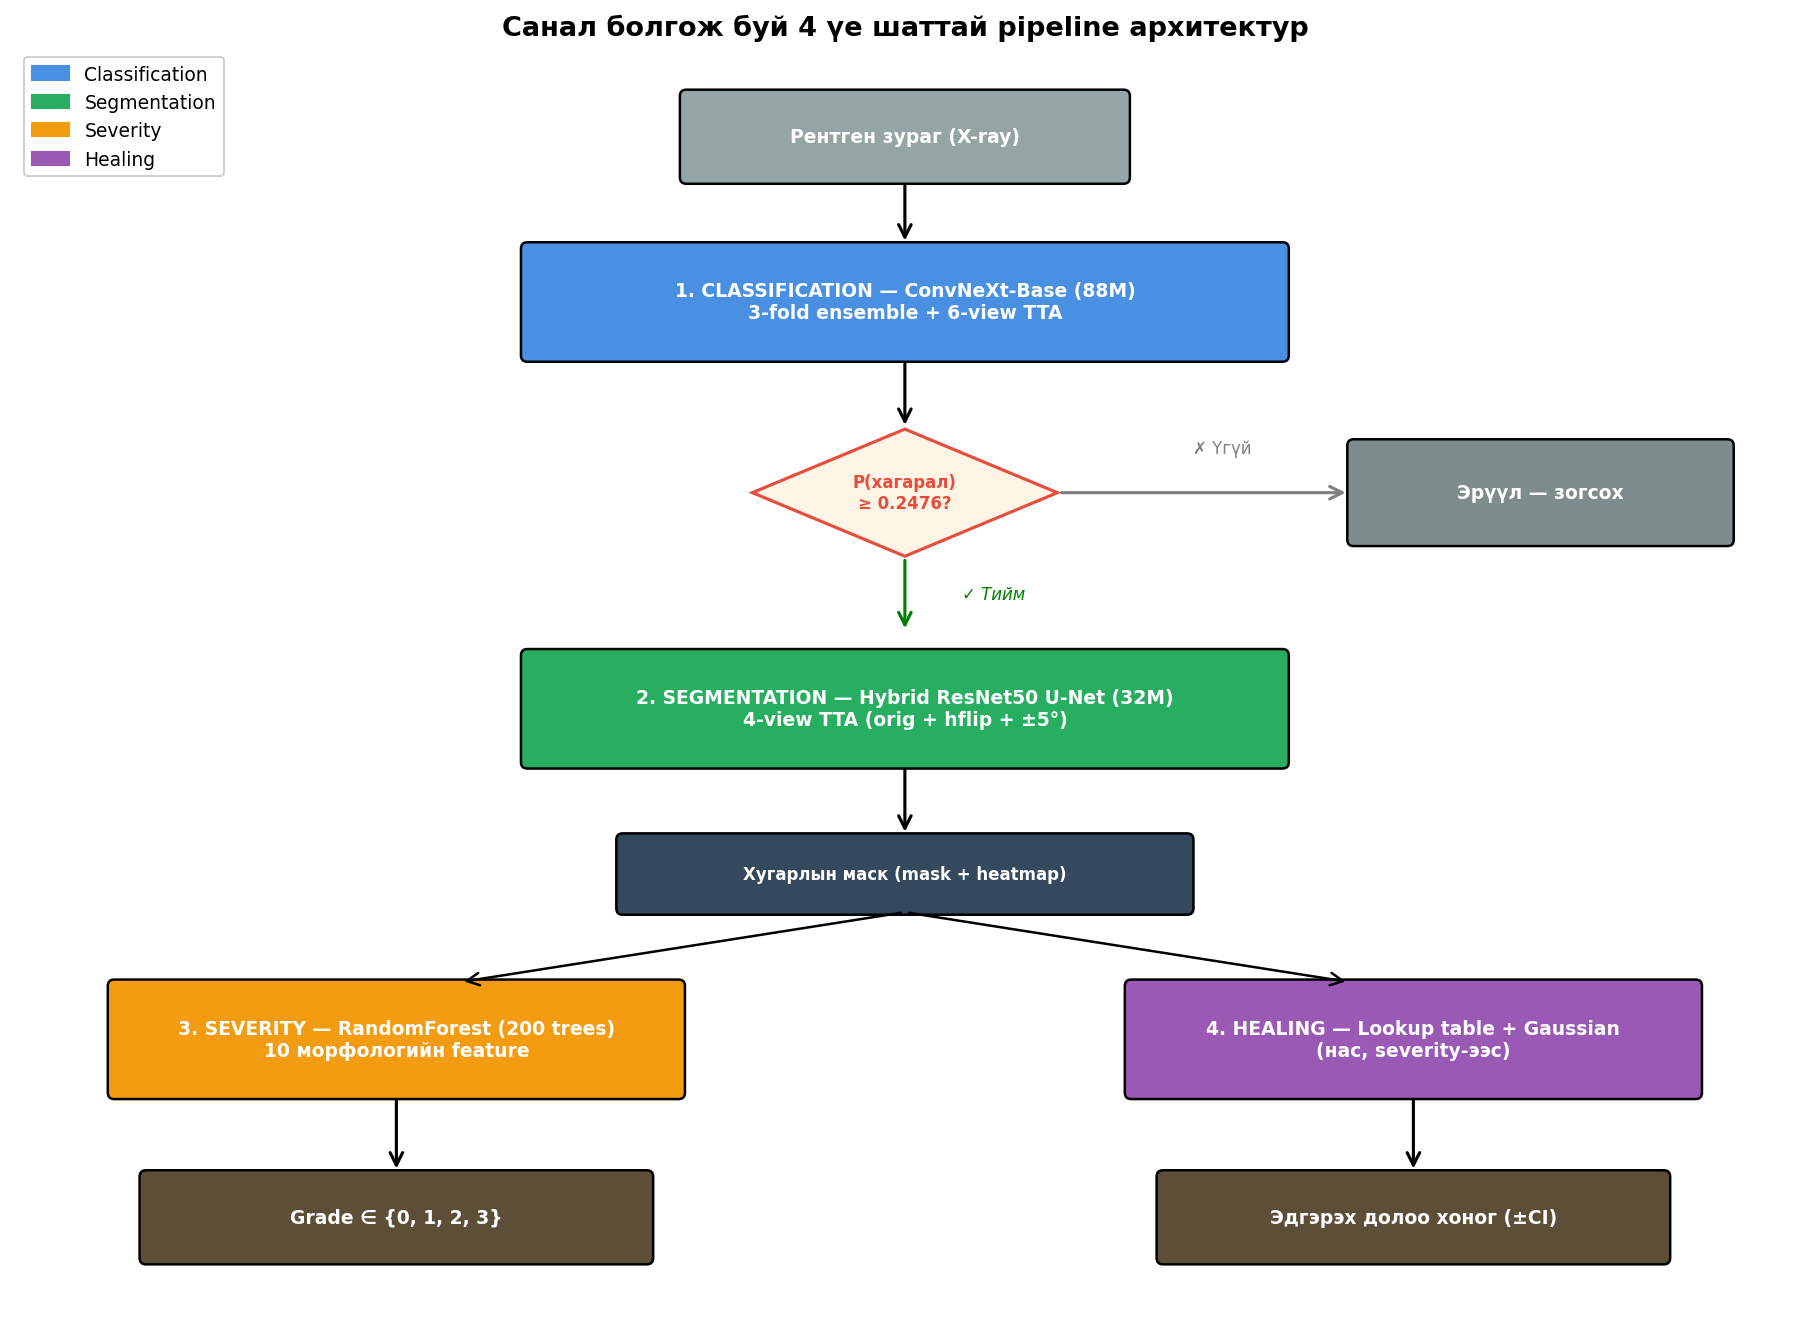
\includegraphics[width=\textwidth]{Figures/Figure_5_1.png}
\figcaption{Санал болгож буй pipeline архитектур}{Санал болгож буй дөрвөн үе шаттай модульчлагдсан pipeline архитектур}
\label{fig:proposed_arch}
\end{figure}

%───────────────────────────────────────────────────────────────────────────────
\section{Сургалтын pipeline}

Сургалтын pipeline нь өгөгдөл цуглуулах, урьдчилан боловсруулах, загвар сургах, үнэлэх болон үр дүнг тайлбарлах гэсэн үндсэн үе шатуудаас бүрдэнэ.

Эхний хоёр туршилтад MURA өгөгдлийн санг ангиллын суурь сургалтад ашигласан. Харин эцсийн буюу гурав дахь туршилтын ангиллын модульд GRAZPEDWRI-DX, FracAtlas-COCO, YOLOBoneFracture болон BoneFractureCVProject өгөгдлийн сангуудыг нэгтгэн ашиглав. FracAtlas өгөгдлийг эцсийн pipeline-д голчлон сегментчлэл болон хугарлын зэргийн үнэлгээнд хэрэглэсэн. Өгөгдлийг сургалт, баталгаажуулалт болон тестийн багцуудад хувааж, дүрсийн хэмжээг нэгэн жигд болгож, нормчлол болон өгөгдөл нэмэгдүүлэх аргуудыг хэрэгжүүлэв.

Үүний дараа ангилал болон сегментчлэлийн загваруудыг тус тус сургаж, үр дүнг баталгаажуулалтын өгөгдлөөр үнэлэв. Хугарлын зэрэг болон эдгэрэлтийн үнэлгээний модулиуд нь өмнөх үе шатуудаас гарсан үр дүнг ашиглан ажиллана.

Зураг~\ref{fig:training_pipeline}-т сургалтын ерөнхий pipeline-ийг харуулав.

\begin{figure}[!htbp]
\centering
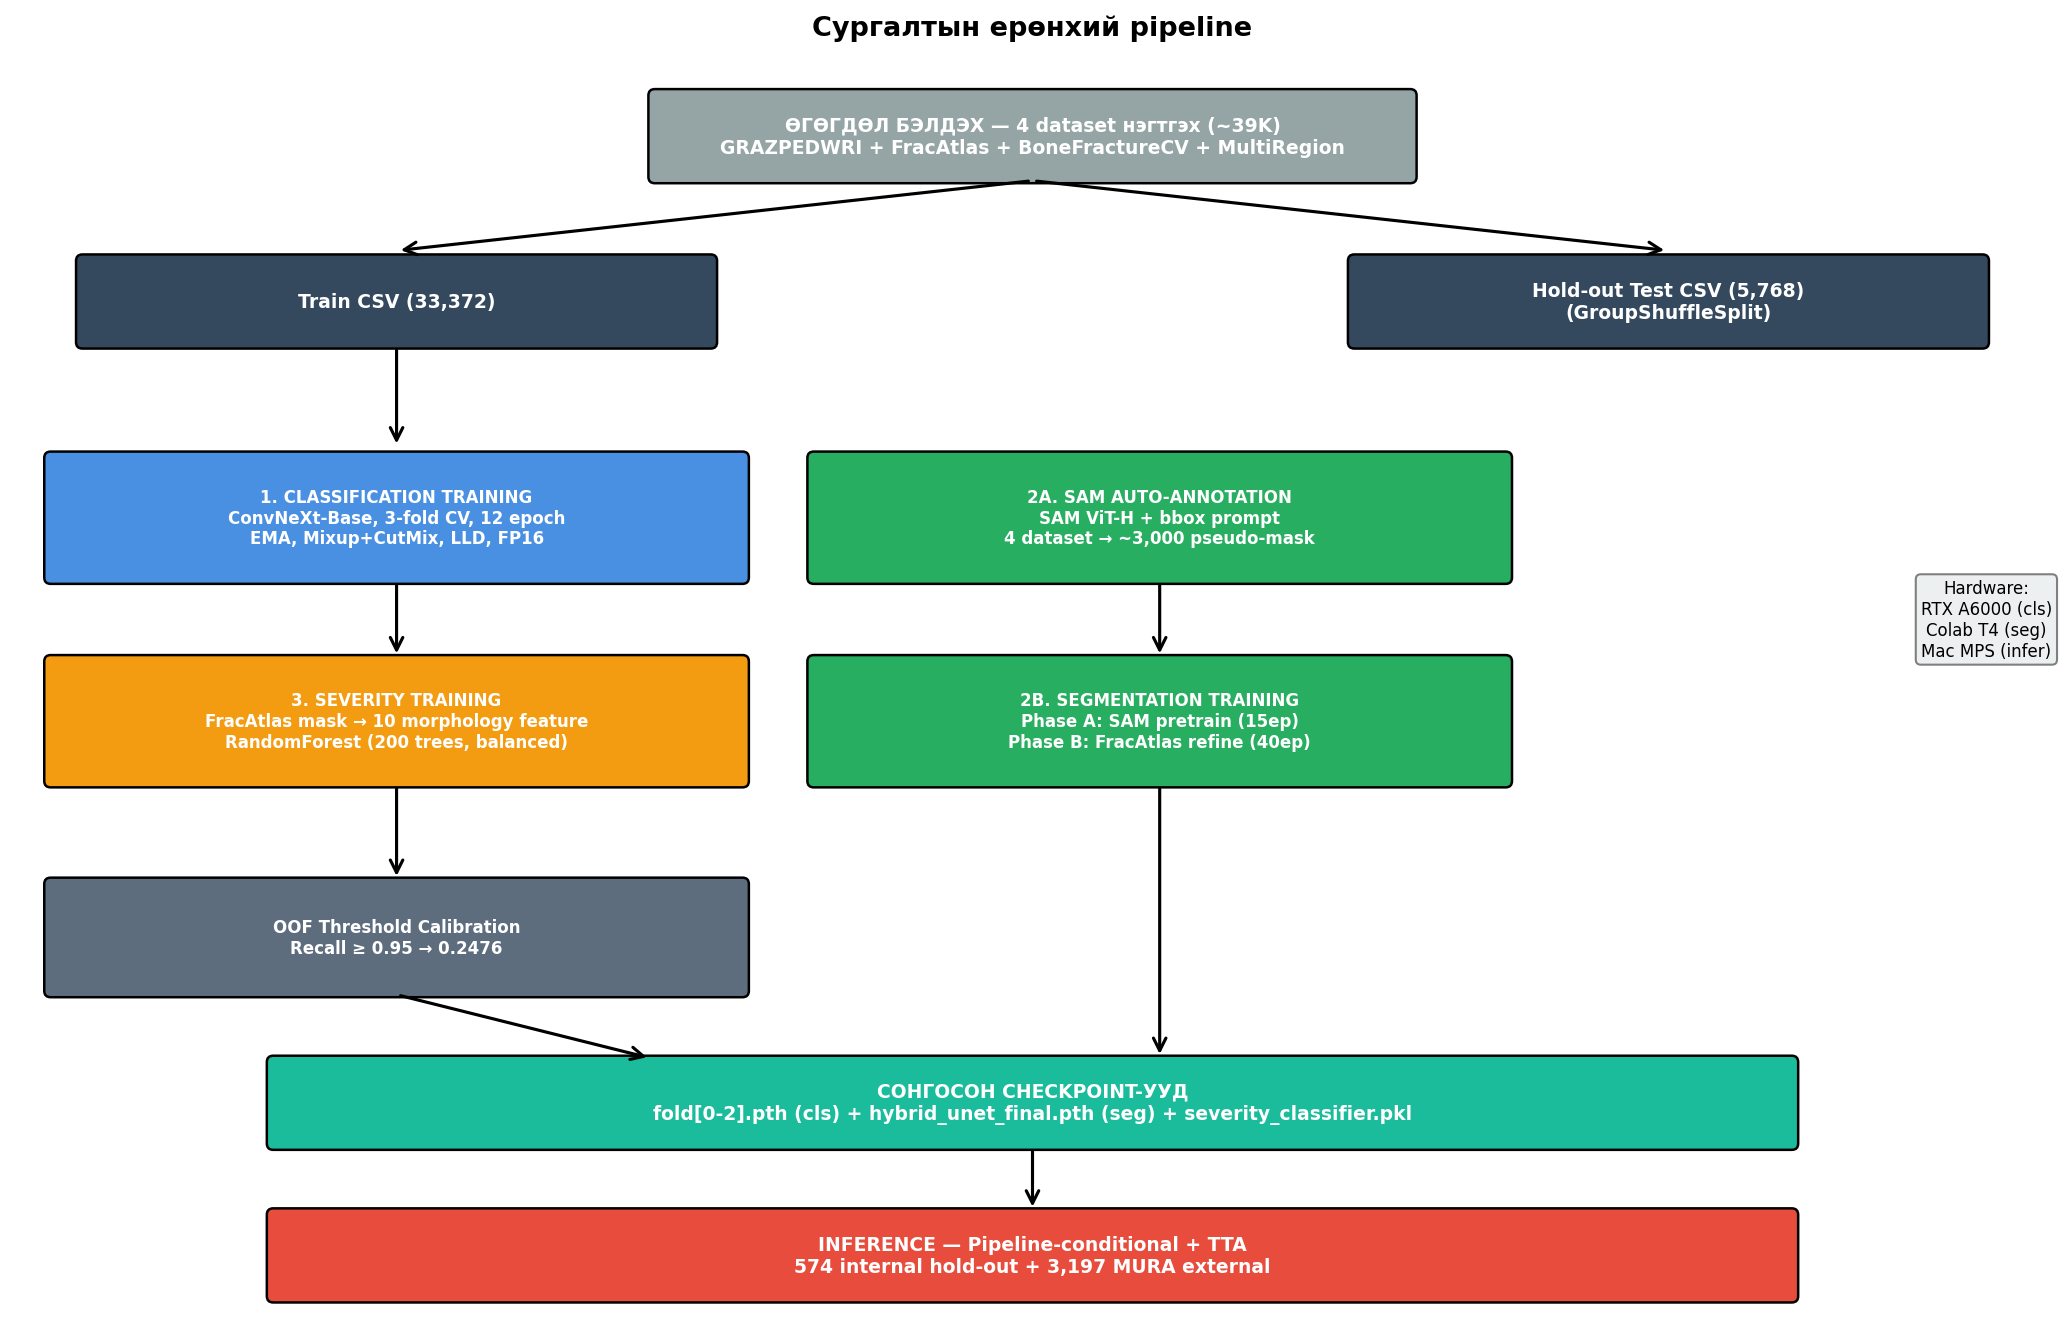
\includegraphics[width=\textwidth]{Figures/Figure_5_2.png}
\figcaption{Сургалтын ерөнхий pipeline}{Сургалтын ерөнхий pipeline — өгөгдөл цуглуулах, урьдчилан боловсруулах, загвар сургах, үнэлэх болон үр дүнг тайлбарлах үндсэн үе шатууд}
\label{fig:training_pipeline}
\end{figure}

%───────────────────────────────────────────────────────────────────────────────
\section{Туршилтын тохиргоо}

Туршилтын орчныг даалгаврын тооцооллын шаардлагаас хамааруулан хуваарилсан. Эхний хоёр туршилтын сургалтыг NVIDIA RTX A6000 (48\,GB) GPU бүхий dedicated сервер дээр гүйцэтгэсэн. Гурав дахь туршилтын ангиллын модулийг мөн RTX A6000 сервер дээр сургасан бол сегментчлэл, хугарлын зэрэг, эдгэрэлтийн модуль болон нэгдсэн inference кодыг Google Colab орчны T4 GPU дээр ажиллуулав. Загваруудыг PyTorch framework дээр (timm болон segmentation\_models\_pytorch номын сангуудтай) хэрэгжүүлж, сургалтын явцад AdamW оновчлогч ашигласан.

Сургалтын үед сегментчлэлийн модулийн дүрсийн хэмжээг $512\times512$ пиксел болгон өөрчилж, өгөгдөл нэмэгдүүлэх аргуудыг ашиглан сургалтын багцын төрөлжилтийг нэмэгдүүлэв. Давтан туршилтын үр дүнг тогтвортой байлгахын тулд тогтмол random seed (42) ашигласан.

\textbf{Тестийн арга зүй}: Загварыг сургалтын болон баталгаажуулалтын олонлогуудаас бүрэн ялгарсан \textbf{hold-out тестийн сан}-уудад үнэлэв. (1) \textit{Дотоод hold-out тест} (574 зураг) -- FracAtlas DatasetNinja-аас 61 polygon GT-тэй хагарал + 513 эрүүл зураг (random\_state=42); pipeline-conditional үнэлгээ нь зөвхөн ангилал ``хагарал'' гэж шийдсэн зурагт сегментчлэл ажиллуулна. (2) \textit{Гадаад MURA-v1.1 validation} (3{,}197 зураг) -- Stanford ML Group-ийн валидацийн санг external benchmark болгож хэрэглэв; манай сургалтад огт ороогүй. Тестийн threshold нь сургалтын OOF дээр клиник зорилгод (recall $\ge$ 0.95) тулгуурлан calibrate хийсэн 0.2476 утга бөгөөд тестийн үед \emph{дахин тааруулаагүй} тул шударга үнэлгээний нөхцөл хадгалагдсан.

Хүснэгт~\ref{tab:setup}-д туршилтын үндсэн тохиргоонуудыг харуулав.

\begin{table}[!htbp]
\centering
\small
\begin{tabular}{l l}
\toprule
\textbf{Параметр} & \textbf{Утга} \\
\midrule
Туршилт 1--2 сургалт & NVIDIA RTX A6000 (48\,GB) dedicated server \\[3pt]
Туршилт 3 ангилал & NVIDIA RTX A6000 (48\,GB) dedicated server \\[3pt]
Туршилт 3 сегментчлэл & Google Colab, NVIDIA T4 GPU \\[3pt]
Туршилт 3 хугарлын зэрэг / эдгэрэлт & Google Colab, NVIDIA T4 GPU \\[3pt]
Нэгдсэн inference код & Google Colab, NVIDIA T4 GPU \\[3pt]
Framework                & PyTorch + timm + segmentation\_models\_pytorch \\[3pt]
Оновчлогч                & AdamW \\[3pt]
Оролтын хэмжээ           & $224\times224$ (Т1/Т2), $512\times512$ (Т3 сегментаци) \\[3pt]
Batch size               & 16--192 (даалгавраас хамаарна) \\[3pt]
Scheduler                & CosineAnnealing / ReduceLROnPlateau \\[3pt]
AMP                      & \texttt{autocast} (fp16) + GradScaler \\[3pt]
Augmentation             & CLAHE, Mixup, Flip, Rotate90, GaussNoise \\[3pt]
Random seed              & 42 \\
\bottomrule
\end{tabular}
\caption{Туршилтын үндсэн тохиргоо}
\label{tab:setup}
\end{table}

%───────────────────────────────────────────────────────────────────────────────
\section{Загваруудын харьцуулалт ба шинжилгээ}

Судалгааны явцад гурван өөр хандлага туршиж үзсэн бөгөөд тэдгээрийн үр дүнг харьцуулан шинжилсэн.

\subsection{Туршилт 1: Нэгдсэн олон даалгаварт архитектур}

Эхний туршилтад бүх даалгаврыг нэг хуваалцсан кодлогчтой архитектурт нэгтгэн сургахыг зорьсон. Энэхүү арга нь параметрийн үр ашгийг нэмэгдүүлэх давуу талтай байсан боловч даалгавруудын хоорондын зөрчил (task interference) үүсч, сегментчлэлийн чанар системтэйгээр буурсан. Тест олонлог дээр ангиллын AUC = 0.8173 хүрсэн ч сегментчлэлийн Mean Dice = 0.0498, Mean IoU = 0.0303 буюу median Dice = 0 (тест зургуудын талаас илүүд маск огт гараагүй) гарсан нь даалгавруудын зөрчлийн шууд нотолгоо болсон.

\subsection{Туршилт 2: Дараалсан сургалтын арга}

Хоёр дахь туршилтад даалгавруудыг дараалан тусдаа загварт сургах аргыг ашигласан. Энэ нь эхний туршилтаас илүү тогтвортой үр дүн үзүүлсэн: ангиллын AUC = 0.8668, баталгаажуулалтын олонлог дээр сегментчлэлийн Dice = 0.9633, хугарлын зэргийн Exact Accuracy = 0.872 хүрсэн. Гэвч баталгаажуулалтын өндөр Dice нь overfitting шинжтэй байсан тул тест дэх бодит сегментчлэлийн чанар хангалтгүй хэвээр байв.

\subsection{Туршилт 3: Сайжруулсан модульчлагдсан pipeline}

Гурав дахь туршилтад ангилал, сегментчлэл, хугарлын зэрэг үнэлэх болон эдгэрэлтийн таамаглалыг тусдаа модулиудаар хэрэгжүүлсэн. Ангилалд ConvNeXt-Base (ImageNet-22K), сегментчлэлд эрлийз ResNet50 U-Net, хугарлын зэрэгт морфологийн эвристик ашигласан. Энэхүү хандлага нь өмнөх хоёр туршилтаас илүү өндөр гүйцэтгэл үзүүлж, тест олонлог дээр ангиллын AUC = 0.9887, сегментчлэлийн Dice = 0.604, IoU = 0.433 хүрч, бүх даалгаварт хамгийн тогтвортой үр дүнд хүрсэн.

\subsection{Туршилтуудын харьцуулалт}

Хүснэгт~\ref{tab:exp_compare}-д гурван туршилтын үндсэн үзүүлэлтүүдийг харьцуулан үзүүлэв.

\begin{table}[!htbp]
\centering
\small
\begin{tabular}{l l c c c}
\toprule
\textbf{Даалгавар} & \textbf{Метрик}
  & \textbf{Т1 (нэгдсэн, test)}
  & \textbf{Т2 (тусдаа, val)}
  & \textbf{Т3 (модульч., test)} \\
\midrule
\multirow{2}{*}{Ангилал}
  & AUC-ROC & 0.8173 & 0.8668 & \textbf{0.9887} \\
  & Recall  & 0.727  & 0.685  & \textbf{0.950} \\[4pt]
\multirow{2}{*}{Сегментаци}
  & Dice & 0.0498 & 0.9633\textsuperscript{*} & \textbf{0.604} \\
  & IoU  & 0.0303 & 0.9441\textsuperscript{*} & \textbf{0.433} \\[4pt]
\multirow{2}{*}{Хугарлын зэрэг}
  & Exact Acc & 0.556 & 0.872 & \textbf{1.000}\textsuperscript{†} \\
  & MAE       & 0.535 & 0.213 & \textbf{---} \\[4pt]
Эдгэрэлт & $R^2$ & --- & 0.459 & 0.459 \\
\bottomrule
\multicolumn{5}{l}{\footnotesize\textsuperscript{*}Validation overfitting шинжтэй --- тест дэх бодит Dice $=0.604$} \\
\multicolumn{5}{l}{\footnotesize\textsuperscript{†}Тест олонлогт зөвхөн Class~1--2 байсан (Class~0, 3 байгаагүй)}
\end{tabular}
\caption{Гурван туршилтын харьцуулалт}
\label{tab:exp_compare}
\end{table}

Харьцуулалтын үр дүнгээс харахад модульчлагдсан pipeline нь олон даалгаварт архитектуртай харьцуулахад илүү тогтвортой бөгөөд сегментчлэл болон хугарлын зэрэг үнэлэх даалгаварт өндөр гүйцэтгэл үзүүлсэн. Тухайлбал сегментчлэлийн Dice нэгдсэн загварт 0.0498 байсан бол модульчлагдсан pipeline-д 0.604 болж $\approx$12 дахин нэмэгдсэн нь task interference-ийг арилгасны шууд үр дүн юм. Гурван туршилтын тоон үр дүнг илүү нарийвчлан Бүлэг~\ref{Chapter6}-д авч үзнэ.

%───────────────────────────────────────────────────────────────────────────────
\section{Бүрэлдэхүүн хэсгийн нөлөөллийн шинжилгээ}

Санал болгож буй pipeline-ийн бүрэлдэхүүн хэсгүүдийн нөлөөг үнэлэх зорилгоор бүрэлдэхүүн хэсгийн нөлөөллийн шинжилгээ (ablation study) хийв. Эхний хувилбарт зөвхөн ангиллын модуль ашигласан бол дараагийн хувилбаруудад сегментчлэл, хугарлын зэрэг үнэлгээ болон эдгэрэлтийн таамаглалын модулиудыг үе шаттайгаар нэмсэн.

Үр дүнгээс харахад сегментчлэлийн модуль нэмэгдсэнээр хугарлын байршлыг илүү нарийвчлалтай тодорхойлох боломж бүрдсэн. Харин хугарлын зэрэг болон эдгэрэлтийн модулиуд нь клиникийн эцсийн шийдвэр гаргах түвшний баталгаажсан загвар бус, pipeline-ийн дараагийн шатанд ямар төрлийн мэдээлэл гаргаж болохыг шалгасан proof-of-concept бүрэлдэхүүнүүд болно. Иймээс эдгээр модулийн үр дүнг эмчийн үнэлгээтэй шууд дүйцүүлэхгүй, цаашид бодит клиникийн шошго болон follow-up өгөгдлөөр баталгаажуулах шаардлагатай.

Хүснэгт~\ref{tab:ablation_modules}-т нөлөөллийн шинжилгээний үр дүнг үзүүлэв.

\begin{table}[!htbp]
\centering
\small
\begin{tabular}{l l l c c}
\toprule
\textbf{Хувилбар} & \textbf{Идэвхтэй модулиуд} & \textbf{Гол метрик} & \textbf{Үр дүн} & \textbf{Нэмэгдсэн чадвар} \\
\midrule
A1 & Ангилал                          & AUC-ROC   & 0.9887 & Хугарал илрүүлэх \\[3pt]
A2 & \quad + Сегментаци               & Dice      & 0.604  & Хугарлын байршил \\[3pt]
A3 & \quad + Хугарлын зэрэг           & Exact Acc & 1.000\textsuperscript{†}  & Клиник зэрэглэл \\[3pt]
A4 & \quad + Эдгэрэлт (бүрэн pipeline) & $R^2$     & 0.459  & Эдгэрэлтийн хугацаа \\
\bottomrule
\multicolumn{5}{l}{\footnotesize Метрик бүр тухайн модулийн тест/баталгаажуулалтын олонлог дээрх бодит утга.} \\
\multicolumn{5}{l}{\footnotesize\textsuperscript{†}Тест олонлогт зөвхөн Class~1--2 байсан.}
\end{tabular}
\caption{Pipeline модулиудын нөлөөллийн шинжилгээ}
\label{tab:ablation_modules}
\end{table}

Нөлөөллийн шинжилгээнээс харахад модуль бүр pipeline-д тусдаа функциональ үнэ цэнэ нэмж байгаа нь харагдана: ангилал хугарлыг илрүүлж, сегментаци байршлыг тогтоож, морфологийн эвристик хугарлын зэргийн proof-of-concept үнэлгээ гаргаж, эдгэрэлтийн модуль цаашдын төлөвийн proof-of-concept таамаглал үүсгэснээр дөрвөн үе шаттай судалгааны pipeline бүрдэв. Ангилал болон сегментчлэлийн модулиудын сургалтын аргын дотоод нөлөөллийн шинжилгээ (ablation: Focal BCE, CLAHE, Mixup, хоёр үе шаттай сургалт, TTA)-ийг Бүлэг~\ref{Chapter6}-д нарийвчлан авч үзнэ.


%\include{Chapters/bib} 

%-------------------------------------------------------------------------------
%	THESIS CONTENT - APPENDICES
%-------------------------------------------------------------------------------

\appendix % Дараах "chapter" нь Хавсралт болохыг LaTeX-д хэлэх
% Нэг л "Хавсралт" бүлэг (дотроо section-уудтай). Зураг/хүснэгтийг Х.N хэлбэрээр дугаарлана.
\renewcommand{\thechapter}{}
\renewcommand{\thesection}{\arabic{section}}
\renewcommand{\thefigure}{Х.\arabic{figure}}
\renewcommand{\thetable}{Х.\arabic{table}}
\pagecolor{white}
% !TEX root = ../main.tex
% Нэгдсэн хавсралт

\chapter{Хавсралт}
\label{Appendix}
\pagecolor{white}

%───────────────────────────────────────────────────────────────────────────────
\section{Судалгаанд ашигласан өгөгдлийн сангууд}

Энэхүү судалгаанд ясны хугарлын ангилал, сегментчлэл болон үнэлгээний даалгавруудад зориулан олон нийтэд нээлттэй хэд хэдэн өгөгдлийн санг ашиглав. MURA өгөгдлийг эхний хоёр туршилтын ангиллын суурь сургалтад ашигласан бол эцсийн модульчлагдсан pipeline-д бусад эх сурвалжуудыг ашигласан. Хүснэгт~\ref{tab:appA_datasets}-д ашигласан өгөгдлийн сангуудын үндсэн мэдээллийг харуулав.

\begin{table}[ht]
    \centering
    \begin{tabular}{|l|c|l|}
    \hline
    \textbf{Өгөгдлийн сан} & \textbf{Зургийн тоо} & \textbf{Даалгавар} \\ \hline
    MURA                  & $\sim$40{,}000 & Туршилт 1--2, ангиллын суурь сургалт \\ \hline
    FracAtlas             & 4{,}083  & Сегментчлэл, хугарлын зэрэг \\ \hline
    FracAtlas-COCO        & 966      & Туршилт 3-ын ангилал \\ \hline
    GRAZPEDWRI-DX         & 20{,}327 & Туршилт 3-ын ангилал \\ \hline
    YOLOBoneFracture      & 3{,}979  & Туршилт 3-ын ангилал, псевдо маск \\ \hline
    BoneFractureCVProject & 3{,}631  & Туршилт 3-ын ангилал, псевдо маск \\ \hline
    \end{tabular}
    \caption{Судалгаанд ашигласан өгөгдлийн сангууд}
    \label{tab:appA_datasets}
\end{table}

Эцсийн модульчлагдсан pipeline-д MURA-г оруулахгүйгээр нийтдээ 30{,}000 гаруй (нийлбэр $\approx$32{,}986) рентген зургийг боловсруулж ашигласан. Харин эхний хоёр туршилтын ангиллын суурь сургалтад MURA-ийн $\sim$40{,}000 зургийг тусад нь ашигласан болно.

%───────────────────────────────────────────────────────────────────────────────
\section{Хугарлын зэрэг үнэлгээний геометрийн шинж}

Хугарлын сегментчлэлийн үр дүнд үндэслэн морфологийн шинжүүдийг гарган авч хугарлын зэргийг үнэлсэн. Хүснэгт~\ref{tab:appE_geom}-д нэг жишээ тохиолдол (Grade~2)-д тооцоолсон геометрийн шинжүүдийг үзүүлэв. Хугарлын зэргийн дүрслэлийн жишээнүүдийг үндсэн үр дүнгийн бүлэгт (Бүлэг~\ref{Chapter6}) харуулсан болно.

\begin{table}[ht]
    \centering
    \begin{tabular}{|l|c|}
    \hline
    \textbf{Үзүүлэлт} & \textbf{Утга} \\ \hline
    Area (талбай, px$^2$)         & 1{,}872 \\ \hline
    Major axis (гол тэнхлэг, px)  & 55.41 \\ \hline
    Aspect Ratio (тал харьцаа)    & 1.23 \\ \hline
    Solidity (нягтрал)            & 1.00 \\ \hline
    Severity Score (зэргийн оноо) & 2 (Grade~2) \\ \hline
    \end{tabular}
    \caption{Геометрийн шинжүүдийн жишээ (Grade~2 тохиолдол)}
    \label{tab:appE_geom}
\end{table}

%───────────────────────────────────────────────────────────────────────────────
\section{Туршилтын орчин ба тохиргоо}

Туршилтуудыг гүйцэтгэхэд ашигласан техник болон програм хангамжийн орчин, сургалтын үндсэн тохиргоог дараах хүснэгтүүдэд нэгтгэн үзүүлэв.

\begin{table}[ht]
    \centering
    \begin{tabular}{|l|l|}
    \hline
    \textbf{Модуль / туршилт} & \textbf{Орчин} \\ \hline
    Туршилт 1--2 сургалт & NVIDIA RTX A6000 (48 GB) dedicated server \\ \hline
    Туршилт 3 ангилал & NVIDIA RTX A6000 (48 GB) dedicated server \\ \hline
    Туршилт 3 сегментчлэл & Google Colab, NVIDIA T4 GPU \\ \hline
    Туршилт 3 хугарлын зэрэг, эдгэрэлт & Google Colab, NVIDIA T4 GPU \\ \hline
    Нэгдсэн inference код & Google Colab, NVIDIA T4 GPU \\ \hline
    \end{tabular}
    \caption{Туршилтад ашигласан техник хангамжийн орчин}
    \label{tab:appH_hw}
\end{table}

\begin{table}[ht]
    \centering
    \begin{tabular}{|l|l|l|}
    \hline
    \textbf{Програм / сан} & \textbf{Хувилбар} & \textbf{Зориулалт} \\ \hline
    Python                       & 3.10            & Үндсэн програмчлалын хэл \\ \hline
    PyTorch (torch)              & 2.1 (cu121)     & Гүн сургалтын фреймворк \\ \hline
    torchvision                  & 0.16            & Дүрсний хувиргалт, загвар \\ \hline
    CUDA                         & 12.1            & GPU тооцоолол \\ \hline
    timm                         & 1.0             & ConvNeXt, EfficientNet backbone \\ \hline
    segmentation-models-pytorch  & 0.3             & ResNet50 U-Net сегментчлэл \\ \hline
    Segment Anything (SAM)       & ViT-B           & Псевдо маск үүсгэх \\ \hline
    albumentations               & 1.4             & Өгөгдөл нэмэгдүүлэлт \\ \hline
    OpenCV (opencv-python)       & 4.9             & Дүрс боловсруулалт \\ \hline
    NumPy                        & 1.26            & Тоон тооцоолол \\ \hline
    Pandas                       & 2.2             & Өгөгдөл боловсруулалт \\ \hline
    scikit-learn                 & 1.4             & Random Forest (хугарлын зэрэг) \\ \hline
    scikit-image                 & 0.22            & Морфологийн шинж тооцоолол \\ \hline
    SciPy                        & 1.11            & Шинжлэх ухааны тооцоолол \\ \hline
    pytorch-grad-cam             & 1.5             & Grad-CAM тайлбарлалт \\ \hline
    SHAP                         & 0.44            & SHAP тайлбарлалт \\ \hline
    Matplotlib                   & 3.8             & График дүрслэл \\ \hline
    \end{tabular}
    \caption{Програм хангамж}
    \label{tab:appH_sw}
\end{table}

\begin{table}[ht]
    \centering
    \begin{tabular}{|l|l|}
    \hline
    \textbf{Үзүүлэлт} & \textbf{Утга} \\ \hline
    Batch Size    & 16 \\ \hline
    Epochs        & 50 (10 хөлдөөсөн + 40 бүрэн) \\ \hline
    Optimizer     & AdamW \\ \hline
    Learning Rate & $1\times10^{-4}$ \\ \hline
    Image Size    & $512\times512$ \\ \hline
    Random Seed   & 42 \\ \hline
    \end{tabular}
    \caption{Сургалтын үндсэн тохиргоо}
    \label{tab:appH_train}
\end{table}

%───────────────────────────────────────────────────────────────────────────────
\section{Судалгааны кодын GitHub репозитор}

Судалгааны ажлын эх код, туршилтын сургалт болон inference хийхэд ашигласан script, notebook, мөн дипломын тайлангийн \LaTeX{} эх файлуудыг GitHub репозиторт байршуулсан. Репозиторийн холбоос: \href{https://github.com/Ariuntungalag23/diploma}{\texttt{github.com/Ariuntungalag23/diploma}}.

Репозиторт ангилал, сегментчлэл, хугарлын зэрэг болон эдгэрэлтийн төлөвийг үнэлэх proof-of-concept модулиудын код, туршилтын туслах script-үүд, тайлангийн эх материалууд багтсан. Харин өгөгдлийн сан, сургасан model weight, checkpoint, завсрын үр дүнгийн том хэмжээтэй файл болон хувийн тохиргооны файлуудыг хэмжээ, лиценз, нууцлалын шалтгаанаар оруулаагүй. Эдгээр файлыг репозиторийн \texttt{.gitignore} тохиргоогоор тусгаарласан бөгөөд өгөгдлийг тухайн олон нийтэд нээлттэй эх сурвалжаас тусад нь татаж ашиглах шаардлагатай.

Эцсийн хувилбарыг GitHub-д \texttt{diploma\_ariuntungalag} commit нэрээр байршуулсан. Энэ нь судалгаанд ашигласан кодын бүтцийг шалгах, туршилтын pipeline-ийг давтан ажиллуулах болон тайлангийн эхийг хянах боломжийг бүрдүүлнэ.

%───────────────────────────────────────────────────────────────────────────────
\section{Хиймэл оюуны хэрэгслийн ашиглалт}

Энэхүү судалгааны ажлын явцад хиймэл оюуны хэрэгслүүдийг зөвхөн туслах зориулалтаар ашигласан.

\begin{table}[ht]
    \centering
    \begin{tabular}{|l|l|}
    \hline
    \textbf{Хэрэгсэл} & \textbf{Ашигласан зориулалт} \\ \hline
    ChatGPT        & Бичвэрийн найруулга, хэл зүй болон үг үсгийн алдаа шалгах \\ \hline
    GitHub Copilot & Кодын автомат гүйцээлт, алдаа засахад туслах \\ \hline
    \end{tabular}
    \caption{AI хэрэгслийн ашиглалт}
    \label{tab:appI_ai}
\end{table}

Хиймэл оюуны хэрэгслүүдийг судалгааны үр дүн, туршилтын хэмжилт, статистик тооцоолол болон эцсийн дүгнэлтийг автоматаар үүсгэхэд ашиглаагүй болно. Судалгааны бүх туршилт, өгөгдөл боловсруулалт, үр дүнгийн үнэлгээ болон шинжилгээг судлаач өөрөө гүйцэтгэсэн болно.

%───────────────────────────────────────────────────────────────────────────────
\section{Нэмэлт зураг}

Энэ хэсэгт үндсэн бүлгийн хэлэлцүүлгийг нэмж тодотгох зорилгоор сегментчлэлийн нэмэлт жишээ, нэгдсэн pipeline-ийн жишээ дүгнэлт болон модуль хоорондын зөрчлийн нэмэлт жишээг үзүүлэв.

\begin{figure}[H]
    \centering
    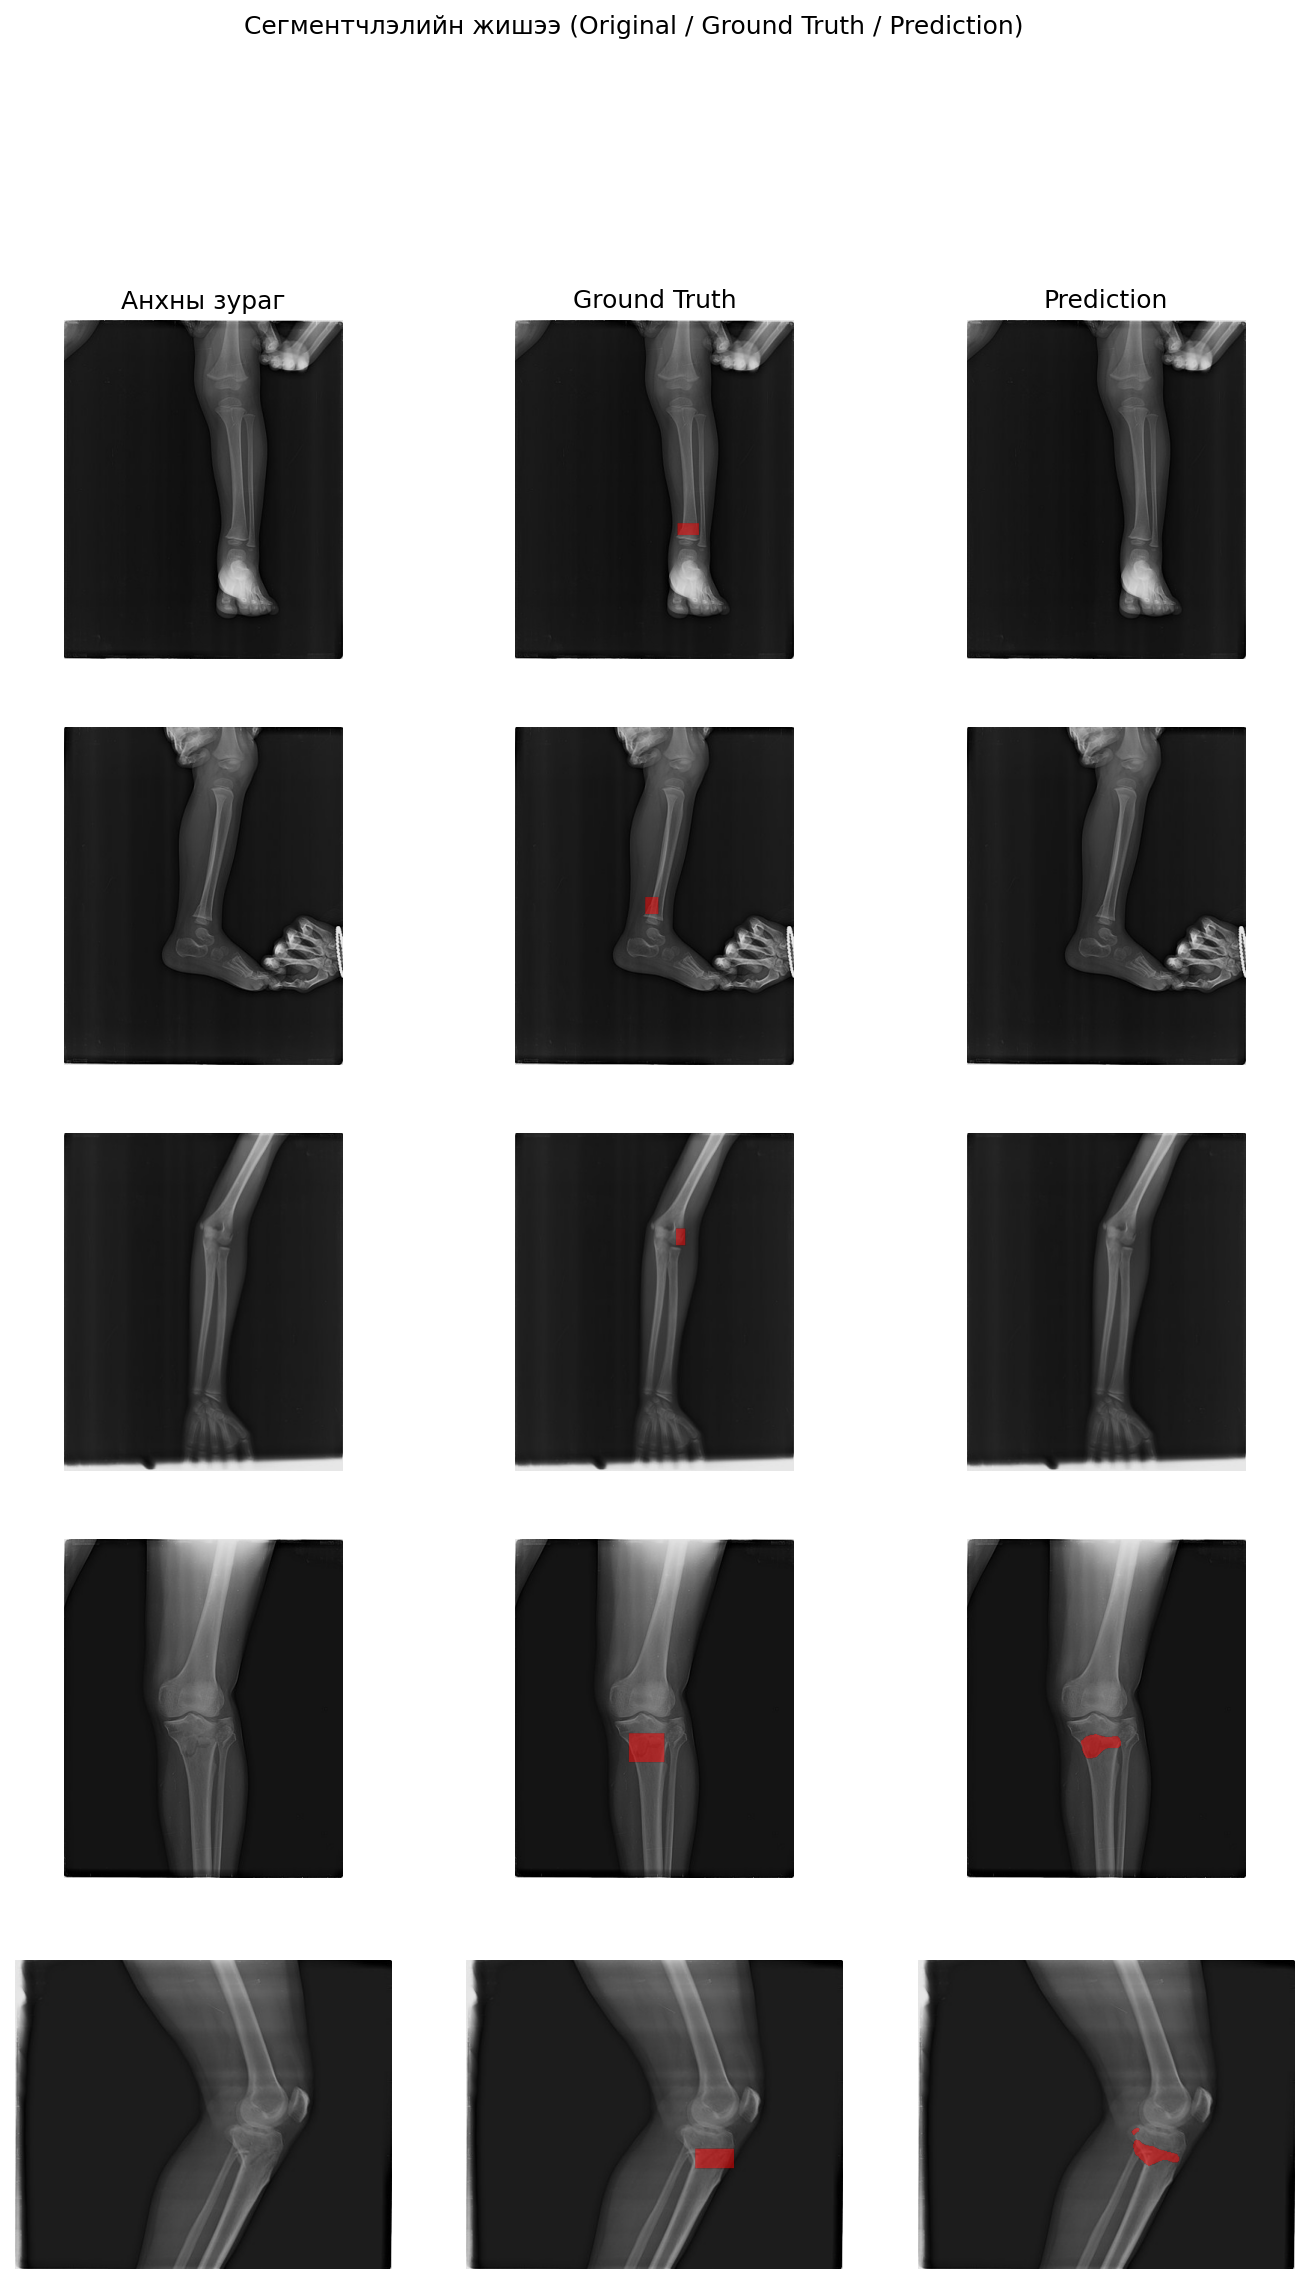
\includegraphics[width=\textwidth,height=0.85\textheight,keepaspectratio]{Figures/appx_d3_seg_triplets.png}
    \figcaption{Нэмэлт сегментчлэлийн жишээнүүд}{Нэмэлт сегментчлэлийн жишээнүүд — анхны рентген зураг, лавлах маск (GT) болон загварын таамагласан маскийн харьцуулалт}
    \label{fig:seg_more}
\end{figure}

\begin{figure}[H]
    \centering
    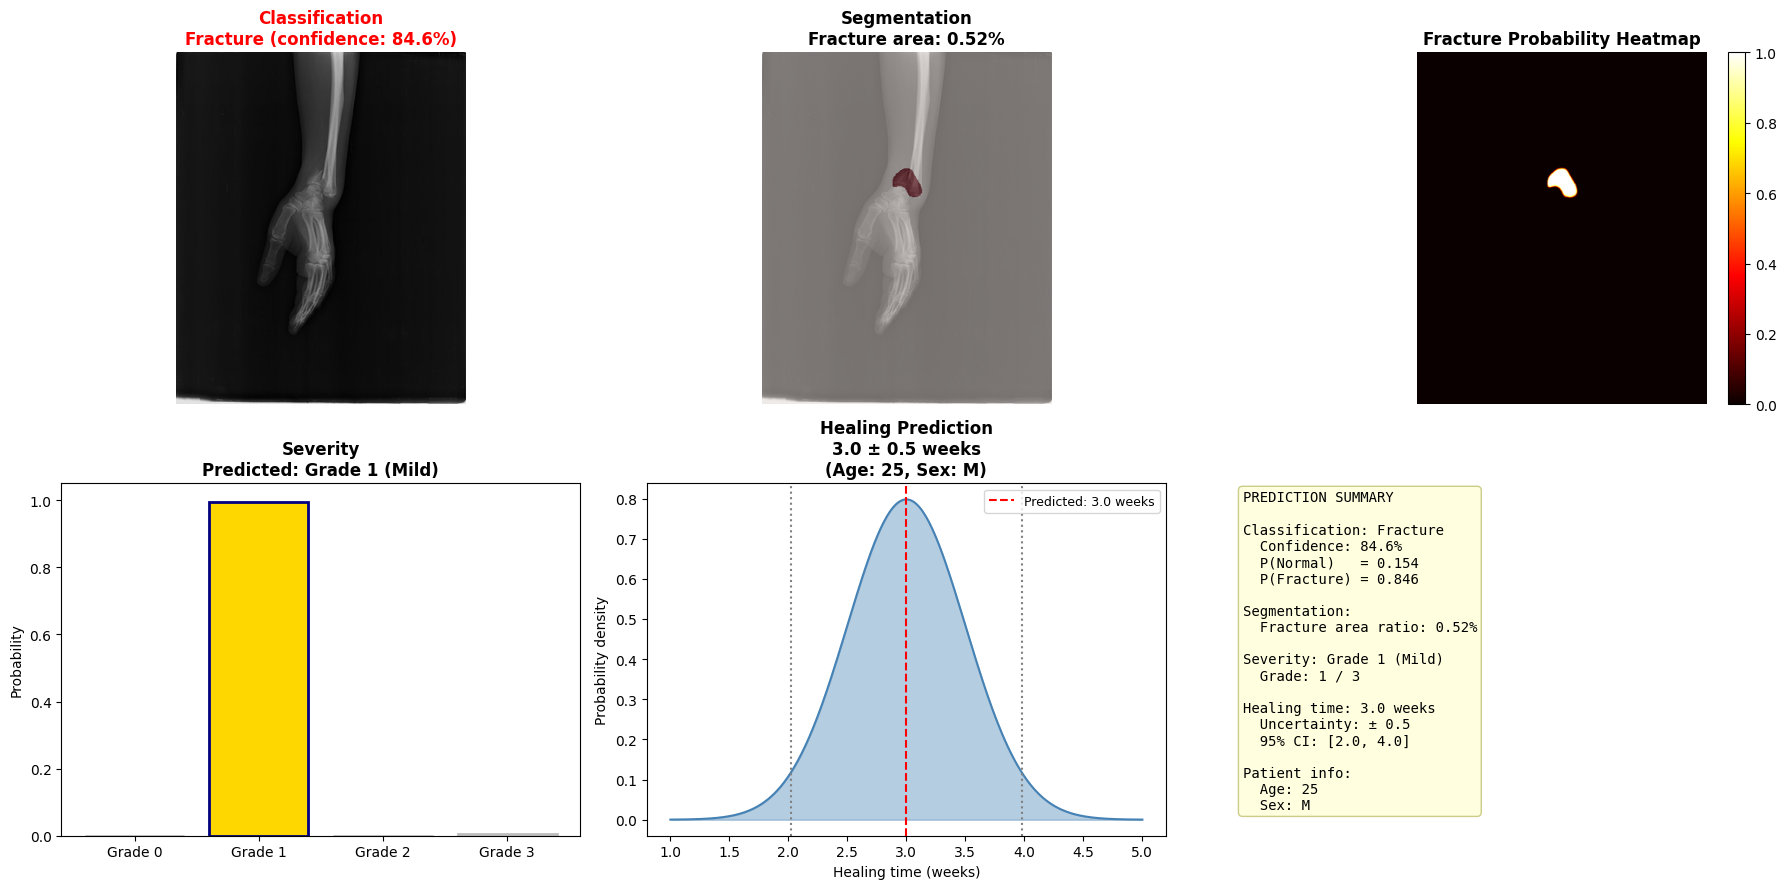
\includegraphics[width=\textwidth]{Figures/t3_predict_example.png}
    \figcaption{Бугуйн хугарлын жишээ таамаглал}{Бугуйн хугарлын жишээ таамаглал: ангилал \emph{Fracture} (итгэл 84.6\%), Grade~1 (Mild), эдгэрэлт $\approx$3 долоо хоног}
    \label{fig:pred_wrist}
\end{figure}

\begin{figure}[H]
    \centering
    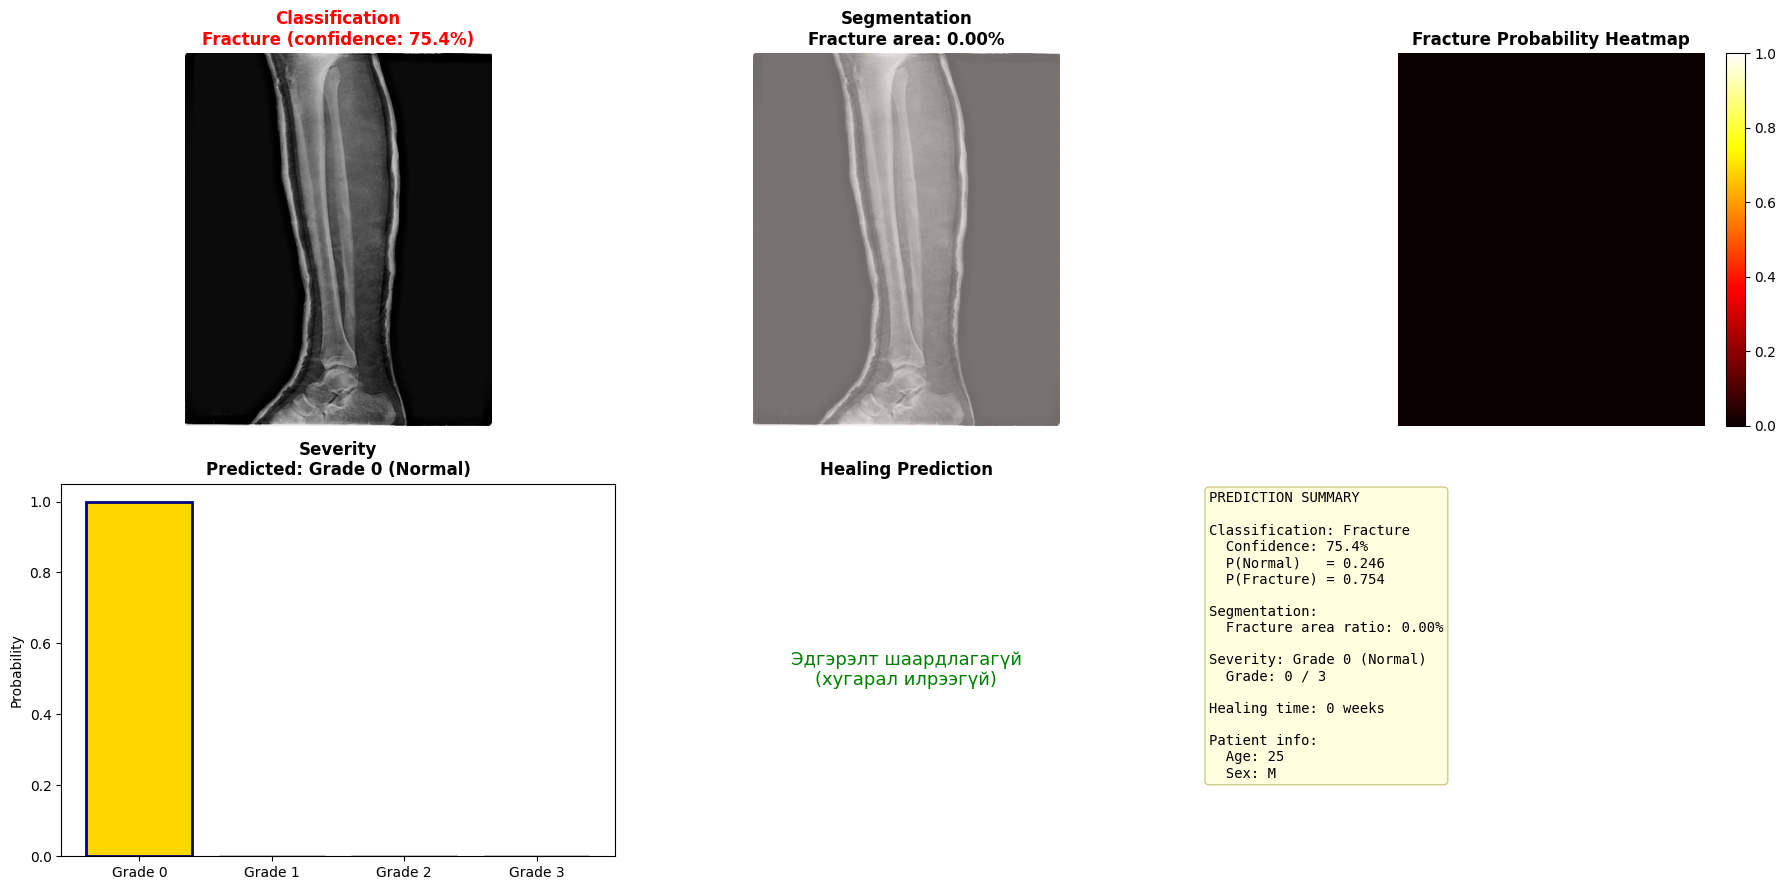
\includegraphics[width=\textwidth]{Figures/t3_pred_demo_9.png}
    \figcaption{Модуль хоорондын зөрчлийн жишээ 2}{Модуль хоорондын зөрчлийн өөр жишээ (IMG0003704): $P=0.754$ боловч маск гараагүй}
    \label{fig:err_disagree2}
\end{figure}


%-------------------------------------------------------------------------------
%	BIBLIOGRAPHY
%-------------------------------------------------------------------------------
\defformat % Бүлгийн нэрийг оргиналь байдлаар хэвлэх
\patchcmd{\chapter}{\pagecolor{Beige}}{\pagecolor{white}}{}{}
\pagecolor{white}
\addchaptertocentry{Ашигласан материалын жагсаалт} % Ашигласан материалыг гарчигт нэмэх

\printbibliography[heading=bibliography,title={Ашигласан материалын жагсаалт}]

%-------------------------------------------------------------------------------

\end{document}
